%%%%%%%%%%%%%%%%%%%%%%%%%%%%%%%%%%%%%%%%%%  不使用 authblk 包制作标题  %%%%%%%%%%%%%%%%%%%%%%%%%%%%%%%%%%%%%%%%%%%%%%
%-------------------------------PPT Title-------------------------------------
\title{第一原理计算理论与方法导论}
%-----------------------------------------------------------------------------

%----------------------------Author & Date------------------------------------
%\author[\textrm{Jun\_Jiang}]{姜\;\;骏\inst{}} %[]{} (optional, use only with lots of authors)
%% - Give the names in the same order as the appear in the paper.
%% - Use the \inst{?} command only if the authors have different
%%   affiliation.
\institute[BCC]{\inst{}%
%\institute[Gain~Strong]{\inst{}%
\vskip -20pt 北京市计算中心~云平台事业部}
%\vskip -20pt {\large 格致斯创~科技}}
\date[\today] % (optional, should be abbreviation of conference name)
{%	{\fontsize{6.2pt}{4.2pt}\selectfont{\textcolor{blue}{E-mail:~}\url{jiangjun@bcc.ac.cn}}}
\vskip 45 pt {\fontsize{8.2pt}{6.2pt}\selectfont{%清华大学\;\;物理系% 报告地点
	\vskip 5 pt \textrm{2023.05}}}
}

%% - Either use conference name or its abbreviation
%% - Not really information to the audience, more for people (including
%%   yourself) who are reading the slides onlin%%   yourself) who are reading the slides onlin%%   yourself) who are reading the slides onlineee
%%%%%%%%%%%%%%%%%%%%%%%%%%%%%%%%%%%%%%%%%%%%%%%%%%%%%%%%%%%%%%%%%%%%%%%%%%%%%%%%%%%%%%%%%%%%%%%%%%%%%%%%%%%%%%%%%%%%%

\subject{}
% This is only inserted into the PDF information catalog. Can be left
% out.
%\maketitle
\frame
{
%	\frametitle{\fontsize{9.5pt}{5.2pt}\selectfont{\textcolor{orange}{“高通量并发式材料计算算法与软件”年度检查}}}
\titlepage
}
%-----------------------------------------------------------------------------

%------------------------------------------------------------------------------列出全文 outline ---------------------------------------------------------------------------------
\section*{}
\frame[allowframebreaks]
{
  \frametitle{Outline}
%  \frametitle{\textcolor{mycolor}{\secname}}
  \tableofcontents%[current,currentsection,currentsubsection]
}
%%在每个section之前列出全部Outline
%%类似的在每个subsection之前列出全部Outline是\AtBeginSubsection[]
%\AtBeginSection[]
%{
%  \frame<handout:0>%[allowframebreaks]
%  {
%    \frametitle{Outline}
%%全部Outline中,本部分加亮
%    \tableofcontents[current,currentsection]
%  }
%}

%-----------------------------------------------PPT main Body------------------------------------------------------------------------------------
\small
\section{引言}
\frame
{
	\frametitle{材料模拟的作用与地位}
\begin{figure}[h!]
\vspace*{-0.18in}
\centering
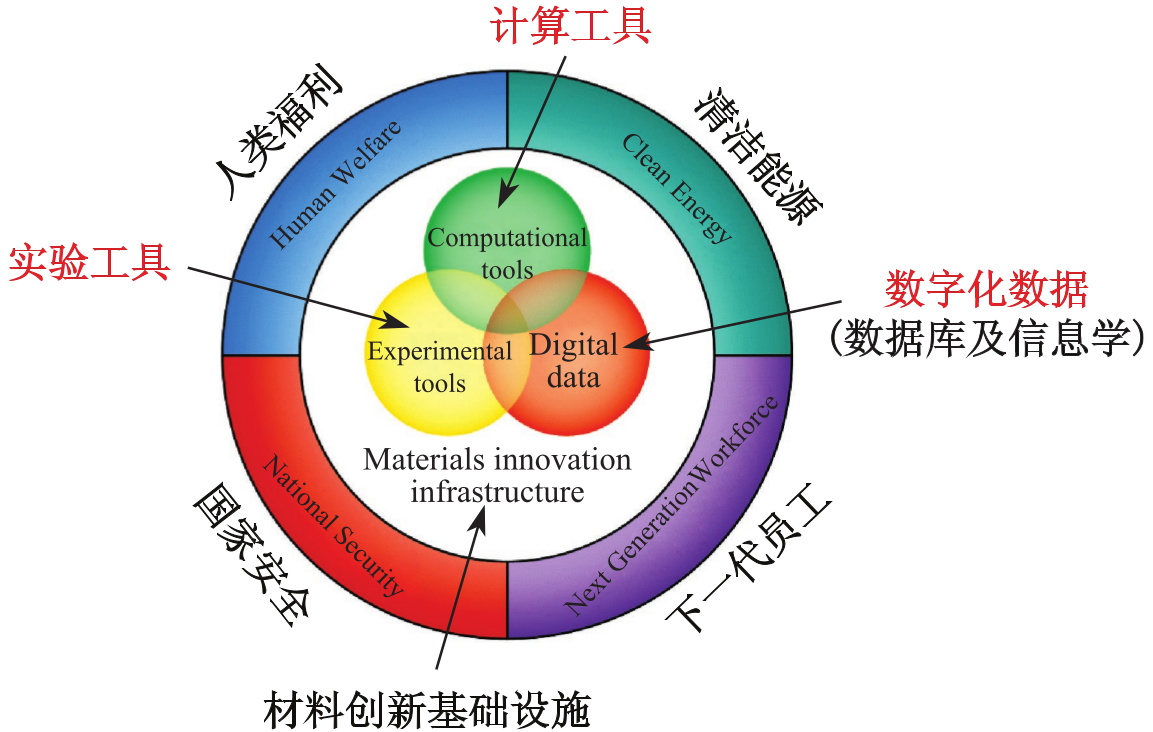
\includegraphics[height=2.55in,width=4.05in]{Figures/MGE.png}
%\caption{\tiny \textrm{Pseudopotential for metallic sodium, based on the empty core model and screened by the Thomas-Fermi dielectric function.}}%(与文献\cite{EPJB33-47_2003}图1对比)
%\caption{\tiny \textrm{Pseudopotential for metallic sodium, based on the empty core model and screened by the Thomas-Fermi dielectric function.}}%(与文献\cite{EPJB33-47_2003}图1对比)
\label{MGE}
\end{figure}
}

\frame
{
	\frametitle{材料模拟的基本思想和方法}
\begin{figure}[h!]
\vspace*{-0.25in}
\centering
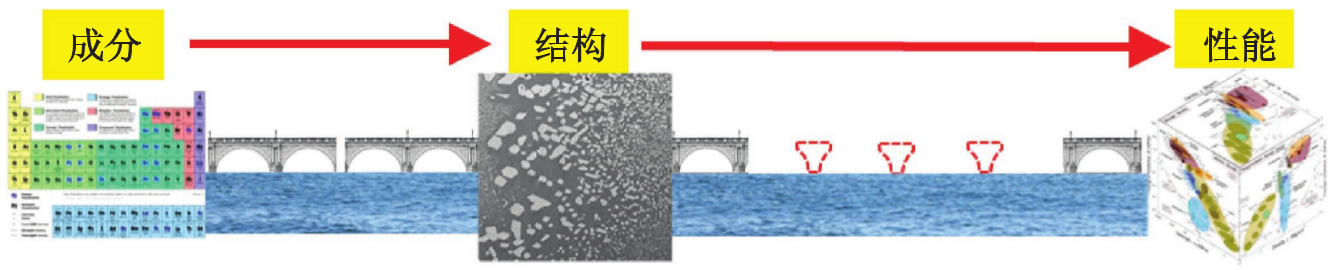
\includegraphics[height=0.80in,width=4.05in]{Figures/MGE-2.png}
%\caption{\tiny \textrm{Pseudopotential for metallic sodium, based on the empty core model and screened by the Thomas-Fermi dielectric function.}}%(与文献\cite{EPJB33-47_2003}图1对比)
\vskip 0.05pt
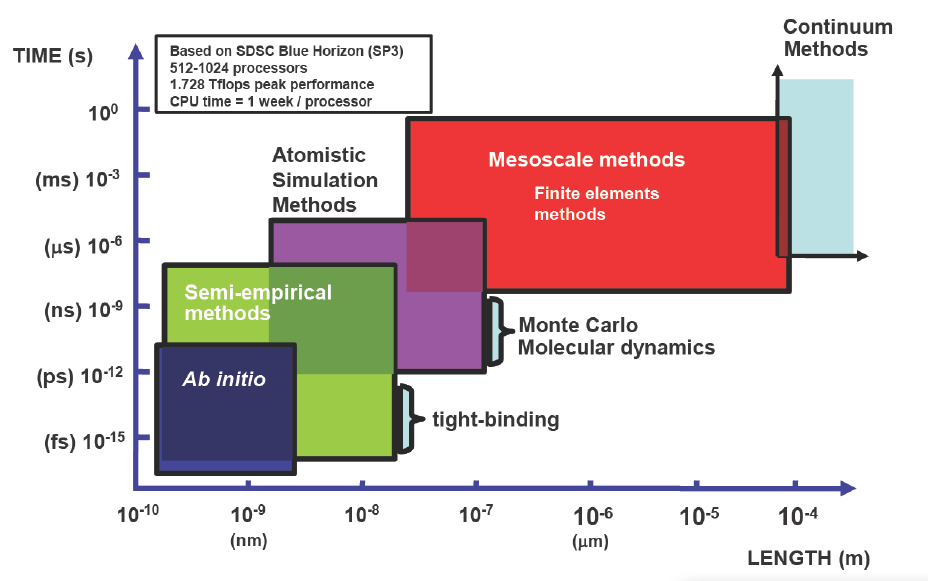
\includegraphics[height=2.20in,width=3.45in]{Figures/Multi-Scale-6.png}
%\caption{\tiny \textrm{Pseudopotential for metallic sodium, based on the empty core model and screened by the Thomas-Fermi dielectric function.}}%(与文献\cite{EPJB33-47_2003}图1对比)
\label{Multi-Scale}
\end{figure}
}

\frame
{
	\frametitle{\rm{I~Have~A~Dream}}
\begin{figure}[h!]
\vspace*{-0.18in}
\centering
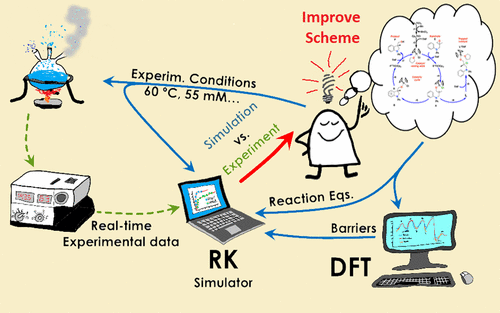
\includegraphics[height=2.55in,width=4.05in]{Figures/Schematic_Material-Design.png}
%\caption{\tiny \textrm{Pseudopotential for metallic sodium, based on the empty core model and screened by the Thomas-Fermi dielectric function.}}%(与文献\cite{EPJB33-47_2003}图1对比)
%\caption{\tiny \textrm{Pseudopotential for metallic sodium, based on the empty core model and screened by the Thomas-Fermi dielectric function.}}%(与文献\cite{EPJB33-47_2003}图1对比)
\label{Schematic_Material-Design}
\end{figure}
}

\section{量子力学基础}
\subsection{能量量子化}
\frame
{
	\frametitle{经典物理学天空的“两朵乌云”\textrm{(Dark Clouds)}}
\begin{figure}[h!]
\vspace*{-0.18in}
\centering
%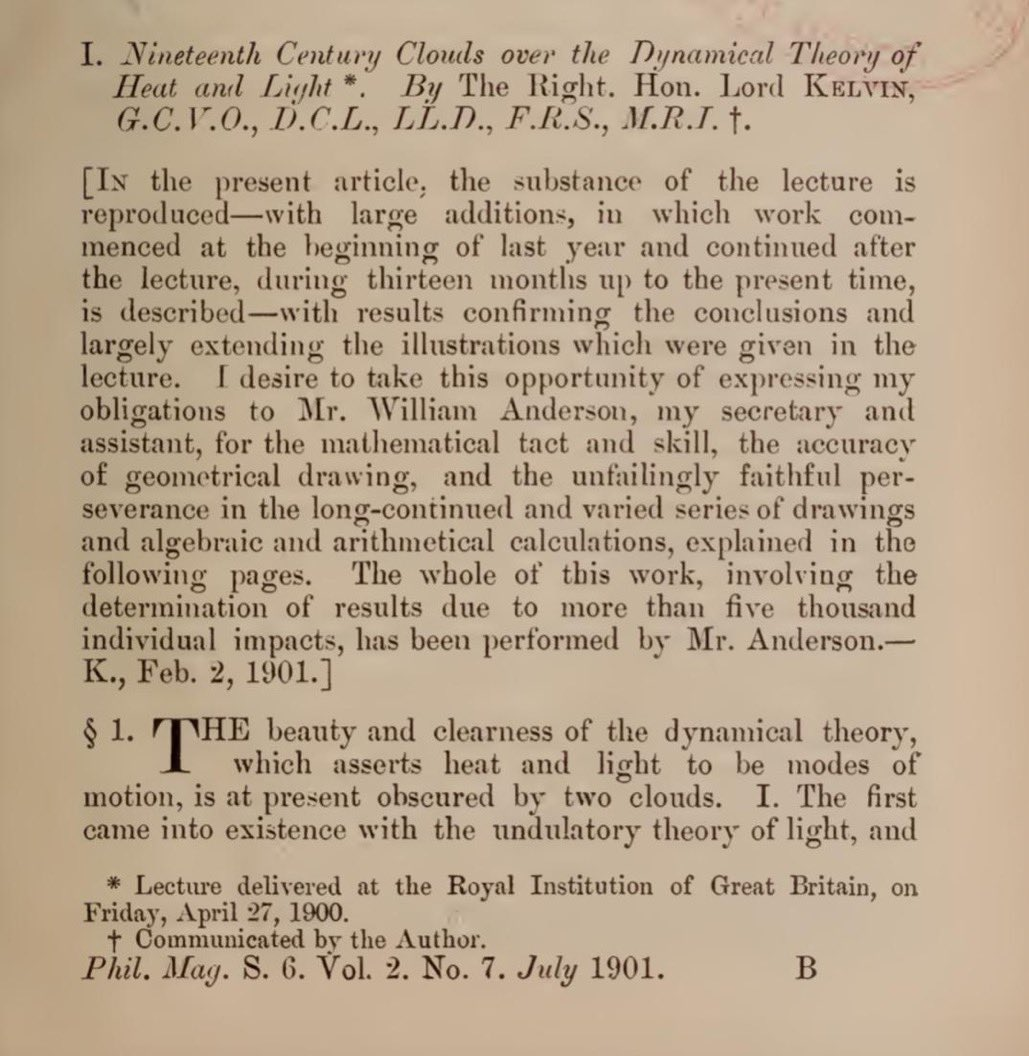
\includegraphics[height=2.90in,width=2.80in,viewport=0 0 1000 1100,clip]{Figures/Baron_Kelvin-Lecture.jpeg}
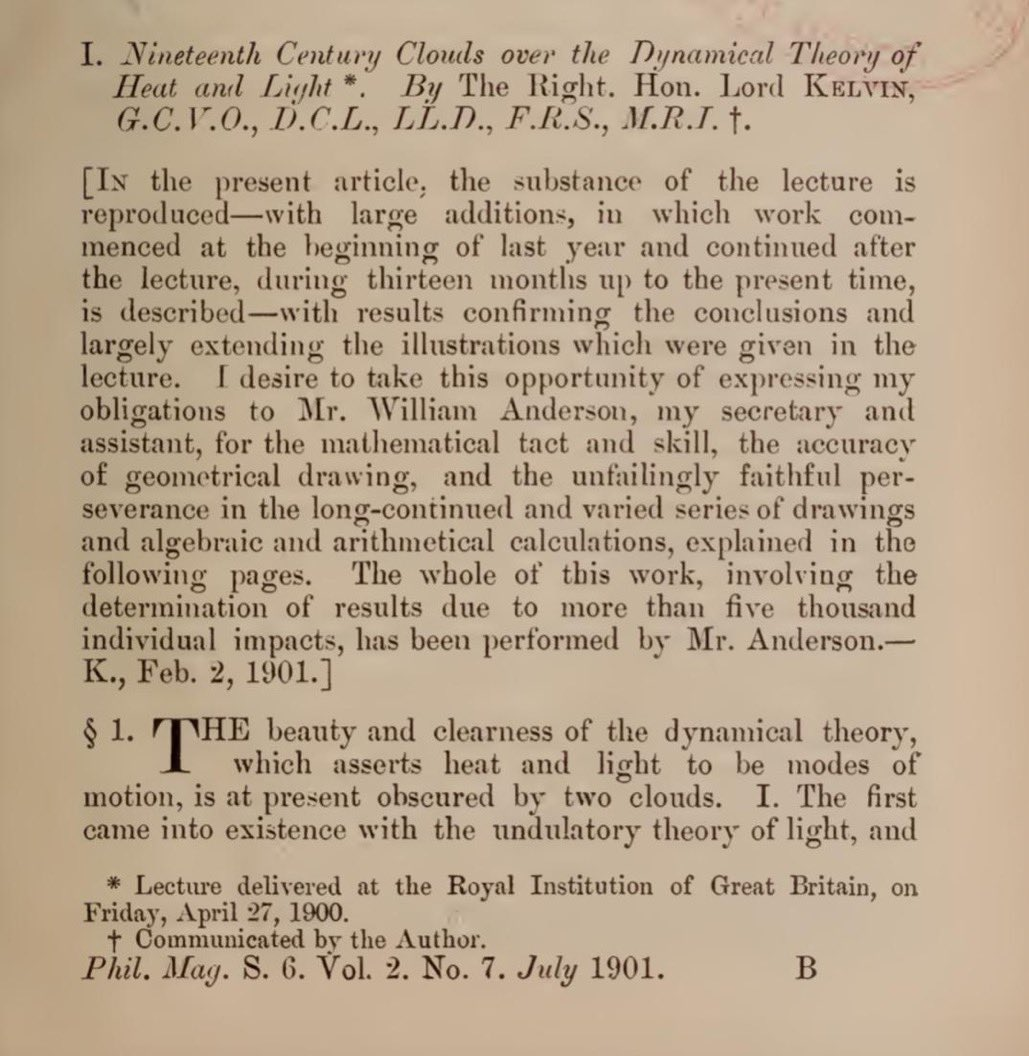
\includegraphics[height=0.35in,width=3.35in,viewport=0 900 1020 1030,clip]{Figures/Baron_Kelvin-Lecture.jpeg}
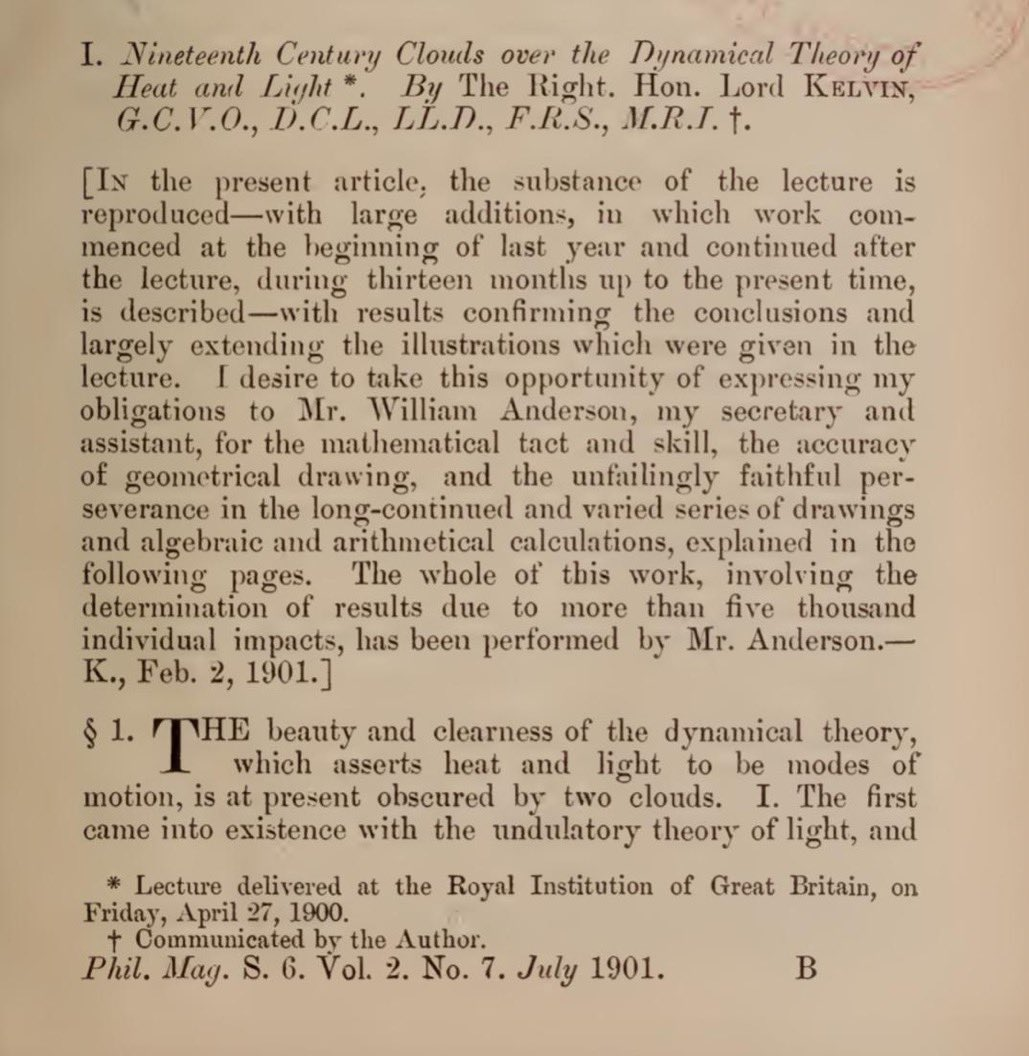
\includegraphics[height=0.80in,width=3.35in,viewport=0 50 1020 350,clip]{Figures/Baron_Kelvin-Lecture.jpeg}
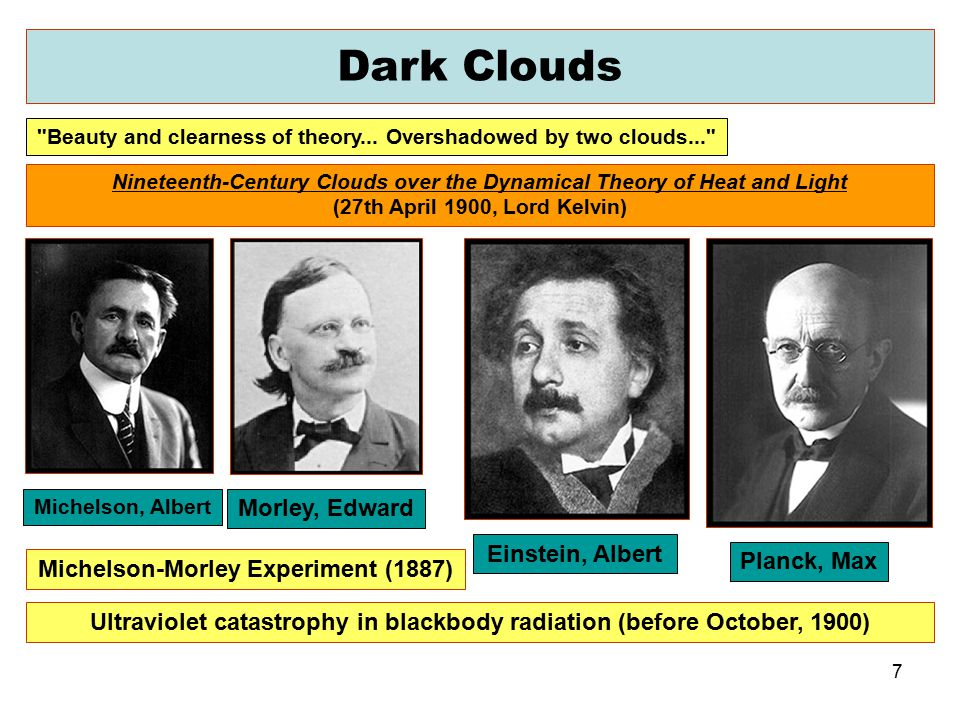
\includegraphics[height=1.85in,width=4.05in,viewport=0 50 735 370,clip]{Figures/Two-dark-cloud-in-physics-2.jpg}
\label{two_Dark_Clouds_2}
\end{figure}
}

%\frame
%{
%	\frametitle{经典物理学天空的“两朵乌云”\textrm{(Dark Clouds)}}
%\begin{figure}[h!]
%\vspace*{-0.18in}
%\centering
%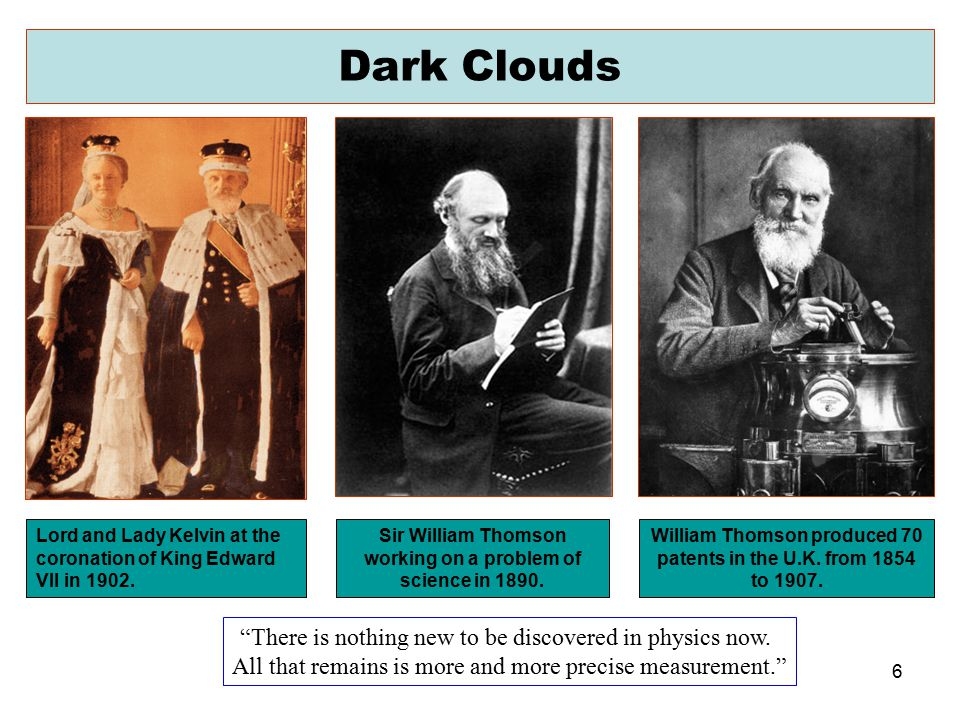
\includegraphics[height=2.50in,width=4.05in,viewport=0 20 735 470,clip]{Figures/Two-dark-cloud-in-physics-3.jpg}
%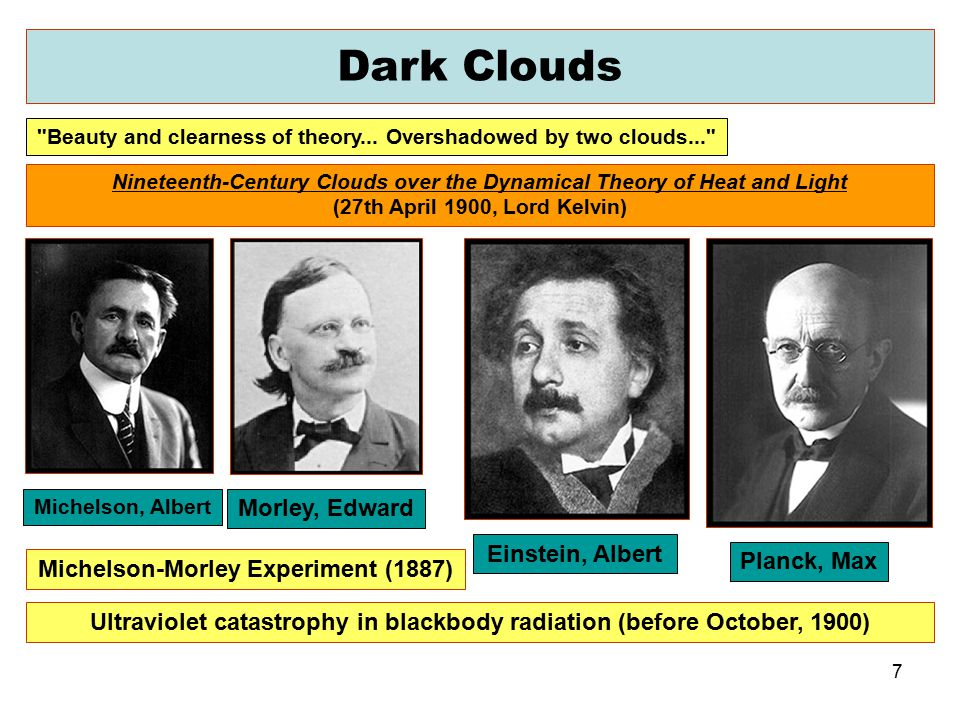
\includegraphics[height=2.40in,width=4.05in,viewport=0 50 735 470,clip]{Figures/Two-dark-cloud-in-physics-2.jpg}
%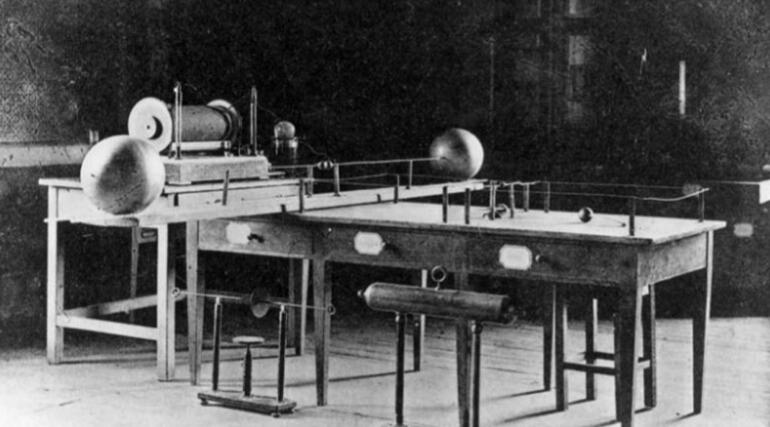
\includegraphics[height=2.40in,width=4.05in,viewport=0 0 580 325,clip]{Figures/Two-dark-cloud-in-physics-1.jpg}
%\label{two_Dark_Clouds_3}
%\end{figure}
%}
%
\frame
{
	\frametitle{黑体辐射与能量量子化}
	\textrm{1900}年,为了解释黑体辐射\textrm{(black-body radiation)}的能量密度与电磁辐射频率的关系,\textrm{M.~Planck}%放弃\textcolor{blue}{能量均分定理}\textrm{(the equipartition theorem)},
	引入\textcolor{red}{能量量子化}\textrm{(quantization of energy)}的假设,利用统计物理推导出与实验符合得非常好的黑体辐射\textrm{Planck~}公式:~
	\begin{displaymath}
		\rho_{\nu}\mathrm{d}{\nu}=\dfrac{8{\pi}h{\nu}^3}{C^2}\bigg(\dfrac1{\mathrm{e}^{h\nu/kT}-1}\bigg)\mathrm{d}\nu
	\end{displaymath}
\begin{figure}[h!]
\centering
\vspace{-10.5pt}
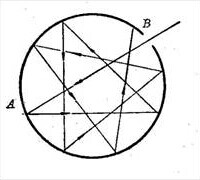
\includegraphics[height=1.45in,width=1.45in,viewport=0 0 136 136,clip]{Figures/Black_box.jpg}
\hskip 1pt
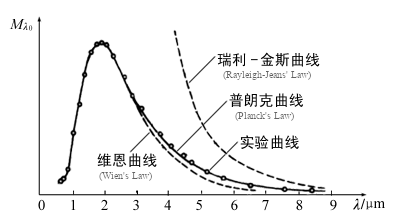
\includegraphics[height=1.32in,width=2.25in,viewport=0 0 390 215,clip]{Figures/Black_box_curve.png}
\caption{\textrm{The black-body radiation and the curve}}
\label{Black_box}
\end{figure}
}

\frame
{
	\frametitle{波-粒二象性与光电效应}
\begin{figure}[h!]
\centering
\vspace{-15.5pt}
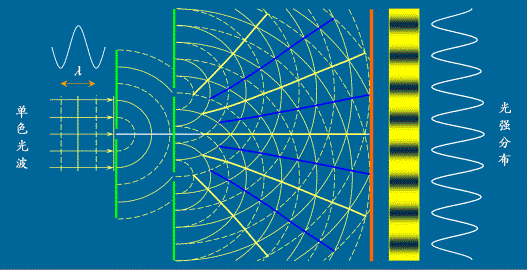
\includegraphics[height=1.35in,width=2.70in,viewport=0 0 536 280,clip]{Figures/wave-particle_duality.png}
\vskip 1pt
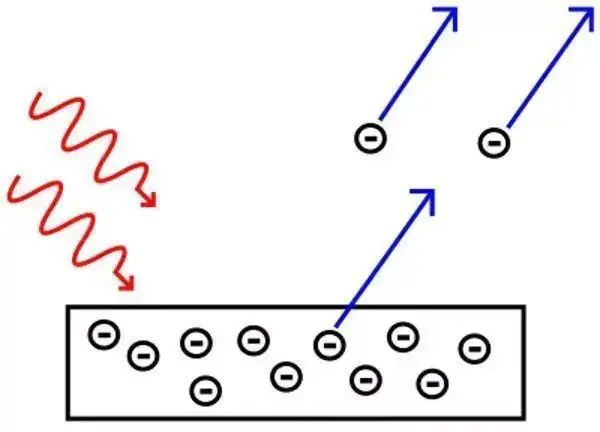
\includegraphics[height=1.32in,width=2.05in,viewport=0 0 620 455,clip]{Figures/Photoelectic_effect.png}
\caption{\textrm{The wave-particle duality and Photoelectric effect}}
\label{wave_and_particle}
\end{figure}
}

\frame
{
	\frametitle{电子衍射、\textrm{Compton~effect}与\textrm{H}原子光谱}
\begin{figure}[h!]
\centering
\vspace{-15.5pt}
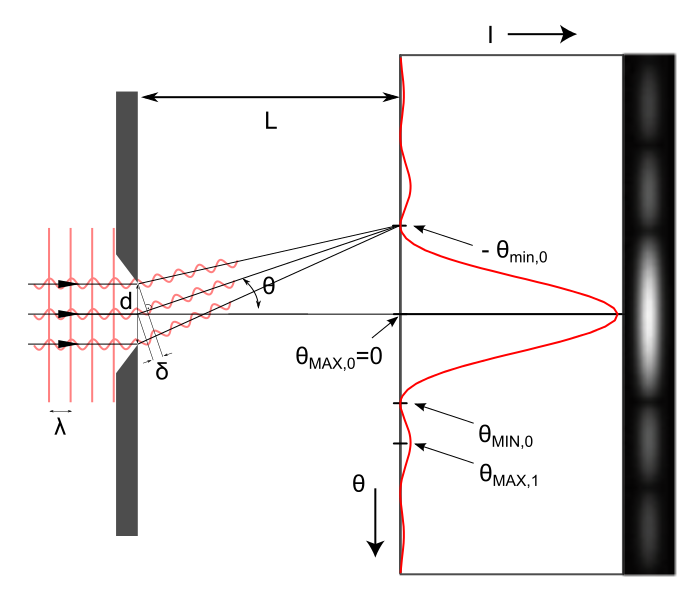
\includegraphics[height=1.35in,width=1.80in,viewport=0 0 680 600,clip]{Figures/Single_Slit_Diffraction.png}
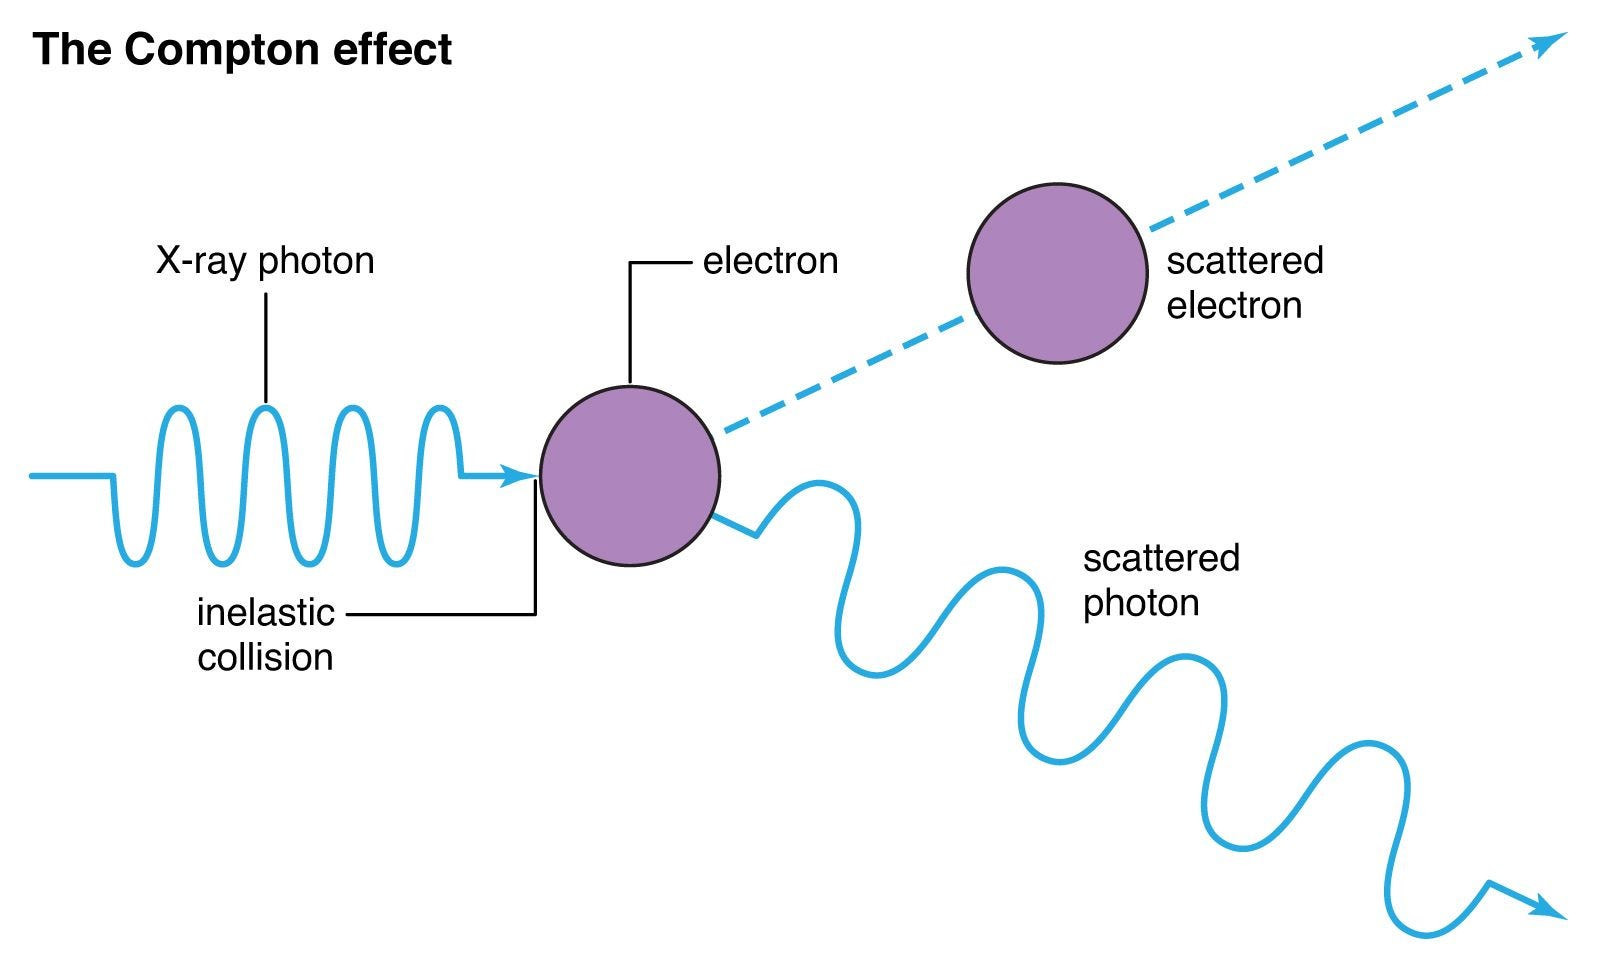
\includegraphics[height=1.20in,width=2.10in,viewport=0 0 1600 950,clip]{Figures/Compton_effect.jpg}\\
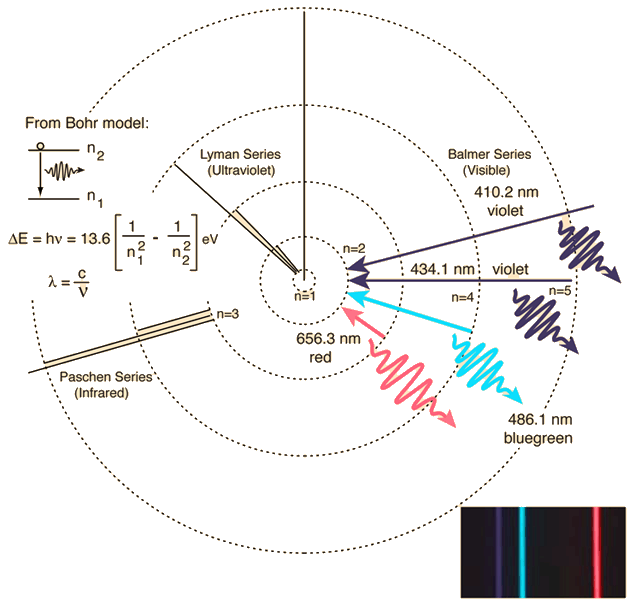
\includegraphics[height=1.65in,width=1.75in,viewport=0 0 620 600,clip]{Figures/Hydrogen_spectrum-3.png}
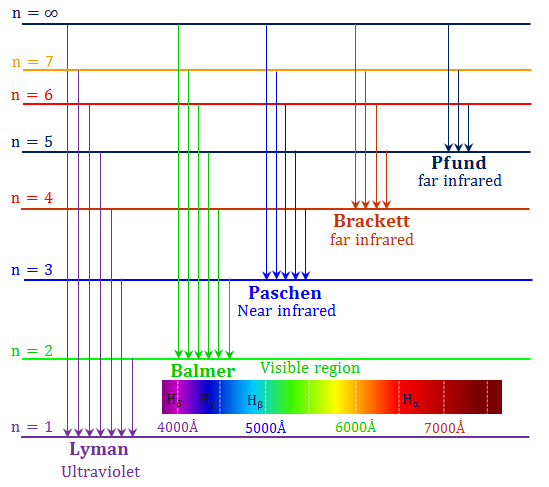
\includegraphics[height=1.55in,width=1.75in,viewport=0 0 500 380,clip]{Figures/Hydrogen_spectrum-2.png}
%\caption{\textrm{The wave-particle duality and Photoelectric effect}}
\label{electron:wave_and_particle}
\end{figure}
}

\subsection{\textrm{Schr\"odinger}方程与量子力学的建立}
\frame
{
	\frametitle{\textrm{De Broglie}物质波}
\begin{minipage}{0.53\textwidth}
\begin{figure}[h!]
\centering
\vspace{-15.5pt}
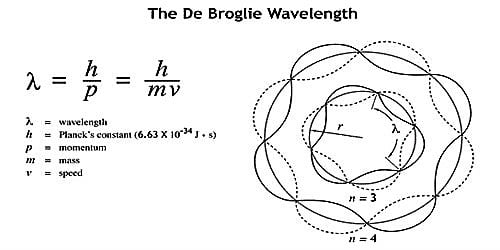
\includegraphics[height=1.3in,width=2.1in,viewport=0 0 500 280,clip]{Figures/De-Broglie-waves.jpg}
%\caption{\textrm{The wave-particle duality and Photoelectric effect}}
\label{Matter_wave}
\end{figure}
经典的观念:
\begin{itemize}
	\item \textcolor{red}{粒子}:~\textcolor{blue}{物质存在的形式}
	\item \textcolor{red}{波动}:~\textcolor{blue}{能量传递的形式}
\end{itemize}
\end{minipage}
\begin{minipage}{0.45\textwidth}
\begin{figure}[h!]
\centering
\vspace{-15.5pt}
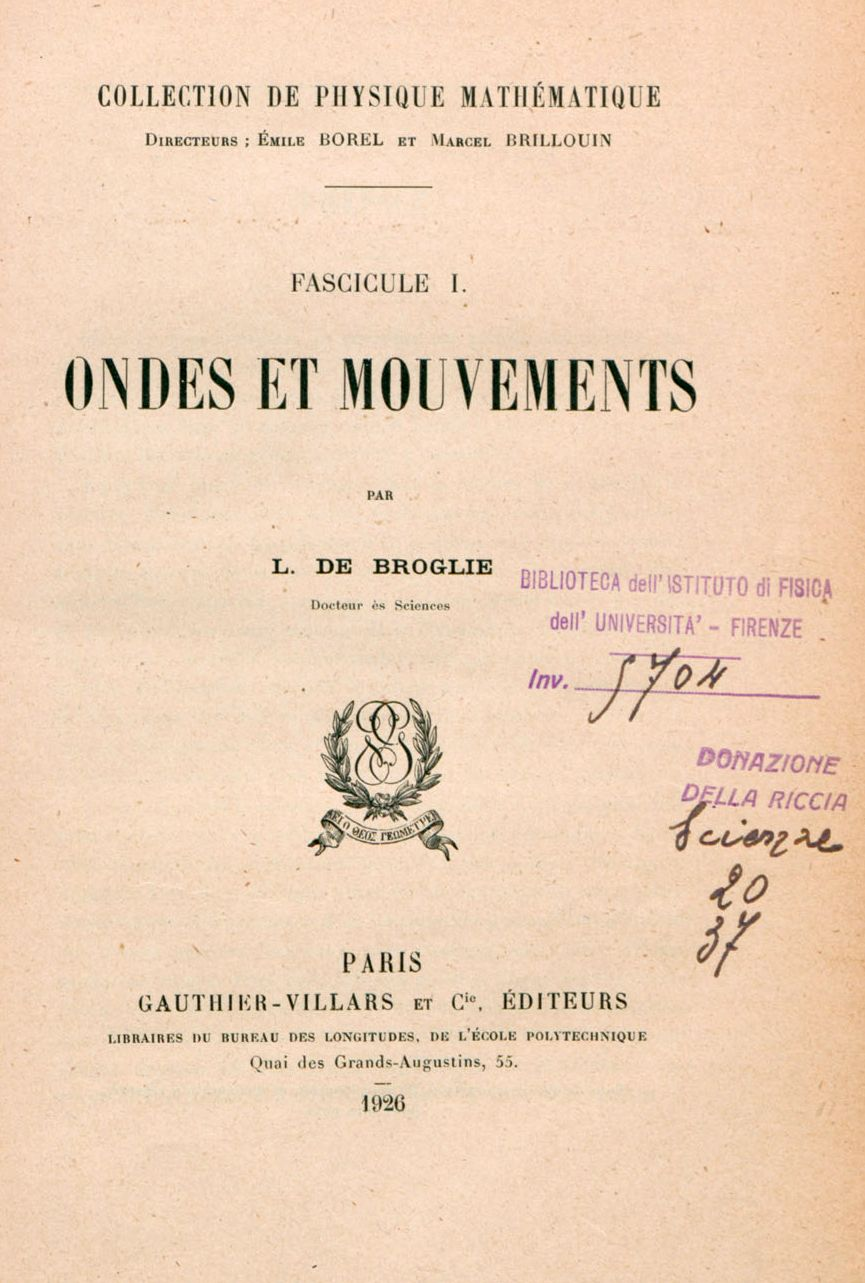
\includegraphics[height=2.80in,width=1.90in,viewport=0 0 430 650,clip]{Figures/De_Broglie-dissertation_Cover.jpg}
%\caption{\textrm{The wave-particle duality and Photoelectric effect}}
\label{De_Broglie-dissertation}
\end{figure}
\end{minipage}
}

\frame
{
	\frametitle{经典力学\textrm{Classical Mechanics}}
\begin{figure}[h!]
\vspace*{-0.18in}
\centering
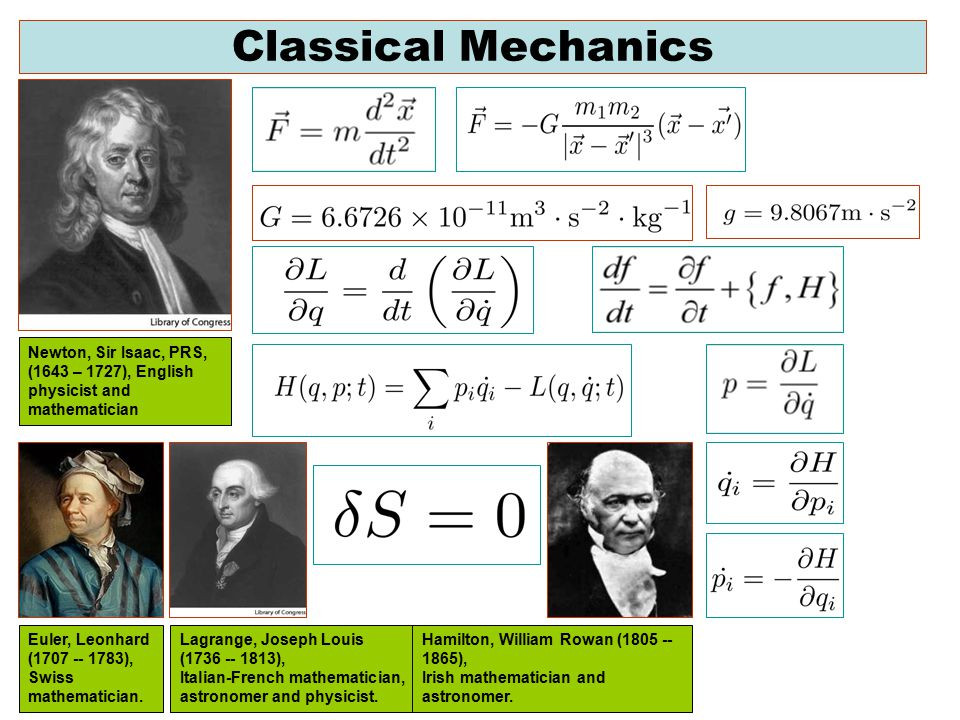
\includegraphics[height=2.65in,width=4.05in,viewport=0 0 715 495,clip]{Figures/Classical_Mechanics.jpg}
%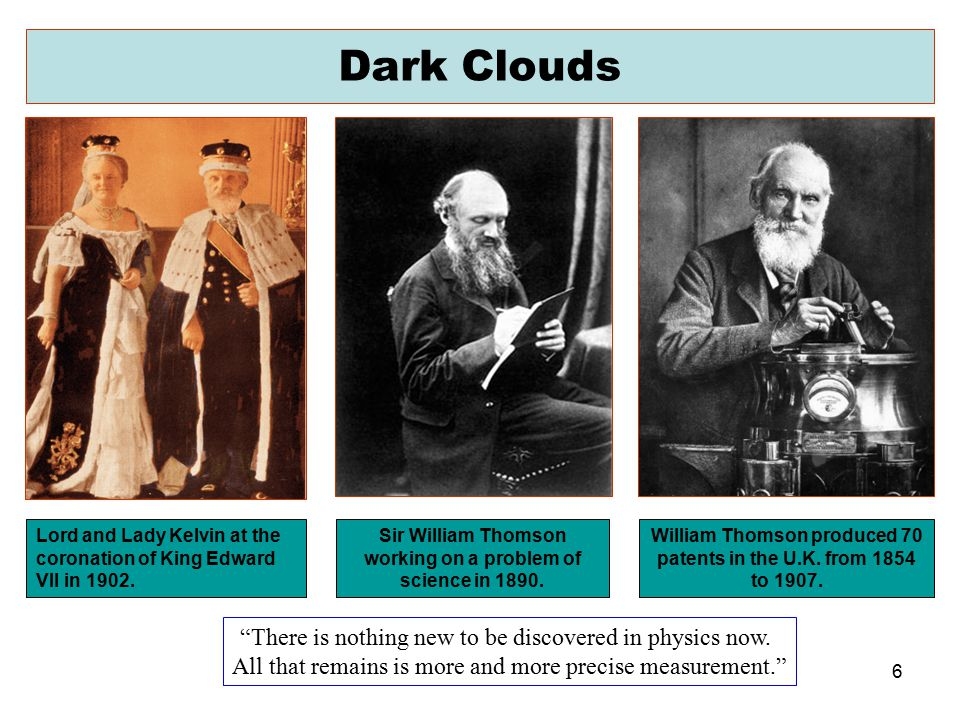
\includegraphics[height=2.50in,width=4.05in,viewport=0 20 735 470,clip]{Figures/Two-dark-cloud-in-physics-3.jpg}
%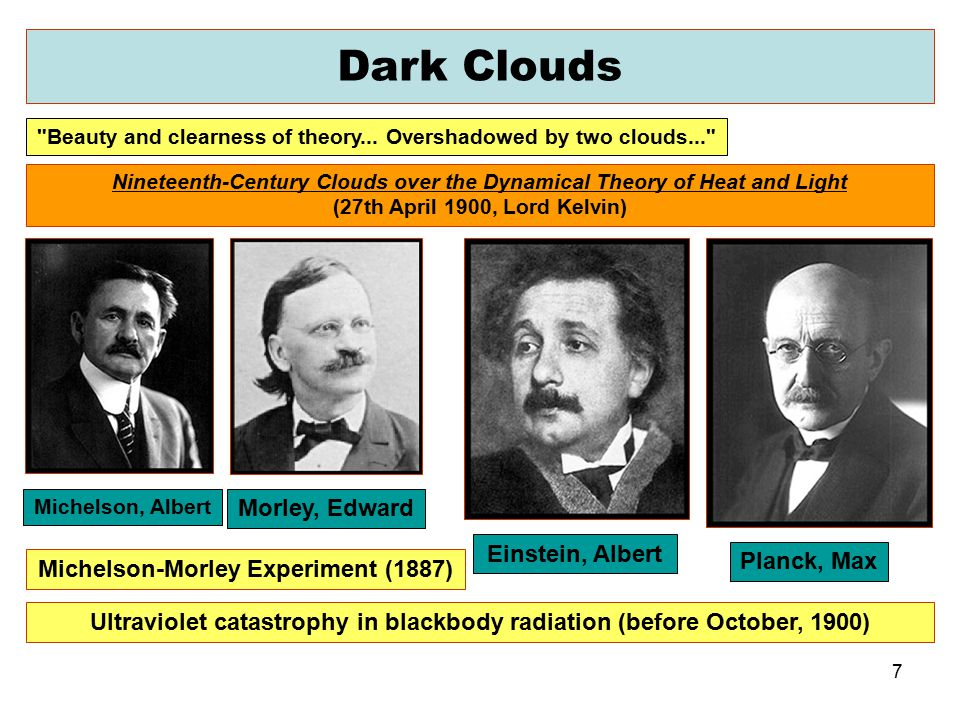
\includegraphics[height=2.40in,width=4.05in,viewport=0 50 735 470,clip]{Figures/Two-dark-cloud-in-physics-2.jpg}
%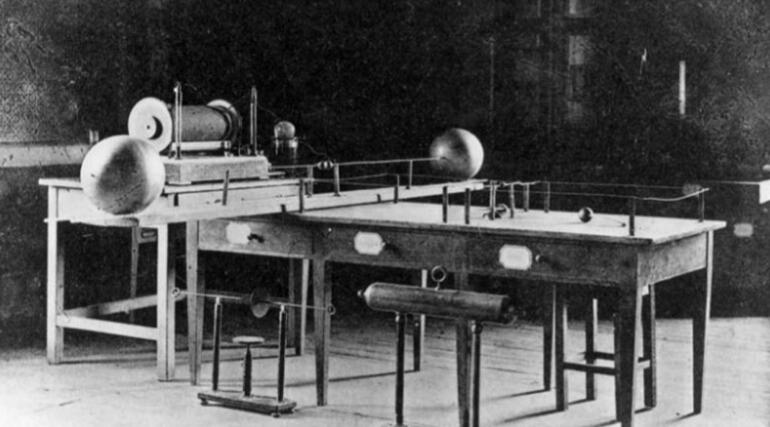
\includegraphics[height=2.40in,width=4.05in,viewport=0 0 580 325,clip]{Figures/Two-dark-cloud-in-physics-1.jpg}
\label{Classical_Mechanics}
\end{figure}
}

\frame
{
	\frametitle{\textrm{\small Newtonian, Lagrangian and Hamiltonian Mechanics}}
	\begin{itemize}
   		\setlength{\itemsep}{10pt}
		\item \textrm{\textcolor{blue}{Newtonian~Mechanics}}\\
		牛顿运动定律体系是以力、加速度、动量这些矢量为基本量来描述力学系统在欧氏空间的运动~(用几何方程表述约束)
	\item \textrm{\textcolor{blue}{Lagrangian~Mechanics}}\\
		拉格朗日力学是关于研究对象在其对应的约束系统下的运动形式,大大压缩牛顿方程描述需要的约束个数。不需要在另外设未知数目
	\item \textrm{\textcolor{blue}{Hamiltonian~Mechanics}}\\
		哈密度力学由拉格朗日力学演变而来,把位置和动量彻底分开,成为两种独立变量,由此诞生相空间。把广义动量和广义坐标放在等同的位置上(正则配对,方程降阶)
		\vskip 6pt
		拉格朗日力学和哈密顿力学的基本量是\textcolor{blue}{系统的能量}等标量,通过变分原理建立系统的动力学方程,所以拉格朗日力学和哈密顿力学合称\textcolor{magenta}{分析力学}
	\end{itemize}
}

\frame
{
	\frametitle{\textrm{Invariante Variationsprobleme}}
\begin{figure}[h!]
\centering
%
\vspace{-10.5pt}
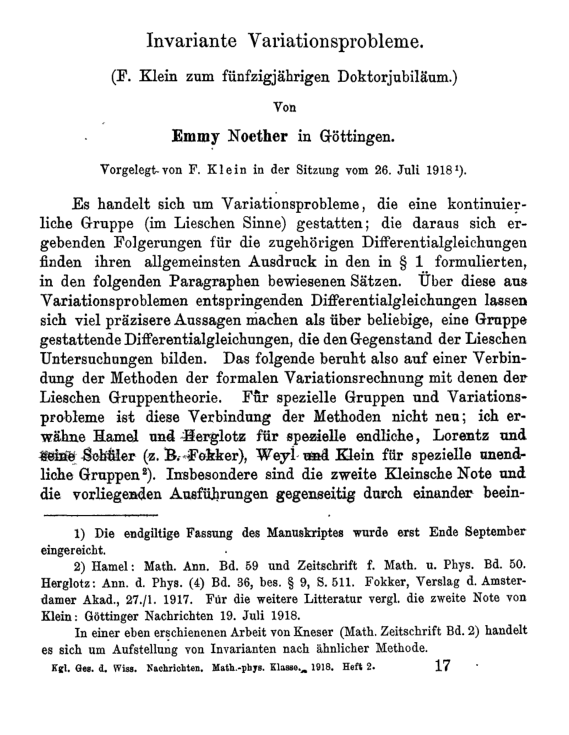
\includegraphics[height=0.52\textwidth,width=0.42\textwidth,viewport=0 0 450 580,clip]{Figures/Noether_theorem-1st_page.png}
\label{Noether_theorem}
\end{figure}
\begin{itemize}
\centering
	\item \textcolor{red}{能量守恒}~$\Longleftrightarrow$~\textcolor{magenta}{时间平移对称性}
	\item \textcolor{red}{动量守恒}~$\Longleftrightarrow$~\textcolor{magenta}{空间平移对称性}
	\item \textcolor{red}{角动量守恒}~$\Longleftrightarrow$~\textcolor{magenta}{空间旋转对称性}
\end{itemize}
}

\frame
{
	\frametitle{\textrm{驻波}}
\begin{figure}[h!]
\centering
\vspace{-15.5pt}
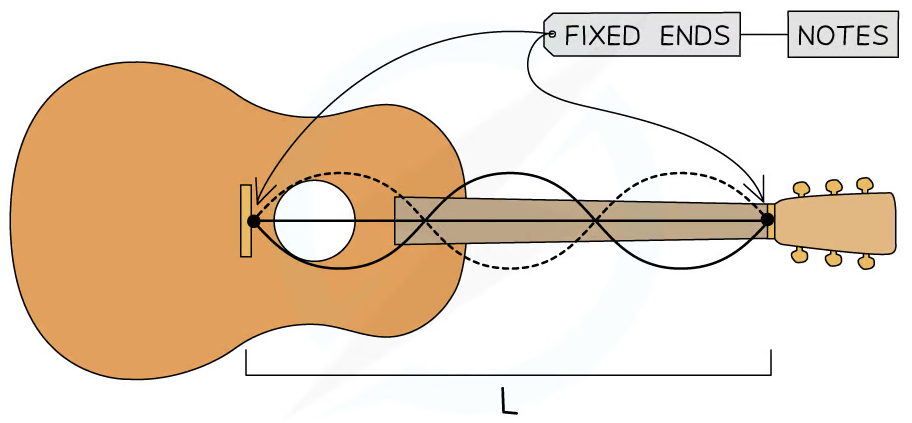
\includegraphics[height=0.40\textwidth,width=0.8\textwidth,viewport=0 0 900 450,clip]{Figures/Guitar-string.png}
\vskip 0.1pt
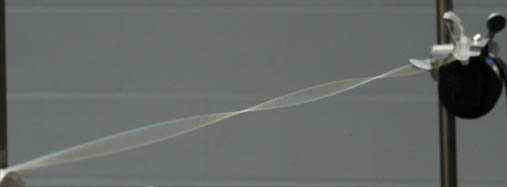
\includegraphics[height=0.35\textwidth,width=0.8\textwidth,viewport=0 0 122 48,clip]{Figures/string-standing-wave.jpg}
%\caption{\textrm{ABINIT}的Si.in}
\label{Standing_Wave_0}
\end{figure}
}

\frame
{
	\frametitle{驻波方程与势阱}
\begin{figure}[h!]
\centering
\vspace{-12.5pt}
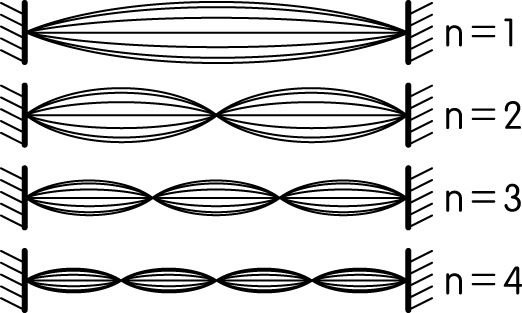
\includegraphics[height=0.32\textwidth,width=0.7\textwidth,viewport=0 0 125 75,clip]{Figures/Standing_wave.jpeg}
\vskip 2pt
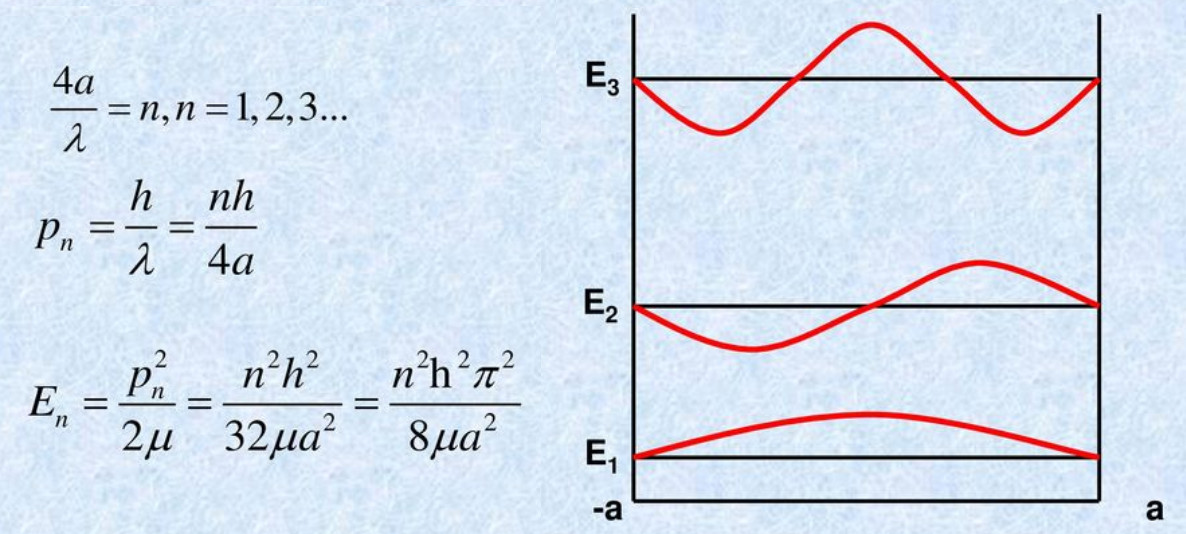
\includegraphics[height=0.40\textwidth,width=0.9\textwidth,viewport=0 0 1200 550,clip]{Figures/Standing_wave-energy.jpg}
%\caption{\textrm{ABINIT}的Si.in}
\label{Standing_Wave_1}
\end{figure}
}

\frame
{
	\frametitle{驻波方程与势阱}
\begin{figure}[h!]
\centering
\vspace{-5.5pt}
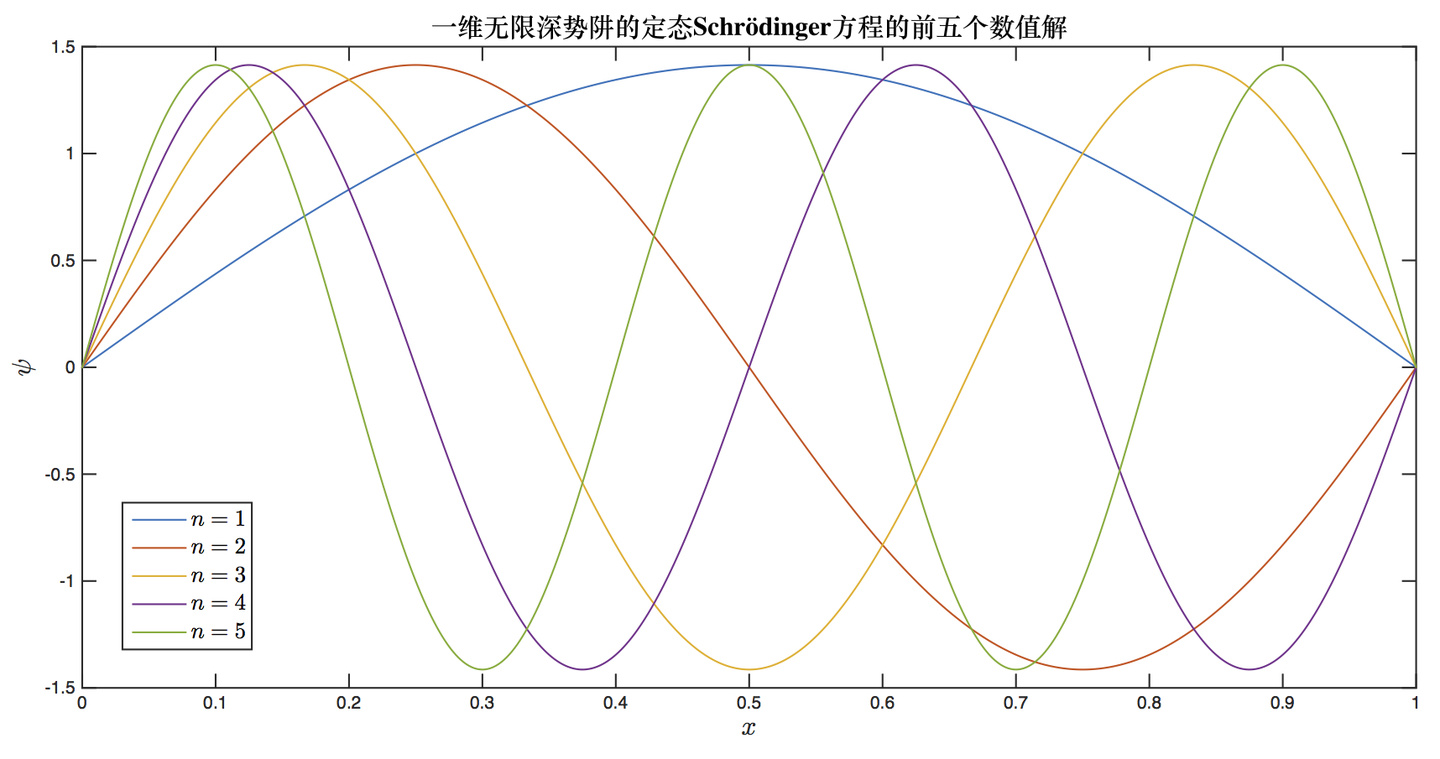
\includegraphics[height=0.55\textwidth,width=1.0\textwidth,viewport=0 0 720 400,clip]{Figures/Standing_wave-energy_1-5.jpg}
%\caption{\textrm{ABINIT}的Si.in}
\label{Standing_Wave_2}
\end{figure}
}

\frame
{
	\frametitle{驻波方程与势阱}
\begin{figure}[h!]
\centering
\vspace{-0.5pt}
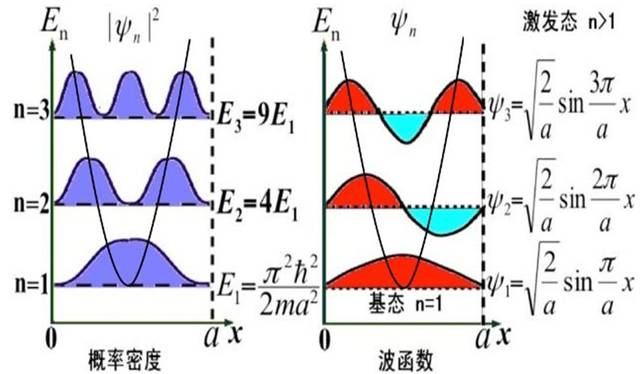
\includegraphics[height=0.46\textwidth,width=1.0\textwidth,viewport=0 0 650 390,clip]{Figures/Standing_wave_Energy.jpeg}
%\caption{\textrm{ABINIT}的Si.in}
\label{Standing_Wave_3}
\end{figure}
}

\frame
{
	\frametitle{原子中电子的驻波方程}
\begin{figure}[h!]
	\vspace{-10.5pt}
\centering
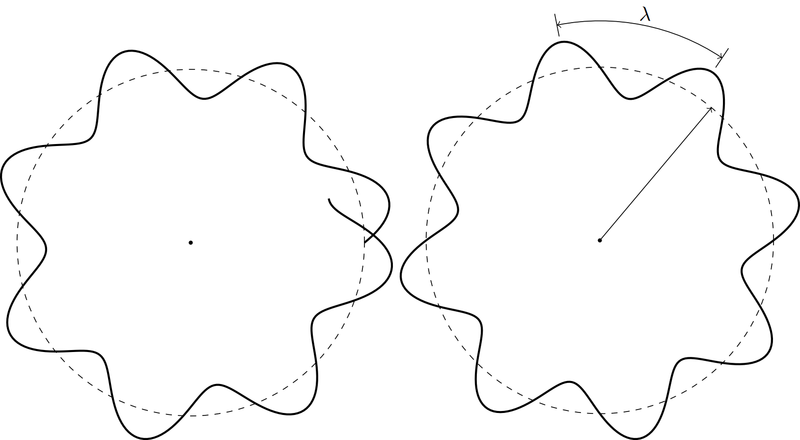
\includegraphics[height=0.38\textwidth,width=0.74\textwidth,viewport=0 0 840 440,clip]{Figures/Standing_wave-atom.png}
\vskip 2pt
\animategraphics[autoplay, loop, height=1.3in]{1}{Figures/Standing_wave_circle_}{1}{25}
\label{Atomic-electron_Standing_wave}
\end{figure}
}

\frame
{
	\frametitle{原子中的电子轨道和能量}
\begin{minipage}{0.43\textwidth}
\begin{figure}[h!]
%	\vspace{-14.8pt}
	\vspace{-4.8pt}
\centering
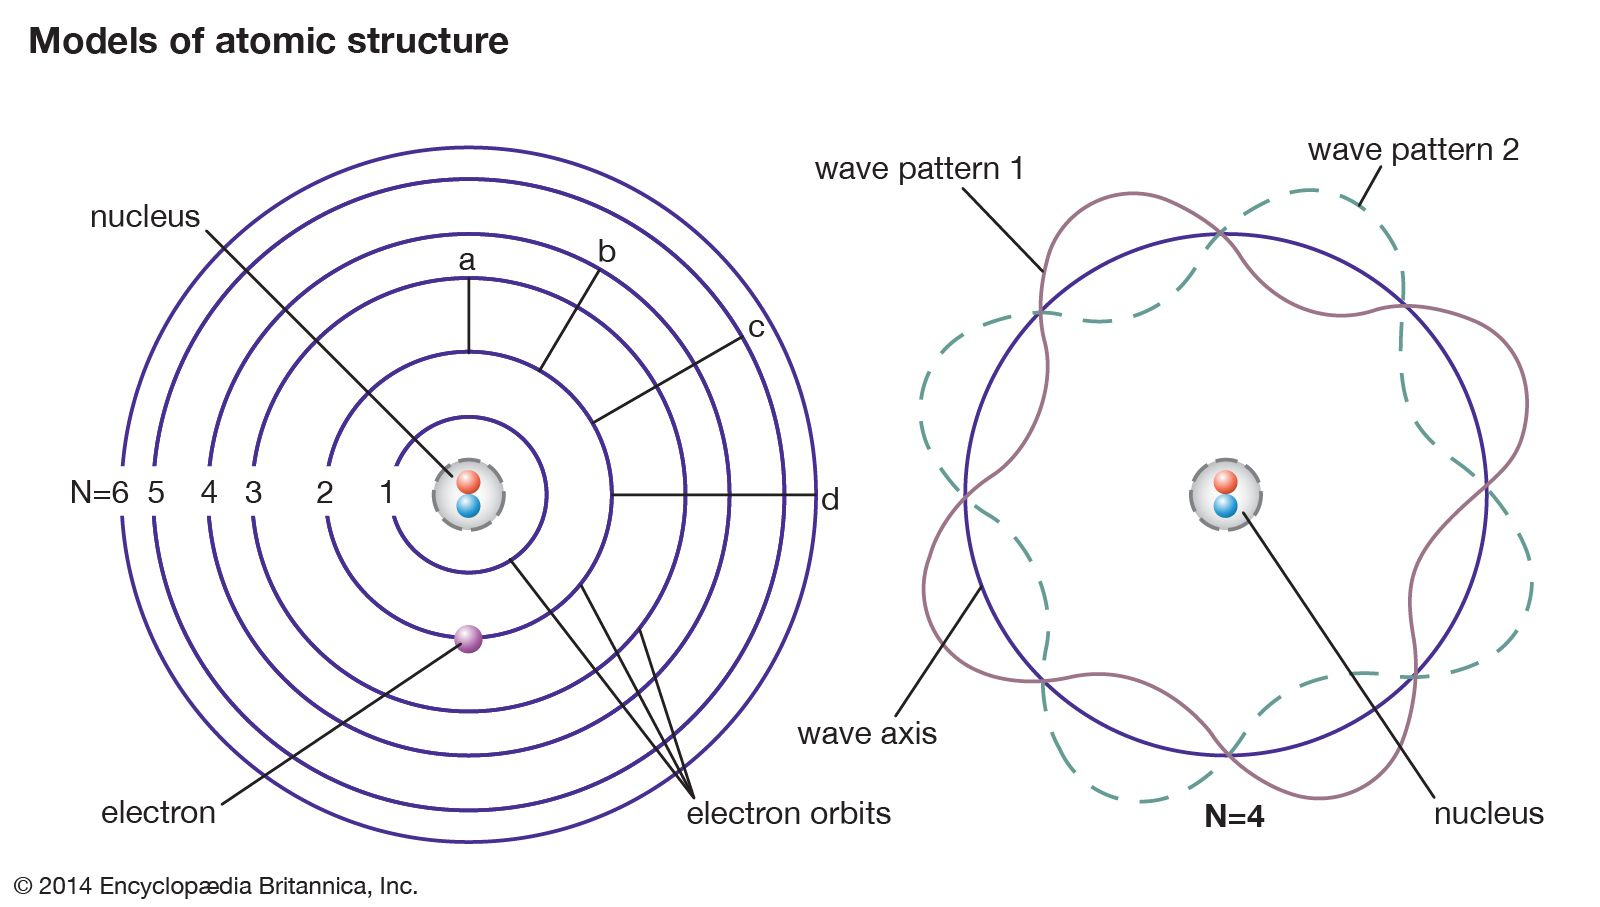
\includegraphics[height=0.57\textwidth,width=1.00\textwidth,viewport=0 50 1680 1000,clip]{Figures/electron-theory-Bohr-point-mass-energy-levels.jpg}
%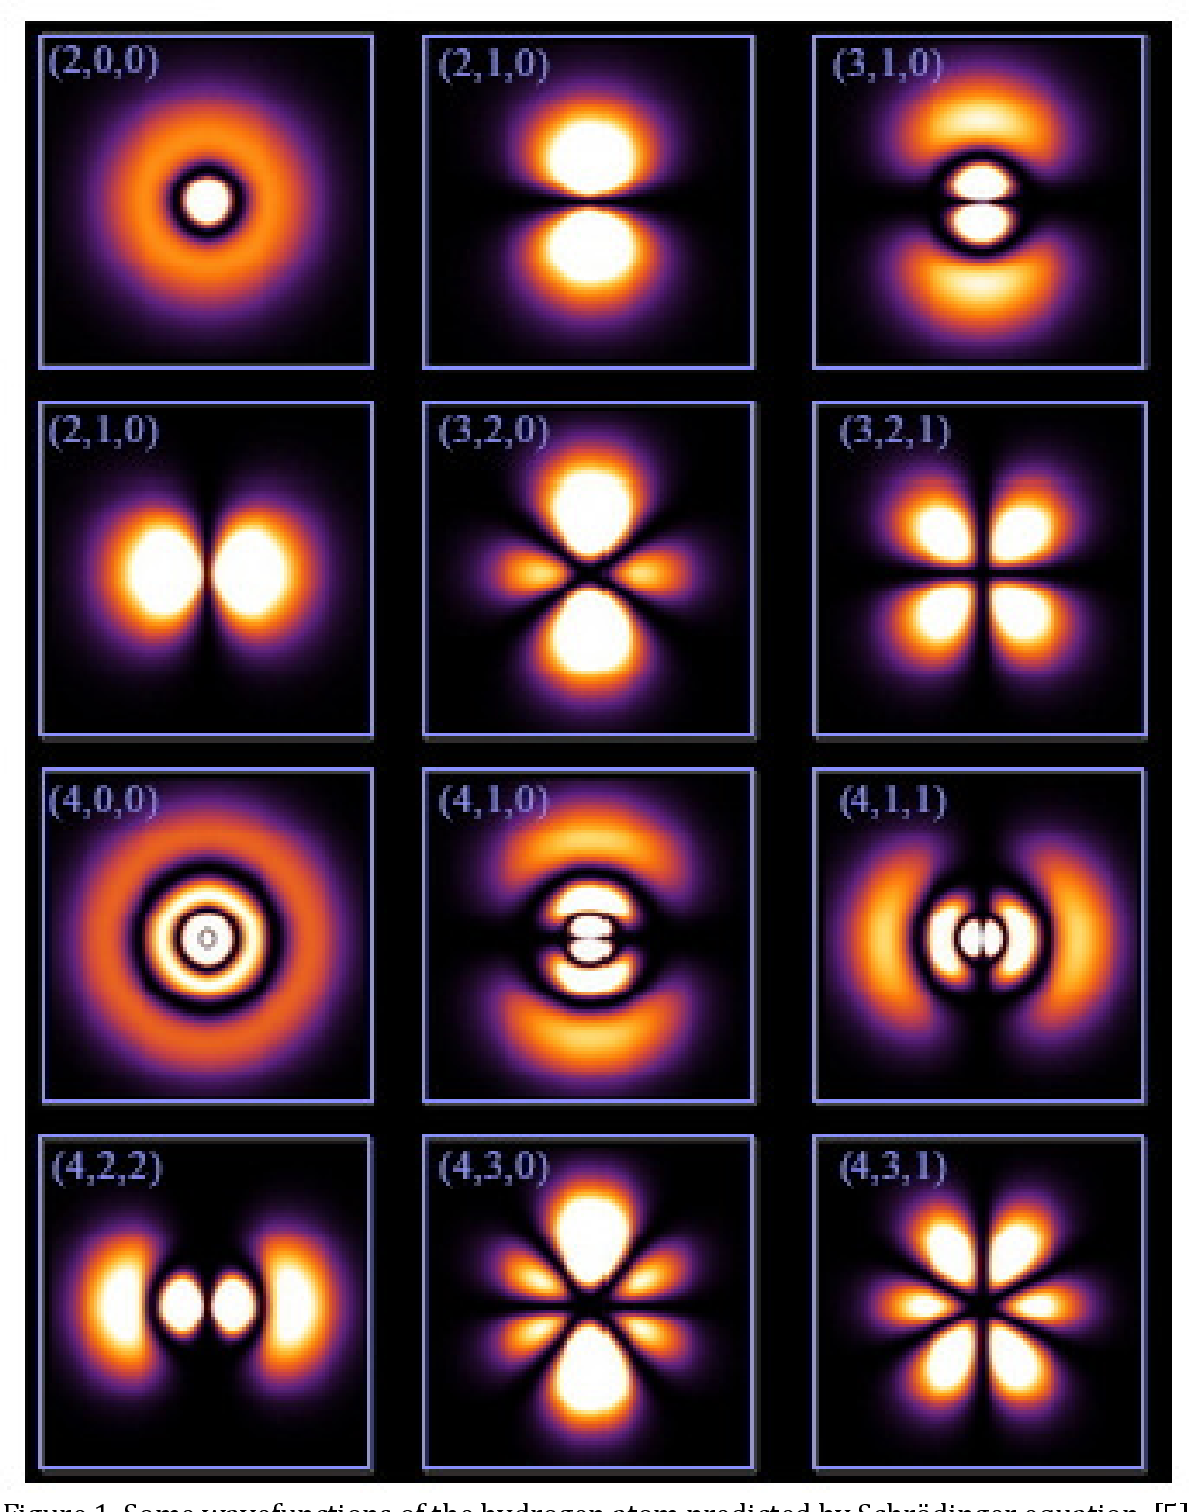
\includegraphics[height=1.23\textwidth,width=1.00\textwidth,viewport=0 10 1250 1500,clip]{Figures/wave_function.png}
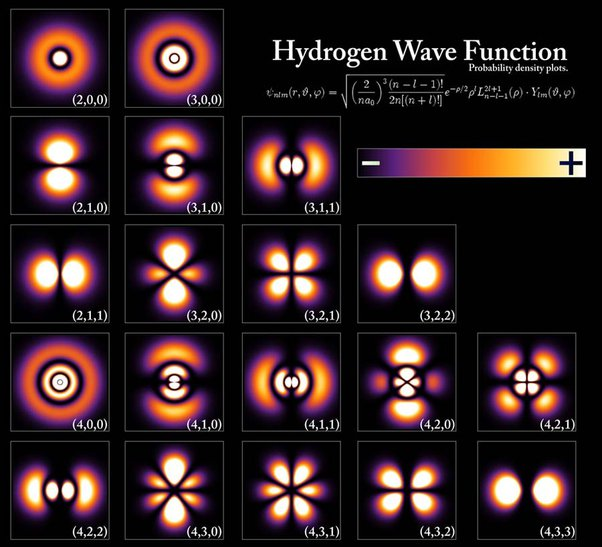
\includegraphics[height=0.95\textwidth,width=1.00\textwidth,viewport=0 0 630 650,clip]{Figures/wave_function-2.jpeg}
\label{Atomic-electron_wave}
\end{figure}
\end{minipage}
\begin{minipage}{0.55\textwidth}
\begin{figure}[h!]
	\vspace{-16.5pt}
\centering
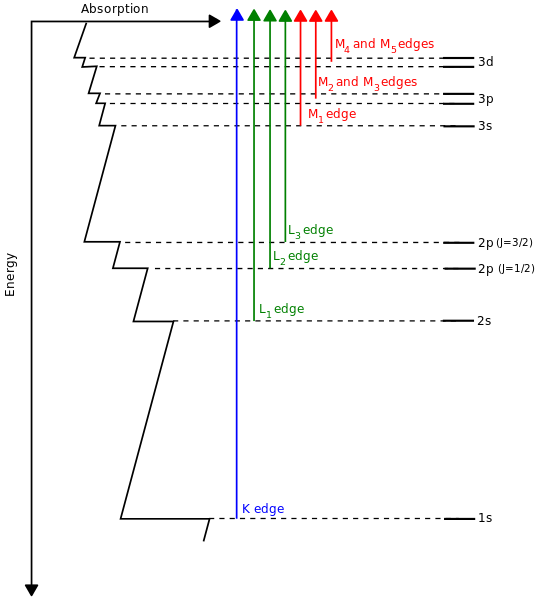
\includegraphics[height=1.10\textwidth,width=1.00\textwidth,viewport=0 0 560 600,clip]{Figures/Electron_orbital-energy.png}
\label{Atomic-electron_wave-energy}
\end{figure}
\end{minipage}
}

\frame
{
	\frametitle{\textrm{Schr\"odinger}~方程}
\begin{minipage}{0.49\textwidth}
\begin{figure}[h!]
\centering
%
\vspace{-25.5pt}
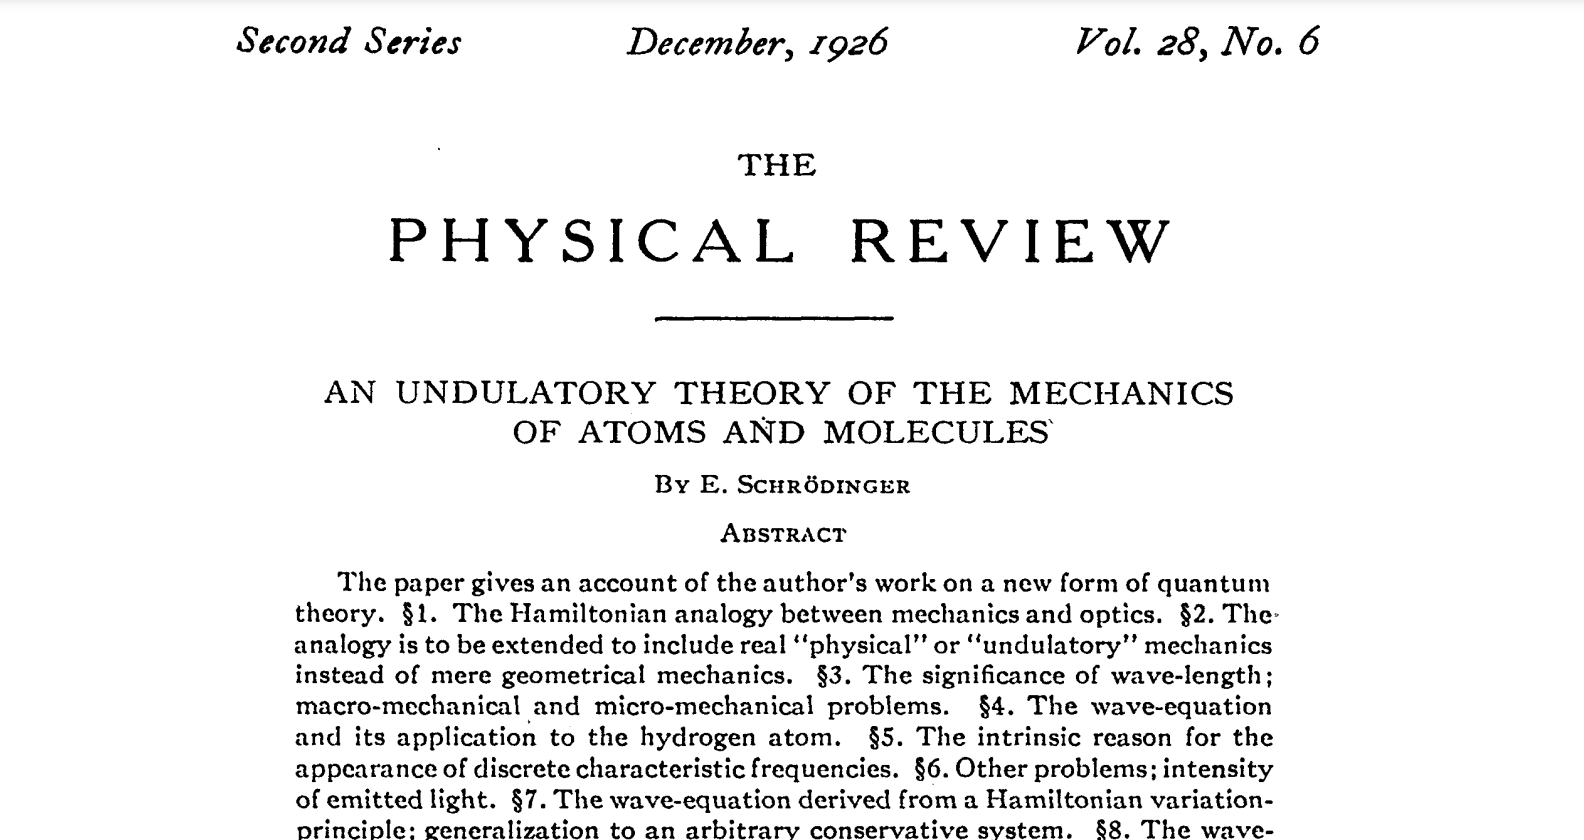
\includegraphics[height=1.80in,width=2.00in,viewport=180 0 1380 1100,clip]{Figures/Schrodinger_article.png}
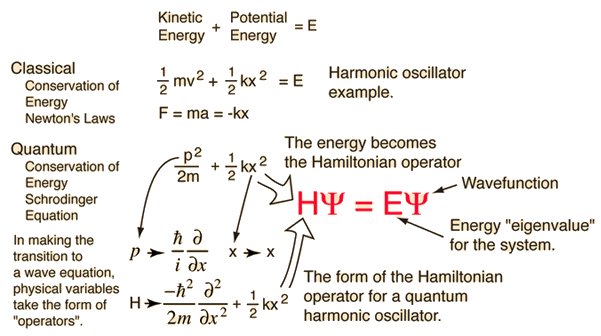
\includegraphics[height=1.20in,width=2.00in,viewport=0 0 600 350,clip]{Figures/Schrodinger_Equation.png}
\label{Schrodinger_Equation}
\end{figure}
\end{minipage}
\begin{minipage}{0.49\textwidth}
\begin{figure}[h!]
\centering
%
\vspace{-15.5pt}
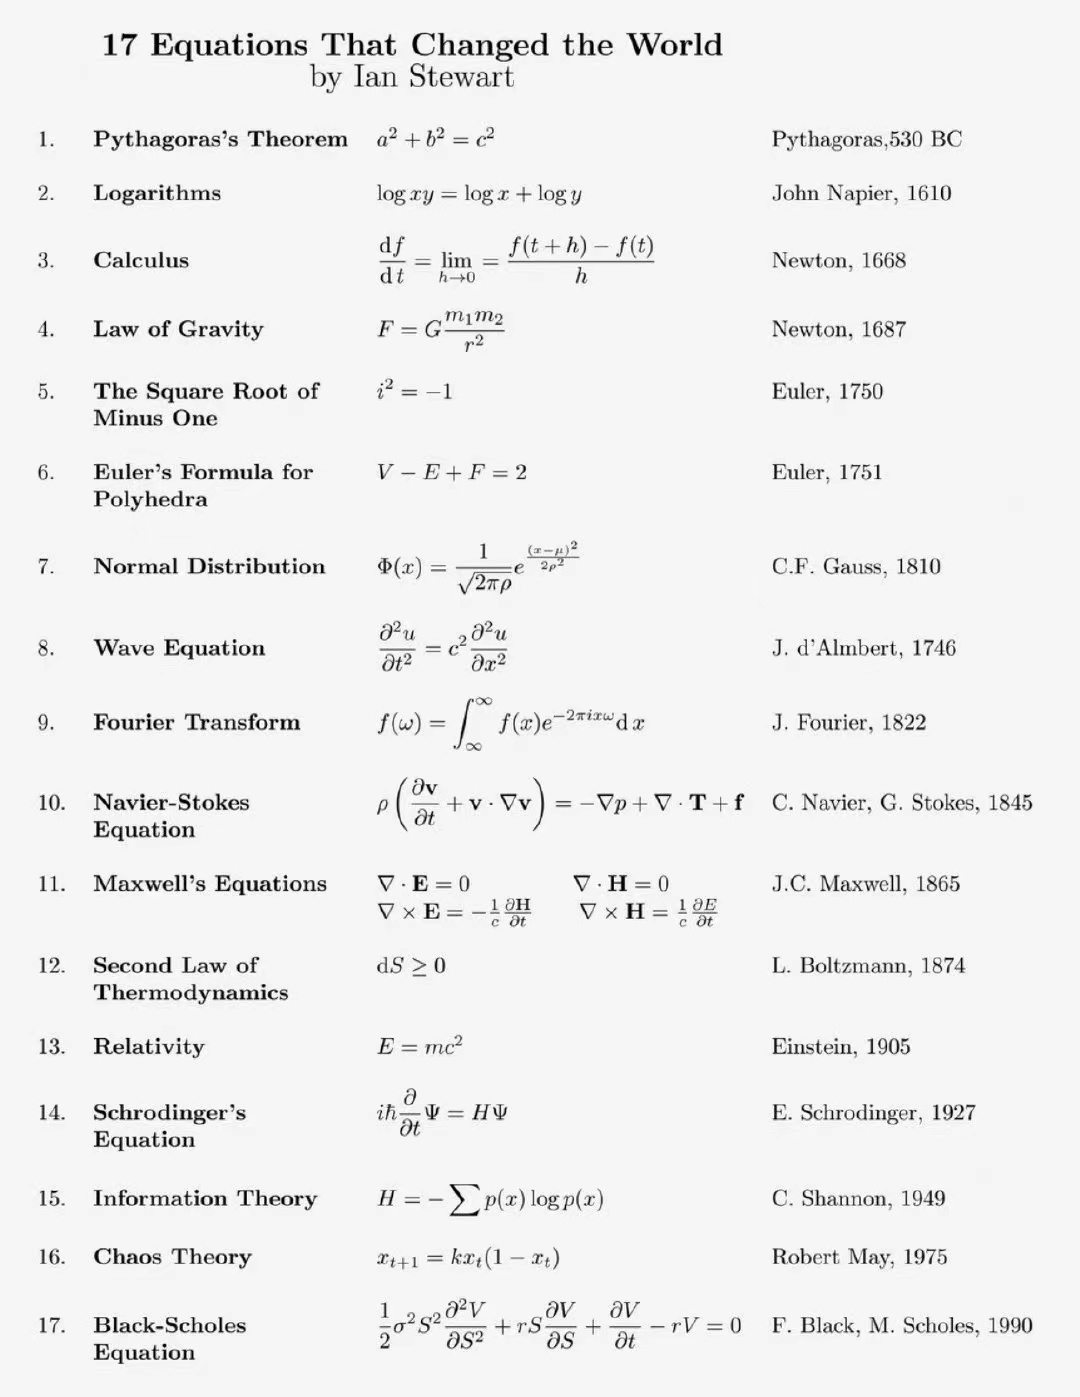
\includegraphics[height=2.85in,width=2.00in,viewport=0 0 780 1100,clip]{Figures/Great_Equation.jpg}
\label{Great_Equation}
\end{figure}
\end{minipage}
}

\frame
{
	\frametitle{量子力学的奠基人}
\begin{figure}[h!]
\centering
%\vspace{-25.5pt}
%\hspace*{-15.5pt}
%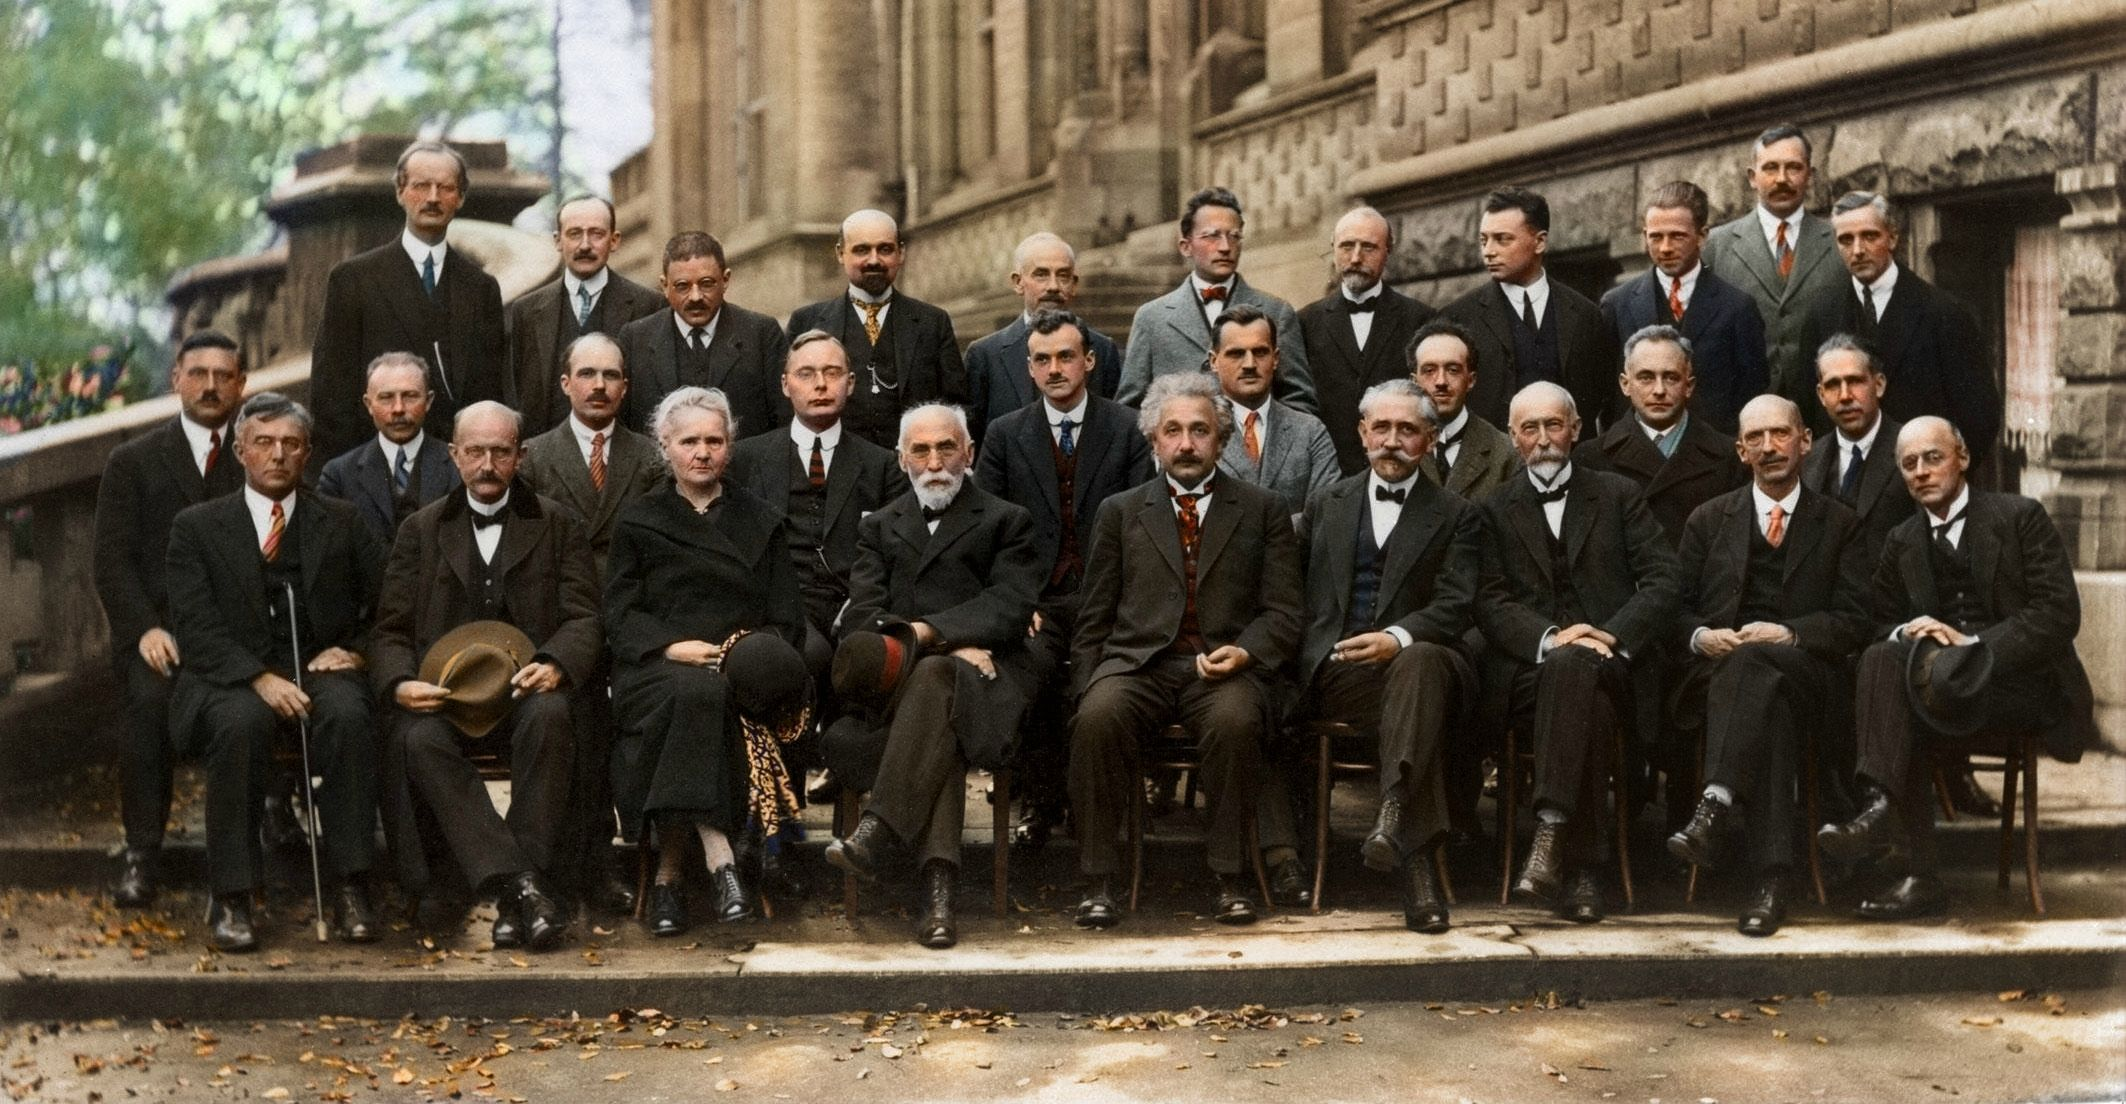
\includegraphics[height=0.57\textwidth,width=1.1\textwidth,viewport=0 0 2150 1050,clip]{Figures/Solvay_Conference-5-fine.jpg}
\vspace{-14.5pt}
\hspace*{-15.5pt}
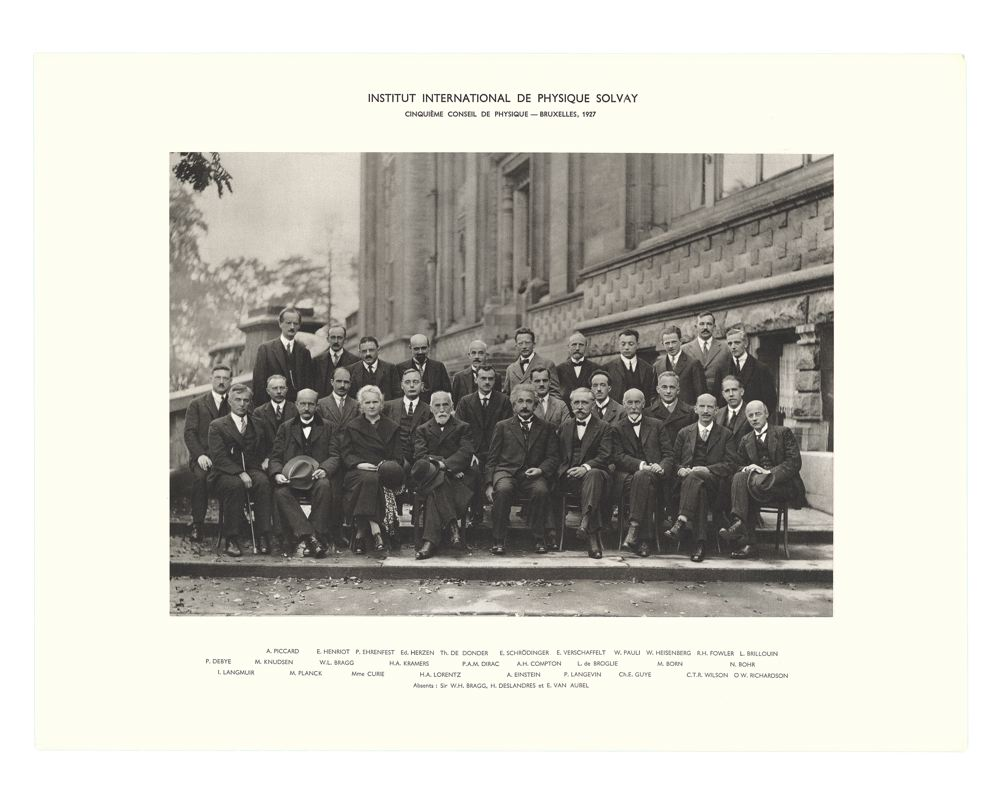
\includegraphics[height=0.50\textwidth,width=0.70\textwidth,viewport=150 105 850 710,clip]{Figures/Solvay_Conference-5.jpg}
\caption{\fontsize{7.5pt}{6.2pt}\selectfont{\textrm{The Fifth Solvay International Conference, Brussels, Belgium, Oct. 1927}}}
\label{Solvay Conference-5-fine}
\end{figure}
\vspace{-11.5pt}
\fontsize{4.1pt}{3.9pt}\selectfont{\textrm{\textcolor{blue}{前排左起}:~I.Langmuir(\textcolor{blue}{朗缪尔}) M.Planck(\textcolor{blue}{普朗克}) Marie Curie(\textcolor{blue}{居里夫人}) H.Lorentz(\textcolor{blue}{洛仑兹}) A.Einstein(\textcolor{blue}{爱因斯坦}) P.Langevin(\textcolor{blue}{朗之万}) Ch.E.Guye(\textcolor{blue}{古伊}) C.T.R.Wilson(\textcolor{blue}{威尔逊}) O.W.Richardson(\textcolor{blue}{理查森})\\
\textcolor{blue}{中排左起}:~P.Debye(\textcolor{blue}{德拜}) M.Knudsen(\textcolor{blue}{克努森}) W.L.Bragg(\textcolor{blue}{布拉格}) H.A.Kramers(\textcolor{blue}{克莱默}) P.A.M.Dirac(\textcolor{blue}{狄拉克}) A.H.Compton(\textcolor{blue}{康普顿}) L.de Broglie(\textcolor{blue}{德布罗意}) M.Born(\textcolor{blue}{玻恩}) N.Bohr(\textcolor{blue}{玻尔})\\
\textcolor{blue}{后排左起}:~A.Piccard(\textcolor{blue}{皮卡尔德}) E.Henriot(\textcolor{blue}{亨利厄特}) P.Ehrenfest(\textcolor{blue}{埃伦费斯特}) Ed.Herzen(\textcolor{blue}{赫尔岑}) Th.de Donder(\textcolor{blue}{德唐德}) E.Schr\"odinger(\textcolor{blue}{薛定谔}) E.Verschaffelt(\textcolor{blue}{费尔夏费尔特}) W.Pauli(\textcolor{blue}{泡利}) W.Heisenberg(\textcolor{blue}{海森堡}) R.H.Fowler(\textcolor{blue}{富勒}) L.Brillouin(\textcolor{blue}{布里渊})}}
}
%------------------------------------------------------------------------Reference----------------------------------------------------------------------------------------------
\frame
{
	\frametitle{态叠加原理:~\textrm{Schr\"odinger's cat}}
\begin{figure}[h!]
\centering
\vspace{-10.5pt}
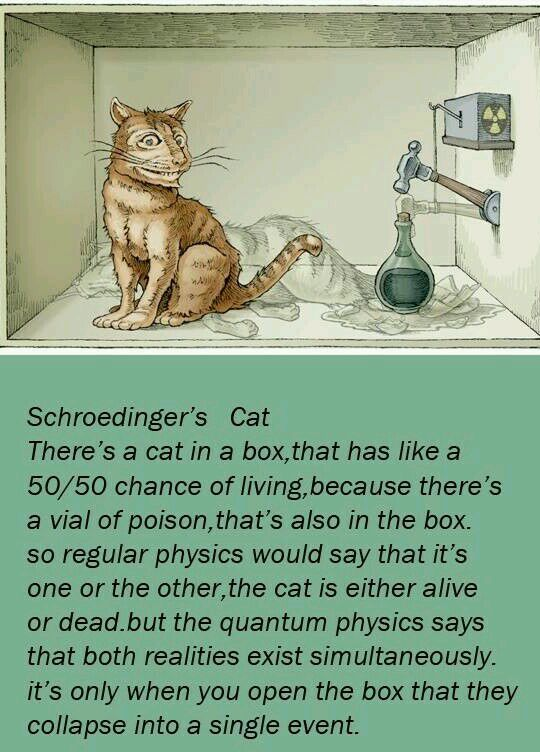
\includegraphics[height=0.70\textwidth,width=0.48\textwidth,viewport=0 0 550 750,clip]{Figures/Schrodinger-cat.jpg}
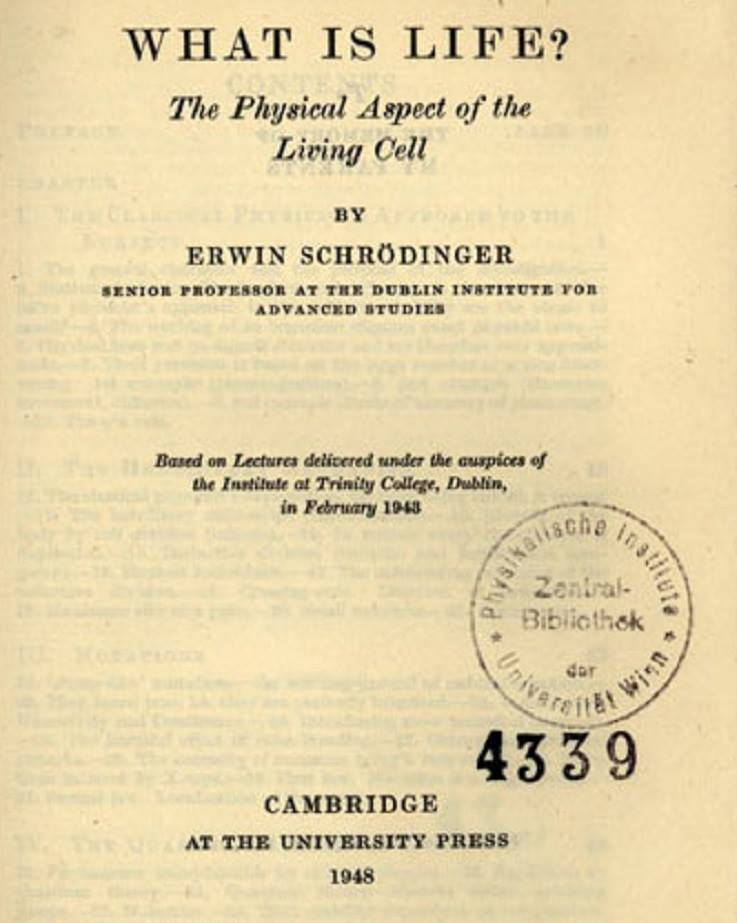
\includegraphics[height=0.70\textwidth,width=0.50\textwidth,viewport=0 0 720 930,clip]{Figures/Schrodinger_book.jpg}
%\caption{\textrm{ABINIT}的Si.in}
\label{Schrodinger-cat}
\end{figure}
}

\frame
{
	\frametitle{因果倒置:~\textrm{Delayed Choice Experiment}}
\begin{figure}[h!]
\centering
\vspace{-10.5pt}
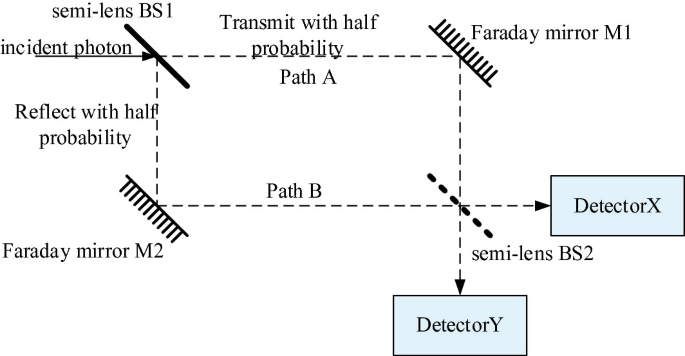
\includegraphics[height=0.55\textwidth,width=1.0\textwidth,viewport=0 0 690 370,clip]{Figures/Schematic-diagram-of-delayed_choice-experiment.png}
\caption{\fontsize{5.2pt}{3.9pt}\selectfont{\textrm{Schematic diagram of delayed choice experiment with A Mach-Zehnder Interferometer.}}}
\label{Delayed_Choice-Experiment}
\end{figure}
}

\frame
{
	\frametitle{量子力学量力学}
\begin{figure}[h!]
\centering
\vspace{-13.5pt}
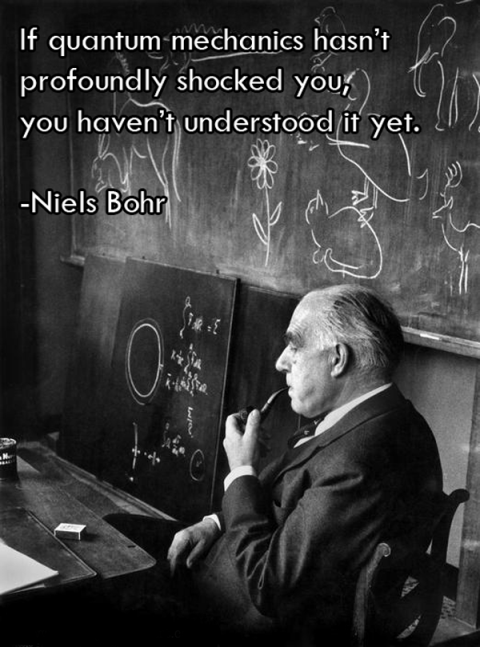
\includegraphics[height=0.75\textwidth,width=0.55\textwidth,viewport=0 0 500 650,clip]{Figures/Quote-Niels_Bohr-on-Quantum_mechanics.png}
\caption{\fontsize{5.2pt}{3.9pt}\selectfont{\textrm{A quote of Niels Bohr on Quantum mechanics.}}}
\label{Quote-Niels_Bohr}
\end{figure}
}

\frame
{
	\frametitle{几何原本:~公理体系的源头}
\begin{figure}[h!]
\centering
\vspace{-13pt}
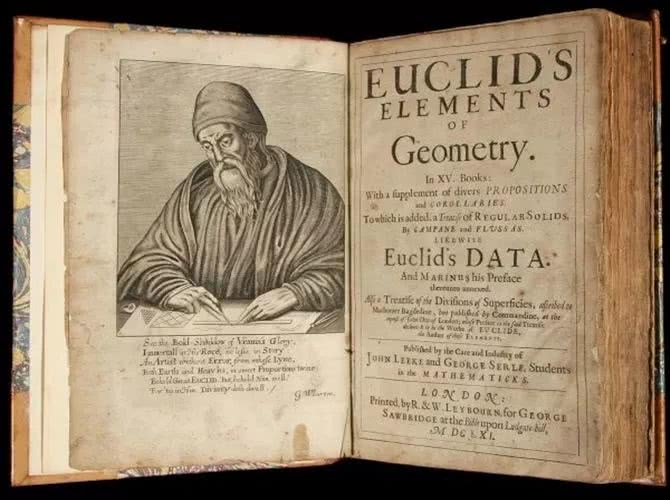
\includegraphics[height=0.38\textwidth,width=0.65\textwidth,viewport=0 0 680 500,clip]{Figures/Element_Geometry_1.jpg}\\
\vspace{1pt}
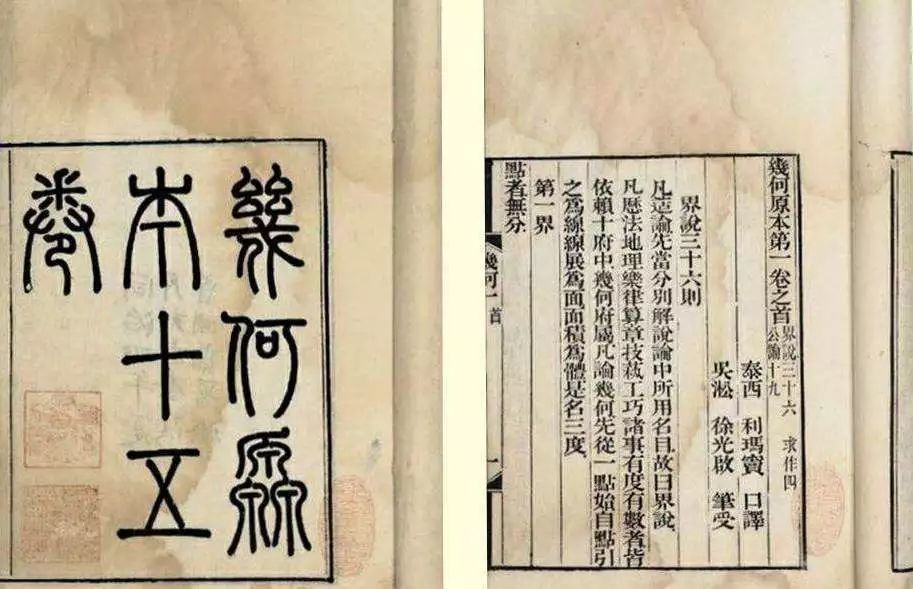
\includegraphics[height=0.36\textwidth,width=0.65\textwidth,viewport=0 0 810 500,clip]{Figures/Element_Geometry_2.jpg}
%\caption{\textrm{ABINIT}的Si.in}
\label{Element_Geometru}
\end{figure}
}

\frame
{
	\frametitle{\textcolor{red}{公理体系}:~现代科学的逻辑起点}
\begin{figure}[h!]
\centering
\vspace{-10.5pt}
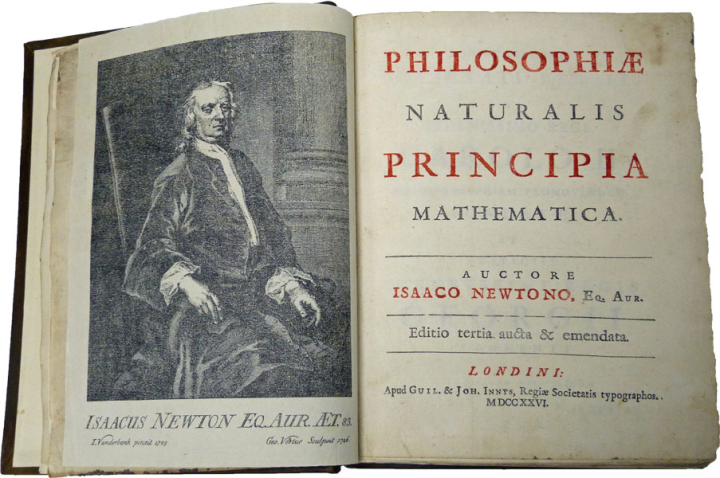
\includegraphics[height=0.68\textwidth,width=1.0\textwidth,viewport=0 0 770 500,clip]{Figures/Philp_Nature_Mach-2.png}
%\caption{\textrm{ABINIT}的Si.in}
\label{Philp_Nature}
\end{figure}
}

\frame[allowframebreaks]
{
	\frametitle{量子力学基本假设(\textcolor{red}{公理体系})}
	\begin{itemize}
		\item 全同粒子假设\\
			\textcolor{blue}{全同粒子组成的体系中,两个全同粒子相互调换不改变体系的状态}\\ 
			全同粒子是指\textcolor{red}{内禀性质完全相同的一类微观粒子}:\\例如,所有的电子是全同粒子 
		\item 波函数假设\\
			\textcolor{blue}{微观体系的运动状态可由波函数$\Psi$完全描述,波函数包含体系的所有性质}\\
			波函数$\Psi$一般要求满足\textcolor{red}{连续}、\textcolor{red}{有限}和\textcolor{red}{单值}三个条件
		\item 微观体系的运动状态\textcolor{blue}{波函数随时间变化的规律}:\\\textcolor{red}{遵从\textrm{Schr\"odinger}方程}
			$$\mathrm{i}\hbar\dfrac{\mathrm{d}}{\mathrm{d}t}|\Psi\rangle=\hat{\mathbf H}|\Psi\rangle$$
		\item 态叠加原理\\
			如果$\Psi_1$是体系的一个本征态,对应的本征值为$A_1$,$\Psi_2$也是体系的一个本征态,对应的本征值为$A_2$,则\textcolor{blue}{$$\Psi=C_1\Psi_1+C_2\Psi_2$$}\textcolor{red}{也是体系一个可能的存在状态}
		\item 力学量算符假设\\
			\textcolor{blue}{经典力学的物理量对应到量子力学中,要用线性~\textrm{Hermite}算符表示}(\textcolor{red}{\textrm{Hermite~}算符的本征函数构成完备空间})\\
			如动量算符 ~~~ $\hat{\mathbf{p}}=-\mathrm{i}\hbar\nabla$\\
			~~~位置算符 ~~~ $\hat{\mathbf r}=r$\\
			力学量算符之间有确定的对易关系(\textcolor{brown}{量子条件})
			$$[\hat{\mathbf F},\hat{\mathbf G}]=\hat{\mathbf F}\hat{\mathbf G}-\hat{\mathbf G}\hat{\mathbf F}$$ 
			
	\end{itemize}
}

\frame
{
	\frametitle{叠加态的数学表示:~矩阵}
\begin{figure}[h!]
\centering
\vspace{-1.5pt}
\hspace*{-0.12in}
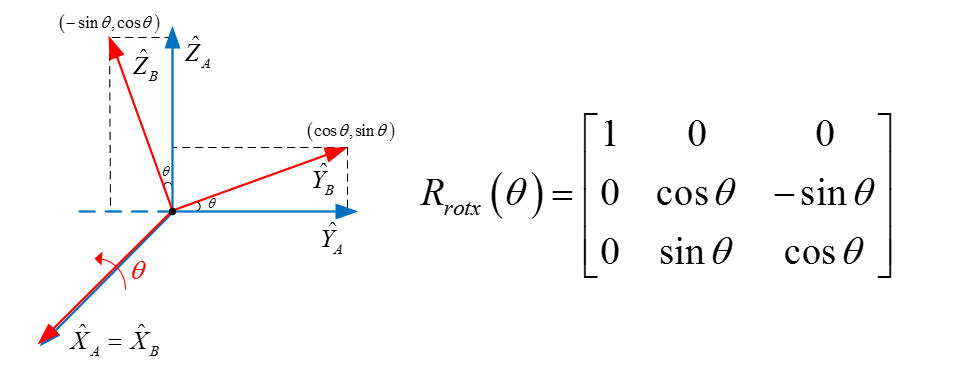
\includegraphics[height=0.48\textwidth,width=1.05\textwidth]{Figures/Matrix_Rotation.png}
%\caption{\textrm{ABINIT}的Si.in}
\label{Matrix-Rotation}
\end{figure}
}

\frame
{
	\frametitle{量子化学学科创立}
	\begin{itemize}
		\item \textrm{1927}年,\textrm{\o.~Burrau}应用量子力学原理,完成\textrm{\ch{H2+}}离子的计算
		\item 同年,\textrm{Walter~Heitlery}和\textrm{Fritz~W.~London}对\textrm{\ch{H2}}分子的计算,标志着量子化学这一学科正式创立
	\end{itemize}
\begin{figure}[h!]
\centering
\vspace{-1.5pt}
\hspace*{-0.12in}
\includegraphics[height=0.48\textwidth,width=0.80\textwidth,viewport=0 10 260 175,clip]{Figures/Walter-Heitlery_Fritz-W-London.jpeg}
\caption{\textrm{W.~Heitlery (left) and F.~W.~London(right).}}
\label{Heitlery_London}
\end{figure}
}

%\frame
%{
%	\frametitle{\textrm{Paul Adrian Maurice Dirac's Commandments}}
%	\textrm{The underlying laws necessary for the mathematical treatment of a large part of physics \textcolor{red}{and the whole of chemistry} are thus completely known, and the difficulty lies only in the fact that application of these laws leads to equations that are \underline{too complex to be solved}.
%\vskip 15pt
%It therefore becomes desirable that approximation practical methods of applying quantum mechanics should be develop $\cdots$ 
%}

%\vskip 15pt
%\textrm{P.A.M Dirac Proc. Roy. Soc. Ser. A, \textbf{123}, 714, (1929)}
%}
%
\frame
{
%	\frametitle{\rm{Paul Dirac's Commandments\upcite{PRSLSA123-714_1929}}}
	\frametitle{\textrm{Paul Dirac's Commandments}}%\upcite{PRSLSA123-714_1929}}}
%	\textrm{\textcolor{purple}{The underlying laws necessary for the mathematical treatment of a large part of physics and the whole of chemistry are thus completely known, and the difficulty lies only in the fact that application of these laws leads to equations that are too complex to be solved.}}
\begin{figure}[h!]
\centering
\vspace{-10.5pt}
\includegraphics[height=0.71\textwidth,width=0.9\textwidth,viewport=0 0 1150 920,clip]{Figures/Dirac_comment.png}
%\caption{\textrm{ABINIT}的Si.in}
\label{Diract_Commandment}
\end{figure}
}

%-----------------------------------------------------------------------------
\section{\rm{Hartree-Fock~}方法}
\frame
{
	\frametitle{\textrm{Born-Oppenheimer~}近似}
	\begin{itemize}
		\item 由于原子核的质量要比电子大很多(一般要大3-4个数量级),在同样的相互作用下,原子核的运动比电子也慢得多
		\item 电子在每一时刻仿佛运动在静止原子核构成的势场中,而原子核运动时则感受不到电子的具体位置,感受到的是运动电子的平均作用力
		\item 可近似将原子核坐标与电子坐标变量分离,使得求解整个体系的波函数的复杂过程分解为求解电子波函数和求解原子核波函数两个相对简单的过程\\
			电子运动方程$$\hat{\mathbf H}_{\mathrm e}(\vec r,\vec{\mathbf R})\Psi(\vec r,\vec{\mathbf R})=E_{\mathrm e}(\vec{\mathbf R})\Psi(\vec r,\vec{\mathbf R})$$
			原子核运动方程$$[\hat{\mathbf T}_{\mathrm{nul}}+E_{\mathrm e}(\vec{\mathbf R})]\chi(\vec{\mathbf R})=E\chi(\vec{\mathbf R})$$
	\end{itemize}
}

\frame
{
	\frametitle{独立粒子近似}
	\textrm{n-}粒子体系中的每个粒子的运动,完全忽略粒子间的瞬时相互作用,认为第$i$个粒子在其余$\mathrm{n}-1$个粒子组成的平均势场中运动
	$$\Psi(\vec r_1,\vec r_2,\vec r_3,\cdots,\vec r_n)=\psi_1(\vec r_1)\psi_2(\vec r_2)\psi_3(\vec r_3)\cdots\psi_n(\vec r_n)$$
	$$\hat{\mathbf H}=\sum_{i=1}^N-\dfrac{1}{2}\nabla_i^2+\sum_{i=1}^NV_i(\vec r_i)+\sum_{i,j(j\neq i)}\dfrac{e^2}{|\vec r_i-\vec r_j|}$$
	粒子$i$的\textrm{Hartree}算符
	$$\hat{\mathbf h}_i=-\dfrac{1}{2}\nabla_i^2+V_i(r_i)+\sum_{j(j\neq i)}^N\dfrac{e^2}{|\vec r_i-\vec r_j|}$$
	因此每个粒子的运动方程为:
	$$\hat{\mathbf h}_i\psi_i(\vec r)=\bigg[-\dfrac{1}{2}\nabla_i^2+V_i(r_i)+\sum_{j(j\neq i)}^N\dfrac{e^2}{|\vec r_i-\vec r_j|}\bigg]\psi_i(\vec r)=\varepsilon\psi_i(\vec r)$$ 
}

\frame
{
	\frametitle{\textrm{Slater~}行列式}
	简单乘积的独立粒子波函数不满足全同粒子置换对称性要求,不能正确表示电子不可辨认的物理属性
	
	\textrm{Slater}建议用行列式形式表示具有反对称性的波函数
	\begin{displaymath}
		\hspace*{-10pt}\Psi(\vec r_1,\vec r_2,\vec r_3,\cdots,\vec r_n)=\dfrac1{\sqrt{n!}}
		\left|\begin{array}{ccccc}
			\psi_1(\vec r_1)&\psi_2(\vec r_1)&\psi_3(\vec r_1)&\cdots&\psi_n(\vec r_1)\\
			\psi_1(\vec r_2)&\psi_2(\vec r_2)&\psi_3(\vec r_2)&\cdots&\psi_n(\vec r_2)\\
			\psi_1(\vec r_3)&\psi_2(\vec r_3)&\psi_3(\vec r_3)&\cdots&\psi_n(\vec r_3)\\
			&&&\cdots&\\
			\psi_1(\vec r_n)&\psi_2(\vec r_n)&\psi_3(\vec r_n)&\cdots&\psi_n(\vec r_n)
		\end{array}\right|
	\end{displaymath}
	粒子$i$的\textrm{Fock}算符
	$$\hat{\mathbf F}_i=-\dfrac{1}{2}\nabla_i^2+V_i(r_i)+\hat{\mathbf J}_i-\hat{\mathbf K}_i$$
	$$\hat{\mathbf J}_i(\vec r_i)=\int\dfrac{\psi_j^{\ast}(\vec r_j)|e^2|\psi_j(\vec r_j)}{|\vec r_i-\vec r_j|}\mathrm{d}\vec r_j$$
	$$\hat{\mathbf K}_i(\vec r_i)\psi_i(\vec r_i)=\psi_j(\vec r_i)\int\dfrac{\psi_j(\vec r_j)|e^2|\psi_i(\vec r_j)}{|\vec r_i-\vec r_j|}\mathrm{d}\vec r_j$$

}

\frame
{
	\frametitle{\textrm{Hartree-Fock-Roothan~}方法}
	实际求解非相对论的\textrm{Schr\"odinger}方程时,
	$$\hat{\mathbf F}_i\psi_i(\vec r_i)=\varepsilon_i\psi_i(\vec r_i)$$
	将波函数$\psi_i(\vec r_i)$用一套选定的基函数$\phi_j(\vec r)$展开
	$$\psi_i(\vec r)=\sum_{j=1}^Nc_{ij}\phi_j(\vec r)$$
	通过变分原理
	$$\bar E=\dfrac{\langle\Psi|\hat{\mathbf H}|\Psi\rangle}{\langle\Psi|\Psi\rangle}\geqslant E_0$$
	改变展开系数$c_{ij}$直到体系的能量最小,确定展开系数

	重复上述流程直至\textrm{Fock}算符$\hat{\mathbf F}$、波函数$\psi(\vec r)$和能量$\varepsilon$自洽,这就是\textrm{Hartree-Fock-Roothan}方法
}

\frame
{
	\frametitle{\textrm{RHF~}与\textrm{UHF}} 
	\begin{itemize}
		\item \textrm{RHF}:\\
			针对闭壳层(\textrm{closed shell})体系,占据轨道的电子成对出现,自旋相反,可用一个\textrm{Slater}行列式表示\\
	%		每对自旋相反的电子有相同的轨道波函数\\
			对于闭壳层体系,\textrm{Hartree-Fock}方法求解的能量本征值符合\textrm{Koopmans}定理
			$$E_{ion}^1=-\varepsilon_{\mathrm{HOMO}}$$
		\item \textrm{UHF}:\\
			针对开壳层(\textrm{open shell})体系,占据轨道有未成对电子,需要用\textrm{Slater}行列式的线性组合表示\\
			最低能态用一个\textrm{Slater}行列式,但不同自旋的轨道分别处理
		$$E_{\mathrm{UHF}}\leqslant E_{\mathrm{RHF}}$$
			由于\textrm{UHF}包含更多的变分函数,可以处理一些近解离极限的分子体系
	\end{itemize}
}

\frame
{
	\frametitle{\textrm{Slater~}的$\chi_{\alpha}$方法}
	由于\textrm{Hartree-Fock~}的交换势计算复杂,\textrm{Slater~}建议用电子密度的加权平均来简化交换势的求解
	\begin{displaymath}
		V_{\mathrm x}=-\frac{\sum\limits_i\sum\limits_jn_in_j\int\varphi_i^{\ast}(\vec r)\varphi_i(\vec r{}^{\prime})(2/|\vec r-\vec r{}^{\prime}|)\varphi_j^{\ast}(\vec r{}^{\prime})\varphi_j(\vec r)\mathrm{d}\vec r}{\sum\limits_kn_k\varphi_k^{\ast}(\vec r)\varphi_k(\vec r)}
	\end{displaymath}
	自由电子气在动量空间用\textrm{Hartree-Fock}方法表示
	\begin{displaymath}
		V_{\mathrm x}(k)=-8\left( \frac3{8\pi}\rho \right)^{1/3}F(\eta)
	\end{displaymath}
	这里$\eta=k/k_{\mathrm F}$,并有
	\begin{displaymath}
		F(\eta)=\frac12+\frac{1-\eta^2}{4\eta}\ln\left|\frac{1+\eta}{1-\eta}\right|
	\end{displaymath}
	$F(\eta)$在$\eta=1(k=k_{\mathrm F})$出现奇点(对应于自由电子气\textrm{Fermi~}面上电子密度为0)。
}
	
\frame
{
	\frametitle{\textrm{Slater~}的$\chi_{\alpha}$方法}
	\textrm{Slater~}建议,对占据态($k\leqslant k_{\mathrm F}$)的电子作加权平均,可有
	\begin{displaymath}
		F(\eta)=\frac{\int_0^1\eta^2F(\eta)\mathrm{d}\eta}{\int_0^1\eta^2\mathrm{d}\eta}=\frac34
	\end{displaymath}
	因此,对于均匀电子气,交换势
	\begin{displaymath}
		V_{\mathrm x}=-6\left( \frac3{8\pi}\rho \right)^{1/3}
	\end{displaymath}
	\textrm{Slater~}指出,对于局域电子密度$\rho(\vec r)$体系,可有\textrm{Slater~}交换势
	\begin{displaymath}
		V_{\mathrm xs}(\vec r)=-6\left( \frac3{8\pi}\rho(\vec r) \right)^{1/3}
	\end{displaymath}
	在此基础上,\textrm{Slater~}建议对上述交换势引入可调参数$\alpha$,有交换势
	\begin{displaymath}
		V_{\chi_{\alpha}}(\vec r)=\alpha V_{\mathrm xs}(\vec r)
	\end{displaymath}
}

\frame
{
	\frametitle{交换与相关}
	\begin{itemize}
		\item \textrm{Fock}算符中的交换算符$\hat{\mathrm K}_i(\vec r_i)$是由\textrm{Slater}行列式引入的,属于量子效应
	\end{itemize}
%	\vspace*{-5pt}
	\begin{displaymath}
%		\hspace*{-2pt}
		\text{电子间瞬时相互作用(\textcolor{red}{关联})}
		\left\{
			\begin{aligned}
				&\text{\textcolor{blue}{电子交换}:同自旋电子的关联作用}\\
				&\text{\textcolor{blue}{电子相关}}
			\end{aligned}
			\right.
	\end{displaymath}
\begin{figure}[h!]
\centering
\vspace{-10.5pt}
\includegraphics[height=0.42\textwidth,width=0.6\textwidth,viewport=0 0 760 550,clip]{Figures/Post-HF.png}
%\caption{\textrm{ABINIT}的Si.in}
\label{Post-HF}
\end{figure}
}

\frame
{
	\frametitle{\textrm{Post-HF}}
	\textrm{Hartree-Fock}方法精确定义了交换作用,完全没考虑电子相关作用
	\begin{itemize}
		\item \textrm{CI (Configuration Interaction)}
	$$\Psi=\sum_{I=0}C_I\Phi_I=C_0\Phi_0+C_1\Phi_1+C_2\Phi_2+\cdots$$
		\item \textrm{CC (Couple Cluste)}\\
			\begin{displaymath}
				\Psi=\mathrm{e}^{\hat{\mathbf T}}\Phi_0=\mathrm{e}^{(\hat{\mathbf T}_1+\hat{\mathbf T}_2+\hat{\mathbf T}_3+\cdots)}\Phi_0
			\end{displaymath}
		\item \textrm{MP}微扰方法
			\begin{displaymath}
				\begin{aligned}
					&\hat{\mathbf H}=\hat{\mathbf H}^{(0)}+\hat{\mathbf V} \\
					&\hat{\mathbf H}^{(0)}=\sum_i\hat{\mathbf F}_i \qquad \Phi^{(0)}=\Psi_{\mathrm{HF}}\\ 
					&\hat{\mathbf V}=\sum_{j>i}^{\mathrm occ}\dfrac{e^2}{r_{ij}}-\sum_{ij}^{\mathrm occ}\big(\hat{\mathbf J}_{ij}-\dfrac12\hat{\mathbf K}_{ij}\big)
				\end{aligned}
			\end{displaymath}
	\end{itemize}
}

\section{密度泛函理论}       %Bookmark
\subsection{\rm{Thomas-Fermi~}模型}       %Bookmark
\frame
{
	\frametitle{\textrm{Thomas-Fermi}模型} 
	1927年,\textrm{Thomas}和\textrm{Fermi}基于均匀电子气模型上建立\textrm{Thomas-Fermi}模型,\textcolor{blue}{体系能量可用}\textcolor{red}{电子密度}\textcolor{blue}{表示}:
	\begin{itemize}
		\item 动能表达式
			$$T_{\mathrm{TF}}[\rho(\vec r)]=\dfrac3{10}(3\pi^2)^{\frac23}\int\rho^{\frac53}(\vec r)\mathrm{d}\vec r$$
		\item 外势$V_{ext}(\vec r)$下电子体系的能量泛函表达式为
			\begin{displaymath}
				\begin{aligned}
					E_{\mathrm{TF}}[\rho(\vec r)]=&\dfrac3{10}(3\pi^2)^{\frac23}\int\rho^{\frac53}(\vec r)\mathrm{d}\vec r\\
					&+\int\rho(\vec r)V_{ext}(\vec r)\mathrm{d}\vec r+\dfrac12\int\int\dfrac{\rho(\vec r_1)\rho(\vec r_2)}{|\vec r_2-\vec r_1|}\mathrm{d}\vec r_1\mathrm{d}\vec r_2
				\end{aligned}
			\end{displaymath}
		\item \textrm{Thomas-Fermi}模型完全没有考虑电子的交换-相关作用
	\end{itemize}
}

\frame
{
	\frametitle{\textrm{Thomas-Fermi-Dirac}模型} 
	1930年,\textrm{Dirac}将\textrm{Thomas-Fermi}模型修正,用局域密度近似考虑电子交换作用
			\begin{displaymath}
				\begin{aligned}
					E_{\mathrm{TFD}}[\rho(\vec r)]=&\dfrac3{10}(3\pi^2)^{\frac23}\int\rho^{\frac53}(\vec r)\mathrm{d}\vec r+\int\rho(\vec r)V_{ext}(\vec r)\mathrm{d}\vec r\\
					&+\dfrac12\int\int\dfrac{\rho(\vec r_1)\rho(\vec r_2)}{|\vec r_2-\vec r_1|}\mathrm{d}\vec r_1\mathrm{d}\vec r_2-\dfrac34\bigg(\dfrac3{\pi}\bigg)^{\frac13}\int\rho^{\frac43}(\vec r)\mathrm{d}\vec r
				\end{aligned}
			\end{displaymath}
			\begin{itemize}
				\item 在总电子数守恒约束条件
					$$\int\rho(\vec r)\mathrm{d}\vec r=N$$
					下,能量泛函$E_{\mathrm{TFD}}[\rho(\vec r)]$对密度$\rho(\vec r)$的变分极小获得体系的基态密度和基态能量
			\end{itemize}
}

\frame
{
	\frametitle{\textrm{Thomas-Fermi}模型}
	\begin{itemize}
		\item \textrm{Thomas-Fermi}模型用电子密度代替波函数描述问题是极大的简化,但模型过于粗糙:\\
%			\begin{enumerate}
%				\item 以均匀电子气的密度得到动能的表达式
%				\item 完全忽略电子间的交换-相关作用
%			\end{enumerate}
			不能正确描述相互作用电子体系的基本特征,如原子的壳层结构
		\item \textrm{Thomas-Fermi}模型虽不够精确,但可以通过引入修正项校正:
			\textrm{Dirac}交换泛函 $$E_X[\rho(\vec r)]=-\dfrac34\bigg(\dfrac3{\pi}\bigg)^{\frac13}\int\rho^{\frac43}(\vec r)\mathrm{d}\vec r$$
			\textrm{Wigner}相关泛函 $$E_C[\rho(\vec r)]=-0.056\int\dfrac{\rho^{\frac43}(\vec r)}{0.079+\rho^{\frac13}(\vec r)}\mathrm{d}\vec r$$
	\end{itemize}
	\textrm{Thomas-Fermi}模型为密度泛函理论\textrm{(DFT)}提供了重要的启示
}

\subsection{密度泛函理论}       %Bookmark
\frame                               %
{
\frametitle{密度泛函理论(\textrm{DFT})} %Slide Page Title
%   \secname
与传统的量子力学方法不同,密度泛函理论的基本变量是体系的基态电子密度。%通过体系的电子密度而非波函数确定体系的基态能量。
\begin{itemize}%[+-| alert@+>]
	\item 密度泛函理论的基石:\textrm{Hohenberg-Kohn}定理\upcite{PR136-B864_1964}
\vskip 5pt
\begin{itemize}%[+-| alert@+>]
   \setlength{\itemsep}{8pt}
 \item $E[\rho]=F_{\mathrm{HK}}[\rho]+\displaystyle\int\rho(\vec{r})v(\vec{r})\textrm{d}\vec{r}$ \\
\vskip 5pt 其中$F_{\mathrm{HK}}[\rho]=\underset{\Psi\to\rho}{\mathrm{Min}}\langle\Psi[\rho]|\hat{T}+\hat{W}|\Psi[\rho]\rangle$
是普适的泛函表达式。%,指明多电子体系的基态性质与基态密度间存在一一对应关系
     \textrm{\small{第一定理表明多电子体系的性质完全由体系的基态密度决定}}
   \item 如果$\tilde\Psi\neq\Psi$,
     $E[\tilde\rho]\geqslant E[\rho_0]$\\
     \textrm{\small{第二定理指出基态总能量泛函在体系基态电子密度处取极小值}}
   \end{itemize}
%\textrm{\small{第二定理指出基态总能量泛函在体系基态电子密度处取极小值}}
\vskip 8pt
 \item 密度泛函理论的优越性:用密度($\rho$)代替波函数($\Psi$)描述体系
\vskip 5pt
 \item 密度泛函理论的困难:能量密度泛函的精确形式未知
   \end{itemize}
}

\frame
{
	\frametitle{\rm{Creators of DFT}}
\begin{figure}[h!]
\vskip 10pt
\centering
\includegraphics[height=1.65in,width=4.0in,viewport=0 0 1562 610,clip]{Figures/Creators_of_DFT.png}
\caption{\tiny \textrm{Creators of DFT. Walter Kohn(left, in 1962) and his two postdoctoral fellows, Pierre Hohenberg (middle, in 1965) and Lujeu Sham (right).}}%(与文献\cite{EPJB33-47_2003}图1对比)
\label{Creator_of_DFT}
\end{figure}
}

\frame                               %
{
\frametitle{密度泛函理论(\textrm{DFT})}
\textrm{Kohn-Sham}方程\upcite{PR140-A1133_1965}:无相互作用体系+交换-相关能的贡献
$$(T_S+V_{e\!f\!f})|\varphi_i\rangle=\varepsilon_i|\varphi_i\rangle,\quad i=1,\cdots,N,\cdots$$
其中$T_S=-\dfrac12\nabla^2$~~是无相互作用体系的动能
\begin{displaymath}
	\begin{aligned}
		V_{e\!f\!f}(\vec r)=&V_{ext}(\vec r)+\displaystyle\int w(\vec r,\vec r\,')\rho(\vec r\,')\mathrm{d}\vec r\,'+V_{\mathrm{XC}}[\rho]\\
=&\displaystyle\int\dfrac{\rho(\vec r\,')}{|\vec r-\vec r^{\prime}|}\mathrm{d}\vec r\,'+V_{ext}(\vec r)+V_{\mathrm{XC}}[\rho]
	\end{aligned}
\end{displaymath}
$V_{ext}(\vec r)$是电子体系与外部的电荷或磁场相互作用\\
$V_{\mathrm{XC}}[\rho]=\dfrac{\delta E_{\mathrm{XC}}}{\delta\rho(\vec r)}$称为交换-相关势
\vskip 10pt
\textrm{Kohn-Sham}方程是形式上的单粒子方程
\vskip 6pt
\textrm{Kohn-Sham}方程的实质:\\\textcolor{red}{将动能泛函的主要部分分离出来,剩余部分放在交换-相关能中}
}

\frame
{
\frametitle{交换-相关能与交换-相关势}
实际考虑交换-相关能时,会将交换-相关能表示为交换能和相关能之和:
\begin{displaymath}
	E_{\mathrm{XC}}[\rho]=E_{\mathrm{X}}[\rho]+E_{\mathrm{C}}[\rho]=\int\varepsilon_{\mathrm{X}}[\rho]\rho(\vec{r}) \textrm{d}^3\vec{r}+\int\varepsilon_{\mathrm{C}}[\rho]\rho(\vec{r}) \textrm{d}^3\vec{r}
\end{displaymath}
$\varepsilon_{\mathrm{X}}[\rho]$和$\varepsilon_{\mathrm{C}}[\rho]$可理解为单电子的交换能和相关能
\vskip 20pt
交换-相关势通过交换-相关能计算得到:~
		\begin{displaymath}
			V_{\mathrm{XC}}^{\sigma}[\rho_{\alpha},\rho_{\beta}]=\dfrac{\delta E_{\mathrm{XC}}[\rho_{\alpha},\rho_{\beta}]}{\delta\rho_{\sigma}}=\dfrac{\delta\{E_{\mathrm{X}}[\rho_{\alpha},\rho_{\beta}]+E_{\mathrm{C}}[\rho_{\alpha},\rho_{\beta}]\}}{\delta\rho_{\sigma}}
		\end{displaymath}
		\textcolor{red}{注意}:~由于$E_{\mathrm{XC}}[\rho_{\sigma}]$对$\rho_{\sigma}$是非线性的\\
		\textcolor{blue}{$V_{\mathrm{XC}}=V_{\mathrm{X}}+V_{\mathrm{C}}$和$\varepsilon_{\mathrm{XC}}=\varepsilon_{\mathrm{X}}+\varepsilon_{\mathrm{C}}$不同,不要混淆这两个量}
}
%  \beamertemplateshadingbackground{blue!10}{yellow!10}

\frame                               %
{
\frametitle{交换-相关能密度泛函}
\textcolor{blue}{密度泛函理论的核心问题}:\\
\textrm{Kohn-Sham}方程用于实际计算,必须知道$E_{XC}[\rho]$或者$V_{XC}[\rho]$与$\rho(\vec r)$的泛函关系
\vskip 15pt
\begin{minipage}[b]{0.59\textwidth}
 \hspace*{-15pt}
 {\fontsize{7.5pt}{6.0pt}\selectfont\begin{itemize}%[+-| alert@+>]
	 \setlength{\itemsep}{10pt}
 \item \textrm{LDA}:泛函只与密度分布的局域值有关
 \item \textrm{GGA}:泛函依赖:局域密度及其梯度
 \item $meta$-\textrm{GGA}:泛函依赖的变量还有动能密度
 \item 杂化(\textrm{hybrid})泛函:泛函与占据轨道有关
 \item 其他的交换-相关能泛函
 \item<1-> 完全非局域泛函:理想泛函,不现实
 \end{itemize}}
\end{minipage}
\hfill
\begin{minipage}[b]{0.39\textwidth}
\hspace*{-10pt}
\includegraphics[height=1.7in,width=3.18in,viewport=10 5 1380 700,clip]{Figures/Jacobi-ladder.png}\\
\centering{\textcolor{red}{\textrm{\tiny Jacob's ladder}}}
\end{minipage}
% \begin{itemize}%[+-| alert@+>]
%\item 交换-相关能密度泛函
}

\frame                               %
{
	\frametitle{近似能量泛函$E_{\mathrm{XC}}[\rho]$的主要问题}
\vskip 20pt
\begin{enumerate}%[+-| alert@+>]
   \setlength{\itemsep}{10pt}
 \item  密度是整体变量:~电子自相互作用抵消不净\\%\quad\textrm{(LDA+U)}方法的校正%(\textrm{LDA+U})
	 用\textrm{DFT}计算电子数很少的体系,一般都会有较大的误差
 \item  电子相关:~简并和近简并基态的表示不合理\\
	 基态电子密度用不同的简并轨道计算时,体系能量应保持不变,但现有的近似能量泛函不具有这个性质
 \item  渐近行为:~处理弱相互作用体系的误差大\\
	 如\textrm{Van der Waals}相互作用和现有近似能量泛函本身的计算误差在同一量级
 \end{enumerate}
}

\frame
{
	\frametitle{\textrm{DFT-SCF}}
\begin{figure}[h!]
\centering
\vspace*{-0.25in}
\hspace*{-0.80in}
\includegraphics[height=2.80in,width=4.95in,viewport=5 3 1490 870,clip]{Figures/DFT-SCF_2.png}
%\caption{\tiny \textrm{Pseudopotential for metallic sodium, based on the empty core model and screened by the Thomas-Fermi dielectric function.}}%(与文献\cite{EPJB33-47_2003}图1对比)
\label{DFT-SCF-2}
\end{figure}
}

\frame
{
	\frametitle{\textit{ab~initio}和\textrm{first~principle}}
	\begin{itemize}
		\item \textit{ab~initio}是拉丁文词汇\textrm{(Latin~term)},其含义是\textrm{``from the beginning''},由拉丁文\textit{ab}~\textrm{(``from'')}+\textit{initio}~\textrm{(``beginning'')}合成,后者是\textit{initium}的单数夺格\footnote{\fontsize{5.5pt}{4.2pt}\selectfont{夺格\textrm{(ablative)},又称离格或从格,语法功能上表示某些词汇的状语。拉丁文\textit{initium}的意思是''开始、初始''。}}
		\item \textit{ab~initio}常用于法律和科学领域,如从头计算法(\textit{ab~initio}~\textrm{method})。法律中,\textit{ab~initio}表示"一开始即如此,而非法院宣判之后"。
		\item \textrm{first~principle}指从基本的物理学定律出发,不外加假设与经验拟合的推导与计算。
		\item 在物理学领域,\textrm{first~principle}(第一性原理)和\textit{ab~initio}(从头计算)含义上是等价的。例如利用\textrm{Schr\"odinger}方程在一些近似条件下求解电子结构,但无须依赖实验数据得到拟合参数的方法,就是第一原理或从头计算法。
	\end{itemize}
}

\frame
{
	\frametitle{\textit{ab~initio} \textrm{in inscription}}
\begin{figure}[h!]
\vspace*{-0.15in}
\centering
\includegraphics[height=2.10in,width=1.55in,viewport=5 3 1550 2180,clip]{Figures/Madonna-Ss.-Dominic-and-Thomas_Aquinas-3.jpeg}
\hspace*{15pt}
\includegraphics[height=2.10in,width=1.15in,viewport=5 3 950 1880,clip]{Figures/Madonna-Ss.-Dominic-and-Thomas_Aquinas-Inscription_2.jpeg}
%\caption{\tiny \textrm{Pseudopotential for metallic sodium, based on the empty core model and screened by the Thomas-Fermi dielectric function.}}%(与文献\cite{EPJB33-47_2003}图1对比)
\label{ABINITIO-inscription}
\end{figure}
\begin{minipage}{0.53\textwidth}
	{\fontsize{8.2pt}{4.2pt}\selectfont{ 
		\centering{MEMOR}\\
		\centering{ESTO}\\
		\centering{CONGREGATIONIS}\\
		\centering{TV\AE}\\
		\centering{QVAM}\\
		\centering{POSSEDISTI}\\
		\centering{\textcolor{red}{ABINITO}\\}}}
\end{minipage}
\hspace*{5pt}
\begin{minipage}{0.30\textwidth}
	\textrm{\fontsize{4.2pt}{4.2pt}\selectfont{The inscription in English:}}\\
	\textrm{\fontsize{8.2pt}{4.2pt}\selectfont{\textcolor{blue}{Mind the congregation that has been yours} \textcolor{purple}{since the beginning}}}
\end{minipage}
}

%-----------------------------------------------------------------------------
\section{固体能带理论}       %Bookmark
\frame
{
%\frametitle{The Bloch theorem}
	\frametitle{\textrm{Bloch~}定理}
\begin{itemize}%[+-| alert@+>]
   \setlength{\itemsep}{8pt}
   \item 固体能带理论\upcite{Huang-Han}是固体电子理论的基础,形式上是单电子理论:
    $$\hat H |\psi_i^{\vec k}(\vec r)\rangle=\bigg[-\dfrac{\hbar^2}{2m}\nabla^2+V(\vec r)\bigg]|\psi_i^{\vec k}(\vec r)\rangle=\epsilon_i(\vec k)|\psi_i^{\vec k}(\vec r)\rangle$$
  \item \textrm{Bloch}定理:
%   \item \textrm{periodic potential:} $$V(\vec r)=V(\vec r+\vec R_n)$$
%     \textrm{Here,} $\vec R_n=n\vec R$
%   \item \textrm{Bloch theorem:}$$\psi_{\vec k}(\vec r)=\textrm{e}^{\textrm i\vec k\cdot\vec r}u_{\vec k}(\vec r)$$
%     \textrm{Here, $u_{\vec k}(\vec r)$ is a periodic function with the same periodicity as $V(\vec r)$, i.e., $u_{\vec k}(\vec r)=u_{\vec k}(\vec r+\vec R_n)$, then Bloch theorem could reads as:}
%     $$\psi_{\vec k}(\vec r+\vec R_n)=\textrm{e}^{\textrm i\vec k\cdot\vec R_n}\psi_{\vec k}(\vec r)$$
具有平移周期性的理想晶体,势能$V(\vec r)$满足$$V(\vec r)=V(\vec r+\vec R_n)$$
体系的波函数满足\textrm{Bloch}波函数形式:$$\psi_{\vec k}(\vec r)=\textrm{e}^{i\vec k\cdot\vec r}u_{\vec k}(\vec r)$$
是平面波和周期函数的乘积。$u(\vec r)$与势能有相同的周期。即$$u_{\vec k}(\vec r)=u_{\vec k}(\vec r+\vec R_n)$$
  \item 能带理论相当于分子轨道理论
%   \setlength{\itemsep}{30pt}
\item \textrm{Bloch}函数反映了波函数在周期性势场下的变化规律。
\end{itemize}
}

\frame
{
\frametitle{周期体系的波函数}
物质的电子体系,可分为芯层分子和价层电子。芯电子能量低,受周围化学环境影响很小,基本保持原子属性;价层电子相互作用较强,对化学环境较为敏感。一般地,价电子波函数在原子间区域(\textrm{Interstitial}区)的变化平缓,在临近原子核附近区域(\textrm{Muffin-tin}球内),会出现剧烈振荡(与芯层波函数正交)。
\begin{figure}[h!]
\centering
\includegraphics[height=0.8in,width=4.in,viewport=41 433 539 546,clip]{Figures/Pseudo_wave.pdf}\\
\includegraphics[height=0.8in,width=4.in,viewport=41 210 539 339,clip]{Figures/Pseudo_wave.pdf}
\caption{\tiny \textrm{The periodic Potential and the wave functions in crystal.}}%(与文献\cite{EPJB33-47_2003}图1对比)
\label{Potential-Wave}
\end{figure}
}

\frame
{
\frametitle{一维自由电子近似微扰}
\begin{figure}[h!]
\centering
%\hspace*{-10pt}
%\vspace*{-1.1in}
\includegraphics[height=1.5in,width=2.5in,viewport=5 5 700 450,clip]{Figures/Band_Gap-2.png}
%\caption{\tiny \textrm{The Band-structure from free-electron gas.}}%
\label{Band-Gap-2}
\end{figure} 
\begin{displaymath}
	\begin{aligned}
		&\hat H_0=-\dfrac{\hbar^2}{2m}\dfrac{\mathrm{d}^2}{\mathrm{d}x^2}+\={V} \longrightarrow \hat H=\hat H_0+\hat H^{\prime}=-\dfrac{\hbar^2}{2m}\dfrac{\mathrm{d}^2}{\mathrm{d}x^2}+\={V}+\underline{V(x)-\={V}}\\
		&\Psi_k^0(x)=\dfrac1{\sqrt V}\mathrm{e}^{\mathrm{i}k\cdot x} \longrightarrow \Psi_k(x)=\Psi_k^0(x)+\sum_{k^{\prime}\neq k}\dfrac{\langle k^{\prime}|\hat H^{\prime}|k\rangle}{E_k^0-E_{k^{\prime}}^0}\Psi_{k^{\prime}}^0(x)\\
		&\hat E_k^0=-\dfrac{\hbar^2k^2}{2m}+\={V} \longrightarrow E_k=%E_k^0+E^{\prime}=
		\dfrac{\hbar^2k^2}{2m}+\={V}+\sum_n{}^{\prime}\dfrac{|V_n|^2}{\frac{\hbar^2}{2m}[k^2-(k+2\pi\frac na)^2]}
	\end{aligned}
\end{displaymath}
}

\frame
{
\frametitle{一维自由电子简并微扰}
在波矢$k=\pm\frac{n\pi}{a}$位置,电子能量出现简并态,必须采用简并态微扰理论处理
\begin{figure}[h!]
\centering
%\hspace*{-10pt}
%\vspace*{-1.1in}
\includegraphics[height=1.3in,width=1.4in,viewport=0 5 420 450,clip]{Figures/Band_Gap-1.png}
%\caption{\tiny \textrm{The Band-structure from free-electron gas.}}%
\label{Band-Gap-1}
\end{figure} 
\begin{displaymath}
	E_{\textcolor{red}{\pm}}=\left\{
	\begin{aligned}
		&T_n+\={V}\textcolor{red}{+}\Delta^2T_n\bigg(\dfrac{2T_n}{|V_n|}\textcolor{red}{+}1\bigg)\\
		&T_n+\={V}\textcolor{red}{-}\Delta^2T_n\bigg(\dfrac{2T_n}{|V_n|}\textcolor{red}{-}1\bigg)
	\end{aligned}\right.
\end{displaymath}
这里$T_n=\frac{\hbar^2}{2m}\big(\frac{n\pi}a\big)^2$
}

\frame
{
\frametitle{自由电子气模型}
简并态微扰理论引起的能带裂分
\begin{figure}[h!]
\centering
%\hspace*{-10pt}
%\vspace*{-1.1in}
\includegraphics[height=2.1in,width=3.8in,viewport=10 90 570 380,clip]{Figures/Band_Gap.pdf}
\caption{\tiny \textrm{The Band-structure from free-electron gas.}}%
\label{Band-Gap-co}
\end{figure} 
}

\frame
{
\frametitle{紧束缚模型}
从分子轨道到能带
\begin{figure}[h!]
\centering
\hspace*{-0.29in}
\vspace*{-0.1in}
\subfigure[一维$\mathrm{H}$原子链]{
\label{fig:Hydrogen-1D}
\includegraphics[height=0.25in,width=1.1in,viewport=70 255 570 375,clip]{Figures/Hydrogen-1D.pdf}}
\subfigure[$\mathrm{H}_n$分子轨道]{
\label{fig:Hydrogen-2-n}
\includegraphics[height=0.8in,width=1.5in,viewport=30 140 545 480,clip]{Figures/Hydrogen-Mol-Orbital.pdf}}
\subfigure[分子波函数]{
\label{fig:Hydrogen-Psi}
\includegraphics[height=0.5in,width=1.4in,viewport=25 218 595 440,clip]{Figures/Hydrogen-Psi.pdf}}\\
\vspace*{5pt}
\subfigure[分子轨道与能带]{
\label{fig:Hydrogen-Band-1D}
\includegraphics[height=0.6in,width=1.4in,viewport=35 215 575 450,clip]{Figures/Hydrogen-Band-1D.pdf}}
\subfigure[$d$\,轨道]{
\label{fig:Hydrogen-d-Band-1D}
\includegraphics[height=1.0in,width=0.7in,viewport=40 45 330 535,clip]{Figures/Hydrogen-d-Band-1D.pdf}}
\caption{\tiny \textrm{The Band-structure from Molecular-orbital.}}%
\label{Band-Structure-local-orbit}
\end{figure} 
}

\subsection{能带、$\vec k$-空间与~\rm{Fermi~}面}
\frame
{
\frametitle{能带、$\vec k$空间与\textrm{Fermi}面}
\vspace{30pt}
\begin{figure}[h!]
\centering
\hspace*{-0.10in}
\subfigure[\textrm{Band structure}]{
\label{Band_Gap_Fermi-1}
\includegraphics[height=1.6in,width=2.1in,viewport=0 0 480 350,clip]{Figures/Band_Brillouin_zone.png}}
\subfigure[\textrm{Brillouin Zone}]{
\label{Band_Gap_Fermi-2}
\includegraphics[height=1.28in,width=1.75in,viewport=100 120 545 470,clip]{Figures/2D_Brillouin-Zone.pdf}}
\label{Band_Gap_Fermi}
\end{figure}
}

\frame
{
	\frametitle{简单立方体系的\textrm{Brillouin}区与能带}
\vspace{10pt}
\begin{figure}[h!]
\centering
\hspace*{-0.28in}
\subfigure[\textrm{Brillouin Zone of Cubic lattice}]{
\label{Brillouin_Zone_Cubic-1}
\includegraphics[height=2.1in,width=2.0in,viewport=90 0 550 500,clip]{Figures/Brillouin-Zone_CUB.png}}
\subfigure[\textrm{Band Structure of \ch{SrSnO3}}]{
\label{Band_Gap_SrSnO3-1}
\vspace*{-1.00in}
\includegraphics[height=2.10in,width=1.75in,viewport=0 0 710 550,clip]{Figures/Band-Struct_SrSnO3.png}}
\label{Band_Gap_CUB_SrSnO3}
\end{figure}
}

\frame
{
	\frametitle{面心立方体系的\textrm{Brillouin}区与能带}
\vspace{10pt}
\begin{figure}[h!]
\centering
\hspace*{-0.30in}
\subfigure[\textrm{Brillouin Zone of FCC lattice}]{
\label{Brillouin_Zone_FCC}
\includegraphics[height=1.9in,width=1.8in,viewport=75 0 560 520,clip]{Figures/Brillouin-Zone_FCC.png}}
\subfigure[\textrm{Band structure of \ch{CdS}}]{
\label{Band_Gap_CdS}
\includegraphics[height=2.10in,width=1.95in,viewport=0 0 700 520,clip]{Figures/Band-Struct_CdS.png}}
\label{Band_Gap_FCC_CdS}
\end{figure}
}

\frame
{
	\frametitle{体心立方体系的\textrm{Brillouin}区与能带}
\vspace{10pt}
\begin{figure}[h!]
\centering
\hspace*{-0.30in}
\subfigure[\textrm{Brillouin Zone of BCC lattice}]{
\label{Brillouin_Zone_BCC}
\includegraphics[height=2.1in,width=1.9in,viewport=80 0 550 520,clip]{Figures/Brillouin-Zone_BCC.png}}
\subfigure[\textrm{Band structure of \ch{GeF4}}]{
\label{Band_Gap_GeF4}
\includegraphics[height=2.10in,width=1.95in,viewport=0 0 700 500,clip]{Figures/Band-Struct_GeF4.png}}
\label{Band_Gap_BCC_GeF4}
\end{figure}
}

\subsection{固体能带计算方法}
\frame
{
%\frametitle{The methods on band structure calculation}
\frametitle{固体能带计算方法}
%\vskip 10pt
%\textrm{The mainly difference of all these methods below: the basis sets and the construction of the potential}
\vskip 10pt
常用的计算方法
\begin{itemize}%[+-| alert@+>]
%\begin{enumerate}%[+-| alert@+>]
\setlength{\itemsep}{12pt}
%  \item \textrm{Plane wave and the pseudo-potential}
	\item	平面波方法
	\item	正交平面波\textrm{(The orthogonalized plane wave, OPW)}和赝势\textrm{(Pseudo-potential, PP)}方法\upcite{Singh,PRB41-7892_1990,JPCM6-8245_1994}
	\item	缀加平面波\textrm{(Augmented plane wave, APW)}方法
	\item	\textrm{MT}轨道\textrm{(Muffin-tin orbitals, MTO)}方法
	\item	投影子缀加波\textrm{(Projector Augmented Wave, PAW)}方法\upcite{PRB50-17953_1994,PRB59-1758_1999}
\end{itemize}
\vskip 5pt 各种方法的\textcolor{red}{主要区别}:~\textcolor{blue}{势函数的处理}与\textcolor{blue}{所选基函数类型}不同
}

\frame                               %
{
	\frametitle{\textrm{Kohn-Sham}方程}
\begin{figure}[h!]
\centering
\vspace*{-0.21in}
\hspace*{-0.1in}
\includegraphics[height=2.7in,width=4.0in,viewport=2 5 1162 880,clip]{Figures/DFT.png}
\caption{\tiny \textrm{The Analysis of Kohn-Sham equation.}}%(与文献\cite{EPJB33-47_2003}图1对比)
\label{DFT}
\end{figure}
}

\frame
{
\frametitle{电荷密度的重新分解}
%\textrm{PAW}方法提出后有很长一段时间没有能够得到广泛应用,直到\textrm{G. Kresse}等将\textrm{Bl\"ochl}的原始方案中电荷密度计算方案重新组合后,明确了\textrm{PAW}方法与\textrm{USPP}方法的内在联系。
\begin{itemize}
	\item 芯层电荷与核电荷构成离子实电荷:$n_{Zc}=n_Z+n_c$
\end{itemize}
\begin{figure}[h!]
\centering
\vspace{-10.5pt}
\includegraphics[height=1.8in,width=4.0in,viewport=0 0 380 190,clip]{Figures/Pseudo-potential_charge.png}
%\caption{\tiny \textrm{The difference of the electron-density distributing from P.~Bl\"ochl  and from G.~Kresse.}}%(与文献\cite{EPJB33-47_2003}图1对比)
\label{PAW_Pseudo-Charge}
\end{figure}
}

\frame
{
	\frametitle{球形势对平面波的散射}
\begin{figure}[h!]
\centering
\vspace*{-0.26in}
\includegraphics[height=1.90in,width=2.48in,viewport=0 0 400 300,clip]{Figures/Pseudo-scatter.jpg}
\caption{\fontsize{5.5pt}{4.2pt}\selectfont{\textrm{Schematic illustration of scattering of a plane wave by a spherical potential.}}}%(与文献\cite{EPJB33-47_2003}图1对比)
\label{Pseudo-scatter}
\end{figure}
\vspace*{-0.1in}
\fontsize{7.5pt}{6.2pt}\selectfont{
入射平面波
$$\mathrm{e}^{\mathrm{i}\vec q\cdot\vec r}=4\pi\sum_{lm}\mathrm{i}^lj_l(\vec q\cdot\vec r)Y_{lm}^{\ast}(\hat{\vec q})Y_{lm}(\hat{\vec r})=\sum_{l}(2l+1)\mathrm{i}^lj_l(qr)P_{l}(\cos\theta)$$
%$$\mathrm{e}^{\mathrm{i}\vec q\cdot\vec r}=\mathrm{e}^{\mathrm{i}qr\cos(\theta)}=\sum_{l}(2l+1)\mathrm{i}^lj_l(qr)P_{l}[\cos(\theta)]$$
}
}

\frame
{
	\frametitle{势阱与相移}
\begin{figure}[h!]
\centering
\vspace*{-0.26in}
\includegraphics[height=1.85in,width=1.3in,viewport=0 0 750 1050,clip]{Figures/Radial_wave_functions_for_various_square_well_potential.png}
\caption{\fontsize{5.5pt}{4.2pt}\selectfont{\textrm{The radial wave functions for \textit{l}=0 for various square well potential depths.}}}%(与文献\cite{EPJB33-47_2003}图1对比)
\label{Pseudo-scatter}
\end{figure}
\vspace*{-0.1in}
\fontsize{7.5pt}{6.2pt}\selectfont{
平面波经散射后出射,波函数变为
$$\Psi_l^{>}(\varepsilon,r)=C_l\bigg[j_l(\kappa r)-\tan\eta_l(\varepsilon)n_l(\kappa r)\bigg]\quad\text{其中}\kappa^2=\varepsilon$$
根据散射理论,能量为$\varepsilon$的电子经单个势阱散射偏转$\theta$后,波函数的振幅可以表示为
	\begin{displaymath}
		t(\theta)=\dfrac{4\pi}{\kappa}\sum_l(2l+1)[\mathrm{exp}(2\mathrm{i}\eta_l(\varepsilon))-1]P_l(\cos\theta)
	\end{displaymath}
%$$t(\theta)=\dfrac{4\pi}{\sqrt\varepsilon}\sum_l(2l+1)\bigg[\mathrm{e}^{2\mathrm{i}\eta_l(\varepsilon)}-1\bigg]P_l(\cos\theta)$$
%$$\eta_l(\varepsilon)=p_l\pi+\delta_l(\varepsilon)$$
}
}

\frame
{
	\frametitle{球形势散射的相移与赝势}
\begin{figure}[h!]
\centering
\vspace*{-0.20in}
\includegraphics[height=1.20in,width=1.77in,viewport=0 0 1150 750,clip]{Figures/Pseudo-scatter-2.png}
\caption{\fontsize{4.5pt}{3.2pt}\selectfont{\textrm{Radial wave-function $\phi=r\psi$ for low-energy scattering as illustrated in a figure from the 1934 and 1935 papers of Fermi and coworkers for low-energy electron scattering from atoms and neutron scattering from nuclei. The node in the wave-function near the origin show that the potential is attractive and strong enough to have bound states. The cross-section for scattering from the localized potential is determined by the phase shift and is the same for weaker pseudo-potential with the same phase shift modulo $2\pi$.}}}%(与文献\cite{EPJB33-47_2003}图1对比)
\label{Pseudo-scatter-2}
\end{figure}
\fontsize{7.5pt}{6.2pt}\selectfont{
对于球形势散射,相移可由径向波函数计算
$$\tan\eta_l(\varepsilon)=\dfrac{R\frac{\mathrm{d}}{\mathrm{d}r}j_l(\kappa r)|_R-D_l(\varepsilon)j_l(\kappa R)}{R\frac{\mathrm{d}}{\mathrm{d}r}n_l(\kappa r)|_R-D_l(\varepsilon)n_l(\kappa R)}$$
$$\mbox{其中~}D_l(\varepsilon,r)\equiv r\psi_l^{\prime}(r)/\psi_l(r)=r\dfrac{\mathrm{d}}{\mathrm{d}r}\ln\psi_l(r)$$
同时相移与波函数节点的关系为:$$\eta_l(\varepsilon)=p_l\pi+\delta(\varepsilon)$$}
}

%\frame
%{
%\begin{figure}[h!]
%\centering
%\vskip -3pt
%\includegraphics[height=2.5in,width=1.7in,viewport=0 0 600 850,clip]{Figures/Ouyang_Xiu-2.jpg}
%\hskip 20pt
%\includegraphics[height=2.5in,width=1.7in,viewport=0 0 600 790,clip]{Figures/Sale_Oil_Ouyang.png}
%\label{Sale_Oil_Ouyang}
%\caption{\tiny \textrm{欧阳修的《归田录\!$\cdot$\!卖油翁》.}}%(与文献\cite{EPJB33-47_2003}图1对比)
%\end{figure}
%}
%

\frame
{
%	\frametitle{\textrm{DFT-SCF}}
\begin{figure}[h!]
\vspace*{-0.25in}
\centering
\includegraphics[height=2.80in,width=4.95in,viewport=5 3 1250 780,clip]{Figures/Method_Procedure.png}
%\caption{\tiny \textrm{Pseudopotential for metallic sodium, based on the empty core model and screened by the Thomas-Fermi dielectric function.}}%(与文献\cite{EPJB33-47_2003}图1对比)
\label{Method-Procedure}
\end{figure}
}

%-----------------------------------------------------------------------------------------------------------------------------------------------------------------------%
\section{\rm{PAW}方法}
\frame
{
%	\frametitle{\textrm{PAW}原子数据集}
	\frametitle{\textrm{PAW Augmentation}}
\begin{figure}[h!]
\centering
\includegraphics[height=2.3in,width=4.0in,viewport=0 0 1280 745,clip]{Figures/PAW-baseset.png}
\caption{\tiny \textrm{The Augmentation of PAW.}}%(与文献\cite{EPJB33-47_2003}图1对比)
\label{PAW_baseset}
\end{figure}
}

\section{\rm{VASP}软件}
\frame
{
	\frametitle{\textrm{VASP}软件简介}
	\textrm{VASP}软件是维也纳大学\textrm{(Universit\"at Wien)}~\textrm{G. Kresse}等开发的第一原理模拟软件包
	\begin{itemize}
		\item \textrm{VASP}采用\textrm{PAW~(Projector Augmented-Wave)}方法\upcite{PRB50-17953_1994,PRB59-1758_1999},平衡了赝势方法和全电子计算优点,兼顾了计算的精度和效率
		\item \textrm{VASP}在实空间优化投影函数\textrm{(Projector)},将主要的计算过程变换到实空间完成,大大节省了内存的开销%,保证了计算精度和效率
		\item \textrm{VASP}通过引入多样的优化算法,提高了矩阵对角化和电荷密度搜索的效率
		\item 在\textrm{VASP}的并行计算中,有效均衡了各节点处理\textrm{FFT}变换负载和通信,提升了软件的并行效率
	\end{itemize}
	相比于其他第一原理计算软件,\textrm{VASP}从物理思想与方法、优化算法和并行计算实现等多个方面都有更为出色的性能
}

\frame
{
	\frametitle{\textrm{VASP}的开发团队}
\begin{figure}[h!]
\centering
\vspace*{-0.25in}
\includegraphics[height=2.70in,width=4.05in,viewport=330 130 1280 770,clip]{Figures/VASP_team.png}
\caption{\tiny \textrm{The development team of VASP.}}%(与文献\cite{EPJB33-47_2003}图1对比)
\label{VASP_team}
\end{figure}
}

\frame
{
	\frametitle{\textrm{VASP}的\textrm{Kohn-Sham}方程求解流程}
\begin{figure}[h!]
	\vspace{-0.2in}
\centering
%\includegraphics[height=2.7in,width=4.0in,viewport=0 0 1300 960,clip]{Figures/VASP_procedure-full.png}
%\includegraphics[height=2.1in,width=1.6in,viewport=0 0 480 630,clip]{Figures/VASP_procedure.png}
%\includegraphics[height=2.1in,width=2.3in,viewport=0 0 740 600,clip]{Figures/Ab-initio-Ene.png}
\includegraphics[height=2.75in,width=2.5in,viewport=0 0 480 630,clip]{Figures/VASP_procedure.png}
\caption{\tiny \textrm{The Flow of calculation for the KS-ground states.}}%(与文献\cite{EPJB33-47_2003}图1对比)
\label{PAW_baiseset}
\end{figure} 
}

\frame
{
	\frametitle{\textrm{VASP}的优化与迭代收敛}
	\textrm{VASP}计算中,资源消耗的主要部分是求解\textrm{Kohn-Sham}方程,即偏微分方程\textrm{(Partial Differential Equations,~PDE)}的自洽迭代, 迭代过程主要包括
	\begin{itemize}
		\item 矩阵的迭代对角化
		\item 电荷密度的自洽迭代
	\end{itemize}

	\vskip 10pt
	\textrm{VASP}的计算高效得益于求解过程中中应用了多种经典优化算法,保证了迭代计算的快速收敛
	\begin{itemize} 
		\item 拟牛顿法\textrm{(Quasi-Newton method)}
		\item 共轭梯度法\textrm{(Conjugate Gradients method, CG)}
		\item 残差最小化\textrm{(RMM-DIIS)}方法
	\end{itemize}
}

\frame
{
	\frametitle{\textrm{VASP}的并行效率}
	与同类型软件相比,\textrm{VASP}有着优异的并行能力
\begin{figure}[h!]
	\vspace{-0.15in}
\centering
%\includegraphics[height=2.7in,width=4.0in,viewport=0 0 1180 875,clip]{Figures/dual_grid.png}
\includegraphics[height=1.55in,width=1.95in,viewport=0 0 240 200,clip]{Figures/VASP-abinit_Li128-1.png}
\includegraphics[height=1.55in,width=1.95in,viewport=0 0 240 200,clip]{Figures/VASP-abinit_Li128-2.png}
\caption{\tiny \textrm{The comparison of parallel scaling for ABINIT vs VASP.}}%(与文献\cite{EPJB33-47_2003}图1对比)
\label{ABINIT_vs_VASP}
\end{figure} 
\begin{itemize}
	\item \textrm{VASP}迭代对角化约束了矩阵的维度,减少了对角化过程中的迭代次数,保证了\textrm{MPI}并行的规模和扩展性
	\item \textrm{VASP}实施\textrm{FFT}变换时,保证各节点上处理的网格负载均衡
\end{itemize}
}

%\frame[allowframebreaks]
\begin{frame}[allowframebreaks]{\textrm{VASP}的主程序结构}
\begin{figure}[h!]
\vskip -10pt
\centering
\includegraphics[height=2.65in,width=4.0in,viewport=0 360 562 720,clip]{Figures/VASP_main_Flow-1.png}
\includegraphics[height=2.65in,width=4.0in,viewport=0 0 562 360,clip]{Figures/VASP_main_Flow-1.png}
\includegraphics[height=2.35in,width=4.0in,viewport=0 370 562 680,clip]{Figures/VASP_main_Flow-2.png}
\includegraphics[height=2.50in,width=4.0in,viewport=0 0 562 370,clip]{Figures/VASP_main_Flow-2.png}
\includegraphics[height=2.45in,width=4.0in,viewport=0 350 562 660,clip]{Figures/VASP_main_Flow-3.png}
\includegraphics[height=2.50in,width=4.0in,viewport=0 0 562 350,clip]{Figures/VASP_main_Flow-3.png}
\includegraphics[height=2.30in,width=4.0in,viewport=0 215 562 530,clip]{Figures/VASP_main_Flow-4.png}
\includegraphics[height=1.40in,width=4.0in,viewport=0 0 562 215,clip]{Figures/VASP_main_Flow-4.png}
\caption{\tiny \textrm{The Flow of main program for VASP.}}%(与文献\cite{EPJB33-47_2003}图1对比)
\label{FLOW_of_VASP}
\end{figure}
\end{frame}

\subsection{小结}
\frame
{
	\frametitle{小结}
	作为第一性原理计算的商用软件,\textrm{VASP}已成为计算材料学领域应用最广泛的软件之一。全球绝大多数超算中心都安装了\textrm{VASP},据统计,\textrm{VASP}软件的作业机时占用全球总机时的12$\sim$20\%,但由于其%类似于linpack软件,
属于重型浮点计算密集型应用,实际耗电量占比则高达30$\sim$50\%
\vskip 3pt
	{\fontsize{9.0pt}{7.2pt}\selectfont{
	\begin{itemize}
		\item \textcolor{blue}{物理上},\textrm{VASP}基于\textrm{DFT}近似,求解\textrm{Kohn-Sham}方程,并将粒子基态密度问题转化为矩阵的本征函数和本征值问题
		\item \textcolor{blue}{数学上},方程求解过程的核心是矩阵对角化与\textrm{PDE}的自洽迭代,即便对于简单体系,也需要完成数十次的迭代,而规模大的计算模拟体系则可能需要成千上万次迭代计算
		\item \textcolor{blue}{计算过程上},\textrm{VASP}计算的时长开销主要是本征值求解的矩阵对角化;此外由于算法限制,\textrm{Kohn-Sham}方程作为线性方程组作并行处理时,节点间存在密集的通信。在上千节点,上万计算核的大规模并行系统上,数据通信将严重影响程序的性能,这是当前\textrm{VASP}软件的主要瓶颈
	\end{itemize}}}
			\textcolor{magenta}{有必要探索新的并行和优化策略来提升\textrm{VASP}的计算性能}
}

%-----------------------------------------------------------------------------------------------------------------------------------------------------------------------%
\section{$\vec k$~空间布点与积分}
\frame
{
	\frametitle{$\vec k$~空间布点与\textrm{Fermi~}面的确定}
\begin{figure}[h!]
\centering
\hspace*{-0.35in}
\subfigure[\textrm{Brillouin Zone of Cubic lattice}]{
\label{Brillouin_Zone_Cubic-2}
\vspace*{-0.50in}
\includegraphics[height=2.10in,width=2.00in,viewport=90 0 550 500,clip]{Figures/Brillouin-Zone_CUB.png}}
\subfigure[\textrm{Band Structure of SrSnO$_3$}]{
\label{Band_Gap_SrSnO3-2}
\vspace*{-0.50in}
\includegraphics[height=2.10in,width=1.95in,viewport=0 0 710 550,clip]{Figures/Band-Struct_SrSnO3.png}}
\label{Band_Gap_CUB_SrSnO3}
\end{figure}
在固体能带理论中,能量色散关系$\varepsilon(\vec k)$~表示能量在倒空间中分布,其中量子数$\vec k$~(晶体动量)描述平移对称性
%\textcolor{blue}{能带图表示能量在\textrm{Brillouin-zone~}特定方向的色散关系}
}

\frame
{
	\frametitle{$\vec k$~空间布点与\textrm{Fermi~}面的确定}
\begin{figure}[h!]
\centering
%\hspace*{-10pt}
\vspace*{-0.3in}
\includegraphics[height=1.5in,width=4.1in,viewport=0 5 1400 500,clip]{Figures/Brillouin-Band.png}
\caption{\tiny \textrm{The relation between unfolded-Band and the Brillouin-zone.}}%
\label{Brillouin-Band}
\end{figure} 
周期体系的\textrm{Fermi~}能级和\textrm{Fermi~}面的确定:\\
\begin{displaymath}
	\left\{
	\begin{aligned}
		&\mbox{\textcolor{red}{导体:~}}&\mbox{\textcolor{blue}{价电子在\textrm{Brillouin-zone~}部分填充}}\\
		&\mbox{\textcolor{red}{半导体-绝缘体:~}}&\mbox{\textcolor{blue}{价电子在\textrm{Brillouin-zone~}完全填充}}
	\end{aligned}\right.
\end{displaymath}
}

\frame
{
	\frametitle{$\vec k$~空间布点与\textrm{Fermi~}面的确定}
\begin{figure}[h!]
\centering
%\hspace*{-10pt}
\vspace*{-0.3in}
\includegraphics[height=1.2in,width=1.3in,viewport=0 0 110 100,clip]{Figures/FS-Li.jpg}
\includegraphics[height=1.2in,width=1.3in,viewport=0 0 110 100,clip]{Figures/FS-Mg.jpg}
\includegraphics[height=1.2in,width=1.3in,viewport=0 0 110 100,clip]{Figures/FS-Cu.jpg}
\caption{\tiny \textrm{The Fermi-surface of Li, Mg, Cu in the first Brillouin-zone.}}%
\label{Brillouin-Band-Fermi}
\end{figure} 
\textcolor{blue}{\textrm{Fermi~}面的形状}:\\
\textcolor{red}{最高占据能带折叠到第一\textrm{Brillouin-zone~}围成的区域}

\vspace{10pt}
要确定\textrm{Fermi~}面的精细结构,\underline{\textcolor{red}{特别是对于金属和导体体系}},必须在整个\textrm{Brillouin-zone~}取足够多的采样点
}

\frame
{
\frametitle{$\vec k$~空间积分与物理量计算}
与\textrm{Fermi~}面的确定类似,周期体系中所有单粒子期望值可表示为整个\textrm{Brillouin-zone~}内占据态的矩阵元的积分\\

一般地,如果已知\textrm{Brillouin-zone~}某点$\vec k$~的能带指标为$n$的波函数本征态$\Psi_n(\vec k)$~和本征值$\epsilon_n(\vec k)$,算符$\mathbf{X}$~的期望值$\langle X \rangle$是矩阵元
\begin{displaymath}
	X_n(\vec k)=\langle\Psi_n(\vec k)|\mathbf{X}|\Psi_n(\vec k)\rangle 
\end{displaymath}
\textcolor{blue}{在倒空间全部占据能带的求和}
\begin{displaymath}
	\langle X\rangle=\dfrac1{\sqrt V_G}\sum_n\int_{V_G}\mathrm{d}^3kX_n(\vec k)f(\varepsilon_n(\vec k))
\end{displaymath}
其中$V_G$是第一\textrm{Brillouin-zone}体积,$f(\varepsilon)$~是占据分布函数

实际计算中,\textrm{Brillouin-zone~}的$\vec k$~点数是有限的
\begin{displaymath}
	\langle X\rangle=\sum_{j,n}X_n(\vec k_j)w_n^{\vec k_j}
\end{displaymath} 
\textcolor{blue}{$\vec k$~点数目决定了电子结构和物理量的的精度与计算量}
}

\frame
{
\frametitle{$\vec k$~空间布点方案}
\begin{enumerate}
	\item \textcolor{red}{简单分布函数}\\
		\begin{itemize}
			\item 
				\begin{figure}[h!]
					\begin{minipage}[t]{0.40\linewidth}
						\textrm{Fermi-Dirac~}分布函数$$f(\varepsilon)=\dfrac1{\mathrm{e}^{(\varepsilon-\mu)/kT}+1}$$ 
						其中$\mu$是化学势,$k$~是\textrm{Boltzmann}常数,$T$是温度参数
					\end{minipage}
				\hfill
					\begin{minipage}[t]{0.55\linewidth}
					\centering
					\vspace*{-0.35in}
					\hspace*{-0.5in}
					\includegraphics[height=1.0in,width=1.25in,viewport=0 0 530 500,clip]{Figures/Fermi-Dirac-distribution.jpg}
					\caption{\textrm{The Fermi-Dirac Distribution.}}%
					\label{Fermi-Dirac-distribution}
					\end{minipage}
					%\hspace*{-10pt}
				\end{figure} 
			\item 
				\begin{figure}[h!]
					\begin{minipage}[t]{0.40\linewidth}
						\textrm{Gaussian~}分布函数$$f(\varepsilon)=\dfrac1{\sigma\sqrt{2\pi}}\mathrm{e}^{-\frac{(\varepsilon-\mu)^2}{2\sigma^2}}$$
						其中$\mu$是化学势,$\sigma$是展宽参数
					\end{minipage}
				\hfill
					\begin{minipage}[t]{0.55\linewidth}
					\centering
					\vspace*{-0.35in}
					\hspace*{-0.5in}
					\includegraphics[height=1.0in,width=1.25in,viewport=0 0 530 500,clip]{Figures/Gaussian-distribution.jpg}
					\caption{\tiny \textrm{The Gaussian Distribution.}}%
					\label{Gaussian-distribution}
					\end{minipage}
					%\hspace*{-10pt}
				\end{figure} 
%			\item \textrm{Lorentz~}分布函数$$L(x)=\frac1{\pi}\frac{\frac12\Gamma}{(x-x_0)^2+\left(\frac12\Gamma\right)^2}$$
%				这里$x_0$是中心,$\Gamma$是展宽参数
		\end{itemize}
\end{enumerate}
}

\frame
{
\frametitle{$\vec k$~空间布点方案}
\begin{enumerate}
	\setcounter{enumi}{1}
\setlength{\itemsep}{10pt}
	\item \textcolor{red}{特殊点方法\textrm{(Special-point scheme)}}\\这是一种相对高效的积分方法,通过选取少量有代表性的$\vec k$~点,即可获得较高的计算精度,这些$\vec k$~点被称为“平均值点”或“特殊点”\\特殊点方法对导体的收敛性较差
	\item \textcolor{red}{四面体方法\textrm{(Tetrahedron schemen)}}\\这是一种线性插值方法,将\textrm{Brillouin-zone~}用体积相等的四面体填充,在每个四面体内部,被积函数$X_n(\vec k_j)$和能量$\varepsilon_n^{\vec k_j}$都随$\vec k$~点线性变化\\一般来说,四面体方法对金属和导体的\textrm{Fermi~}面确定更可靠
\end{enumerate}
\textcolor{blue}{如何方便地确定每个$\vec k$~点的积分权重$w_n^{\vec k_i}$,精确、高效地完成\textrm{Brillouin-zone~}积分是$\vec k$~空间布点方案的主要研究内容}
}

\frame
{
	\frametitle{各种$\vec k$~空间积分方法的比较}
\vskip -7pt
\begin{footnotesize}
\arrayrulewidth=0.4pt
\doublerulesep=0.4pt
\begin{table}[!h]
\tabcolsep 0pt \vspace*{-12pt}
%\begin{minipage}{\textwidth}
\label{tab:magno-1}
\centering
\def\temptablewidth{1.01\textwidth}
{\rule{\temptablewidth}{0.8pt}}
\begin{tabular*} {\temptablewidth}{|c@{\extracolsep{\fill}}|c|c|c|c|}
	\multirow{3}{*}{\textcolor{red}{积分方案}}	&\multicolumn{4}{c|}{\textcolor{blue}{布点方案}:~\textrm{Monkhorst-Pack}~方法} \\\cline{2-5}
	&\multirow{2}{*}{\textrm{Fermi-Dirac}~方法} &\multicolumn{2}{c|}{\textrm{Methfessel-Paxton}~方法} &\multirow{2}{*}{\textrm{Tetrahedron}~方法}\\\cline{3-4}
& &\textrm{Gaussian~} &$N>0$ & \\ \hline
半导体、&\multirow{2}{*}{\textcolor{blue}{$\texttimes$}} &$\delta\leqslant0.05$ &\multirow{2}{*}{\textcolor{red}{$\texttimes$}} &\textcolor{blue}{\textrm{DOS \& total-Energy}}\\
绝缘体 & &\textcolor{blue}{$\checkmark$} & &\textcolor{red}{$\checkmark$} \\\hline
导体、 & \multirow{2}{*}{\textcolor{blue}{$\checkmark$}} & \multicolumn{2}{c|}{\textcolor{blue}{\textrm{Phonon \& relaxation}}} &\textcolor{blue}{\textrm{DOS \& total-Energy}} \\
金属 & &\multicolumn{2}{c|}{\textcolor{red}{$\checkmark$}}  &\textcolor{red}{$\checkmark$} \\\hline
\multirow{2}{*}{\textrm{supercell}} &\multirow{2}{*}{\textcolor{blue}{$\checkmark$}} &\multicolumn{2}{c|}{\multirow{2}{*}{\textcolor{red}{$\checkmark$}}} &\multirow{2}{*}{\textcolor{red}{$\texttimes$}}\\
& &\multicolumn{2}{c|}{} &\\
\end{tabular*}
{\rule{\temptablewidth}{1pt}}\\
%\end{center}1
%\end{minipage}
\end{table}
\end{footnotesize}
}
%\frame
%{
%\begin{figure}[h!]
%\centering
%\vspace*{-0.25in}
%\includegraphics[height=2.75in,width=3.05in,viewport=0 30 565 505,clip]{Figures/dimen_Tetra.pdf}
%\caption{\tiny Two-dimensional schematic illustration of the function $w_j(\vec k)$.}%(与文献\cite{EPJB33-47_2003}图1对比)
%\label{Fig:dime_Tetra-2}
%\end{figure}
%}

%-----------------------------------------------------------------------------------------------------------------------------------------------------------------------%

\section{固体光学性质与能带跃迁}
\subsection{固体光学常数的基本关系}
\frame
{
	\frametitle{固体光学常数间的基本关系}
	光(电磁波)通过固体材料时,电磁波将与固体中的电子、原子(离子)间相互作用,因此发生光吸收
\begin{figure}[h!]
	\vspace{-3pt}
\centering
\animategraphics[autoplay, loop, height=2.25in, width=3.6in,viewport= 15 30 570 515,clip]{1}{Figures/Light-wave-}{0}{30}
%\includegraphics[height=1.29in,width=1.91in,viewport=0 0 400 275,clip]{Figures/Pseudo-scatter.jpg}
\caption{\fontsize{5.5pt}{4.2pt}\selectfont{\textrm{Schematic illustration of electromagnetic wave propagation.}}}%(与文献\cite{EPJB33-47_2003}图1对比)
\label{Light-Wave}
\end{figure}
}

\frame{
	\frametitle{固体光学常数间的基本关系}
	\begin{itemize}
		\item 角频率为$\omega$的电磁波(横波)在均匀介质中传播(设为$x$方向)
			\begin{displaymath}
				\mathbf{E}(\vec r,t)=E(z)\mathrm{e}^{-\mathrm{i}\omega t}(0,0,1)\qquad\mathbf{E}\perp x
			\end{displaymath}
			根据\textrm{Maxwell~}方程,可有电场与电流密度的基本关系
			\begin{displaymath}
				\frac{\mathrm{d}^2E(z)}{\mathrm{d}z^2}=-\frac{\omega^2}{c^2}E(z)-\frac{4\pi\mathrm{i}\omega}{c^2}J(z)
			\end{displaymath}
		\item 引入复数电导率$\sigma(\sigma)=\sigma_1(\omega)+\mathrm{i}\sigma_2(\omega)$
			\begin{displaymath}
				J(z)=\sigma(\omega)E(z)=\sigma_1(\omega)E(z)+\mathrm{i}\sigma_2(\omega)E(z)
			\end{displaymath}
			吸收介质中电流$\mathbf{j}$分为两部分,一部分与$\mathbf{E}$相位差$90^{\circ}$,称为\textcolor{magenta}{极化电流},一部分与电场$\mathbf{E}$同相位,称为\textcolor{magenta}{传导电流}\\
			\textcolor{red}{注意}:~极化电流与电场相位差$90^{\circ}$,在一个周期平均电场做工为零,不消耗电磁场能量
	\end{itemize}
}

\frame
{
	\frametitle{固体光学常数间的基本关系}
	\begin{itemize}
		\item 当载流子迁移距离比电磁波的波长小得多时(长波极限),可忽略电磁波在空间变化的影响
			\begin{displaymath}
				\frac{\mathrm{d}^2E(z)}{\mathrm{d}z^2}=-\frac{\omega^2}{c^2}\left[ 1+\frac{4\pi\mathrm{i}\omega\sigma(\omega)}{\omega} \right]E(z)
			\end{displaymath}
		可解得电磁波在介质内的衰减
		\begin{displaymath}
			E(z)=E_0\mathrm{e}^{\mathrm{i}(\omega/c)Nz}
		\end{displaymath}
		这里$N$是复数折射率,满足
		\begin{displaymath}
			N^2=1+\frac{4\pi\mathrm{i}\sigma(\omega)}{\omega} 
		\end{displaymath}
		\item 复数折射写成$N=n+\mathrm{i}k$,其中$n$是折射指数,$k$是消光系数,因此
			\begin{displaymath}
				E(z)=E_0\mathrm{e}^{\mathrm{i}(\omega/c)nz}\mathrm{e}^{-(\omega/c)kz}
			\end{displaymath}
			因此电磁波在介质中传播速度$c/n$,透射深度$\delta(\omega)=\frac{c}{\omega k(\omega)}$
	\end{itemize}
}

\frame
{
	\frametitle{固体光学常数间的基本关系}
	\begin{itemize}
		\item 吸收系数
			\begin{displaymath}
				\alpha(\omega)=\frac{2\omega k(\omega)}c\equiv\frac2{\delta(\omega)}
			\end{displaymath}
		\item 电磁波在介质中传播,根据介电函数和复数折射率的关系$N^2=\varepsilon$,因此
			\begin{displaymath}
				\varepsilon_1=n^2-k^2\qquad\varepsilon_2=2nk
			\end{displaymath}
			相应地
			\begin{displaymath}
				n^2=\frac12(\varepsilon_1+\sqrt{\varepsilon_1^2+\varepsilon_2^2})\quad k^2=\frac12(-\varepsilon_1+\sqrt{\varepsilon_1^2+\varepsilon_2^2})
			\end{displaymath}
			根据等式$\varepsilon(\omega)=1+\dfrac{4\pi\mathrm{i}\sigma(\omega)}{\omega}$有
			\begin{displaymath}
				\varepsilon_1=1-\frac{4\pi\sigma_2(\omega)}{\omega}\qquad\varepsilon_2=\frac{4\pi\sigma_1(\omega)}{\omega} 
			\end{displaymath}
			\textcolor{red}{注意}:~\textcolor{blue}{确定介电函数虚部与电导率实部间的关系}
	\end{itemize}
}

\frame
{
	\frametitle{固体光学常数间的基本关系}
	\begin{itemize}
		\item 电磁波垂直入射时,反射波与入射波分别为
\begin{figure}[h!]
\centering
%\hspace*{-10pt}
\vspace*{-0.4in}
\includegraphics[height=1.2in,width=1.8in,viewport=0 0 750 600,clip]{Figures/Optic-reflect.png}
\caption{\fontsize{5.5pt}{4.2pt}\selectfont{\textrm{Schematic representation of incident, reflected and transmitted electromagnetic\\ wave at the surface.}}}%
\label{Optic-reflect}
\end{figure} 
			\begin{displaymath}
				\begin{aligned}
					&E(z)=E_t\mathrm{e}^{\mathrm{i}(\omega/c)Nz}\quad z>0\\
					&E(z)=E_i\mathrm{e}^{\mathrm{i}(\omega/c)z}+E_r\mathrm{e}^{-\mathrm{i}(\omega/c)z}\quad z<0\\
				\end{aligned}
			\end{displaymath}
			反射率$R$可以表示为
			\begin{displaymath}
				R=\left|\frac{E_r}{E_i}\right|^2=\left|\frac{1-N}{1+N}\right|^2=\frac{(n-1)^2+k^2}{(n+1)^2+k^2}
			\end{displaymath}
	\end{itemize}
}

\subsection{载流子与\rm{Lorentz-Drude}模型}
%\subsection{光子与电子的激发}
\frame
{
	\frametitle{光子与电子的激发}
	电磁波在介质中的传播,伴随了光子与介质中电子的相互作用
\begin{figure}[h!]
\centering
\vspace*{-10pt}
\includegraphics[height=2.3in,width=2.2in,viewport=0 0 800 800,clip]{Figures/Inter-Intra_band-transition.png}
\caption{\fontsize{5.5pt}{4.2pt}\selectfont{\textrm{Schematic representation of interaction of photons and the electrons in the semiconductor.}}}%
\label{Optic-transition}
\end{figure} 
}

\frame
{
	\frametitle{光子与电子的激发}
	粒子间相互作用遵守能量守恒与动量守恒:~\\
	假设介质中的电子初始态为$\vec k_i$,对应的能量为$E_n(\vec k_i)$,电子吸收入射光子跃迁到终态$\vec k_f$,能量变为$E_m(\vec k_f)$,则有
	\begin{itemize}
		\item 能量守恒
			\begin{displaymath}
				E_m(\vec k_f)=E_n(\vec k_i)+\hbar\omega
			\end{displaymath}
			$\hbar\omega$是入射光子能量
		\item 动量守恒
			\begin{displaymath}
				\vec k_f=\vec k_i+\vec q
			\end{displaymath}
			$\vec q$是入射光子的动量
	\end{itemize}
	具体计算过程中,考虑光子引起的介质中电子的状态变化,采取了一系列的简化
}

\frame
{
	\frametitle{电场中的自由电子:~\textrm{Lorentz}模型}
	\begin{itemize}
		\item 载流子在外电场$\mathbf{E}(\vec r,t)=\mathbf{E}_0\mathrm{e}^{\mathrm{i}(\vec q\cdot\vec r-\omega t)}$下的运动方程
			\begin{displaymath}
				m\ddot{\vec r}=-\frac m{\tau}\dot{\vec r}+(-e)\mathbf{E}_0\mathrm{e}^{\mathrm{i}(\vec q\cdot\vec r-\omega t)}
			\end{displaymath}
			这里$\vec r(t)$是载流子坐标,$\tau$是\textcolor{red}{唯象弛豫时间}
		\item 长波极限下,忽略电磁波在空间的变化
			\begin{displaymath}
				m\ddot{\vec r}=-\frac m{\tau}\dot{\vec r}-e\mathbf{E}_0\mathrm{e}^{\mathrm{i}-\omega t}
			\end{displaymath}
			取载流子位置函数$\vec r(t)=\vec A_0\mathrm{e}^{-\mathrm{i}\omega t}$,有
			\begin{displaymath}
				\vec A_0=\frac{e\tau}m\frac1{\omega(\mathrm{i}+\omega\tau)}\mathbf{E}_0
			\end{displaymath}
	\end{itemize}
	在经典的图像中,交变电场中的自由电子运动可类比谐振子
}

\frame
{
	\frametitle{\textrm{Lorentz}模型}
\begin{figure}[h!]
\centering
\vspace*{-5pt}
\includegraphics[height=1.05in,width=0.7in,viewport=0 0 380 550,clip]{Figures/A_mechanical_model_giving_rise_to_the_negative_effective_mass_effect.jpg}
\includegraphics[height=1.55in,width=3.25in,viewport=0 0 1300 600,clip]{Figures/Equivalent_mechanical_scheme_of_electron_gas_in_ionic_lattice.jpg}
\caption{\fontsize{5.5pt}{4.2pt}\selectfont{\textrm{Equivalent mechanical scheme of electron gas in ionic lattice.}}}%
\label{Electron-gas-in-lattice}
\end{figure} 
			$\omega_{\mathrm{p}}$是载流子的等离振荡频率
			\begin{displaymath}
				\omega_{\mathrm{p}}^2=\frac{4\pi ne^2}m
			\end{displaymath}
}

\frame
{
	\frametitle{电场对导带电子的影响}
\begin{figure}[h!]
\centering
\vspace*{-13pt}
\includegraphics[height=1.4in,width=3.8in,viewport=0 0 480 180,clip]{Figures/Electrmagnetic_Fermi-surface-1.jpg}
\includegraphics[height=1.35in,width=2.2in,viewport=0 0 200 130,clip]{Figures/Electrmagnetic_Fermi-surface-2.jpg}
\caption{\fontsize{5.5pt}{4.2pt}\selectfont{\textrm{Schematic representation of the Fermi-surface affected by the electrmagnetic field.}}}%
\label{CB-Electron-in-E}
\end{figure} 
}

\frame
{
	\frametitle{\textrm{Lorentz-Drude}模型}
	\textcolor{blue}{在远红外区,经典自由电子气模型可以很好地描述金属的光学行为}
	如果载流子密度为$n$,则电流密度
	\begin{displaymath}
		\mathbf{J}=n(-e)\dot{\vec r}=n(-e)(-\mathrm{i}\omega)\vec A_0\mathrm{e}^{-\mathrm{i}\omega t}=\frac{ne^2\tau}m\frac1{1-\mathrm{i}\omega\tau}\mathbf{E}_0\mathrm{e}^{-\mathrm{i}\omega t}
	\end{displaymath}
	由此可得频率有关的电导率表示为
	\begin{displaymath}
		\sigma(\omega)=\frac{ne^2\tau}m\frac1{1-\mathrm{i}\omega\tau}=\sigma_0\frac1{1-\mathrm{i}\omega\tau}
	\end{displaymath}
	其中$\sigma_0=ne^2\tau/m$是静态电导率
	\begin{itemize}
		\item 介电函数可表示为
			\begin{displaymath}
				\varepsilon(\omega)=1-\frac{\omega_\mathrm{p}^2}{\omega(\omega+\mathrm{i}/\tau)}=\underline{\textcolor{blue}{\left[ 1-\frac{\omega_{\mathrm{p}}^2\tau^2}{1+\omega^2\tau^2} \right]}}+\mathrm{i}\underline{\textcolor{blue}{\left[ \frac{\omega_{\mathrm{p}}^2\tau}{\omega(1+\omega^2\tau^2)} \right]}}
			\end{displaymath}
%\begin{displaymath}
%	\epsilon_1(\omega)=1-\frac{\omega_{\mathrm{p}}^2\tau^2}{1+\omega^2\tau^2}\quad \epsilon_2(\omega)=\frac{\omega_{\mathrm{p}}^2\tau}{\omega(1+\omega^2\tau^2)}\quad
%\end{displaymath}
	\end{itemize}
}

\frame
{
	\frametitle{\textrm{Lorentz-Drude}模型}
\begin{figure}[h!]
\centering
\vspace*{-13pt}
\includegraphics[height=1.8in,width=2.6in,viewport=0 0 200 155,clip]{Figures/Optical-conductivity-in-the-Drude-relaxation-and-in-the-Lorentz-resonance.png}
\caption{\fontsize{5.5pt}{4.2pt}\selectfont{\textrm{Optical conductivity in the Drude relaxation and in the Lorentz resonance.}}}%
\label{Drude-vs-Lorentz}
\end{figure} 
\begin{itemize}
	\item \textrm{Lorentz-Model}:\\
		始于电子与晶格离子间作用,侧重描述电子在固体中的运动
	\item \textrm{Drude-Model}:\\
		侧重描述自由电子气对外部交变电场的响应
\end{itemize}
}

\frame
{
\frametitle{带间跃迁的计算}
\begin{itemize}
\setlength{\itemsep}{10pt}
	\item 用半经典方法处理周期性体系的光学性质,用量子力学处理介质,对电磁波仍然采用经典电动力学描写
	\item 以半导体中的带间垂直跃迁(价带$|v,\vec k\rangle$,导带$|c,\vec k\rangle$)为例讨论固体的能带间跃迁
\begin{figure}[h!]
\centering
%\hspace*{-10pt}
\vspace*{-0.2in}
\includegraphics[height=1.8in,width=2.0in,viewport=0 0 1000 900,clip]{Figures/optic_dir.png}
\caption{\fontsize{8.0pt}{5.2pt}\selectfont\textrm{Schematic representation of directly inter-band transition.}}%
\label{Optic-dir}
\end{figure} 
\end{itemize}
}

\subsection{带间电子的激发}
\frame
{
	\frametitle{带间跃迁的计算}
%\begin{itemize}
	晶体中动量为$\vec p$的电子在电磁场(电磁场矢量势为$\mathbf{A}$)存在情况下,应用含时微扰理论,
\begin{displaymath}
	\hspace*{-10pt}
	H=\frac1{2m}[\vec p+\frac{e}c\mathbf{A}(\vec r,t)]^2+V(\vec r)=\left[ \frac{\vec p^2}{2m}+V(\vec r) \right]+\frac{e}{mc}\mathbf{A}\cdot\vec p+\frac{e^2}{2mc^2}\mathbf{A}^2
\end{displaymath}
其中电磁波
\begin{displaymath}
	\mathbf{A}(\vec r,t)=A_0\mathbf{e}\mathrm{e}^{\mathrm{i}(\vec q\cdot\vec r-\omega t)}+\mathrm{c.c}\quad\mathbf{e}\bot\vec q
\end{displaymath}
准确到$\vec A$的线性项(忽略$\vec A$的平方项)\textrm{Hamiltonian}为:
\begin{displaymath}
	H=\left[ \frac{\vec p^2}{2m}+V(\vec r) \right]+\frac{eA_0}{mc}\mathrm{e}^{\mathrm{i}(\vec q\cdot\vec r-\omega t)}\mathbf{e}\cdot\vec p+\frac{eA_0}{mc}\mathrm{e}^{-\mathrm{i}(\vec q\cdot\vec r-\omega t)}\mathbf{e}\cdot\vec p
\end{displaymath}
%	\item 
频率为$\omega$的平面偏振光,电场和磁场的强度为
\begin{displaymath}
%  \left\{
\begin{aligned}
	\vec E&=-\frac1c\frac{\partial\mathbf{A}}{\partial t}\\
	\vec B&=\nabla\times\mathbf{A}
  \end{aligned}%\right.
  \label{eq:optic-26}
\end{displaymath}
%\end{itemize}
%式中$c$为光速。
}

\frame
{
\frametitle{带间跃迁的计算}
在含时微扰\textrm{Hamiltonian}作用下,带间垂直跃迁为
\begin{displaymath}
	\begin{aligned}
		W(\vec q,\omega)=&\frac{2\pi}{\hbar}\left( \frac{eA_0}{m_ec} \right)^22\sum_{i,j}|\langle c,\vec k|\mathrm{e}^{\mathrm{i}\vec q\cdot\vec r}\mathbf{e}\cdot\vec p|v,\vec k\rangle|^2\\
		\times&\delta[E_c(\vec k)-E_v(\vec k)-\omega][f(E_c(\vec k))-f(E_v(\vec k))]
	\end{aligned}
  \label{eq:optic-27}
\end{displaymath}
$\delta$因子表示跃迁过程的能量守恒关系%,矩阵元$\langle c\vec k|H'|v\vec k\rangle$表示\textrm{Bloch}函数间的积分
。对垂直跃迁,忽略磁场贡献,%矩阵元可以简写成$\dfrac1cA_0\vec e\cdot\vec M_{cv}(\vec k)$,$\vec s$为电磁波矢量势$\vec A_0(=A_0\vec s)$方向的单位矢量。
只有满足能量守恒和动量守恒条件的跃迁才对积分有贡献。%$\displaystyle\int W\dfrac{\textrm{d}\vec k}{(2\pi)^3}$为单位体积、单位时间内吸收能量为$\omega$的光子的总数,系数2是考虑两种自旋态。将式\eqref{eq:optic-27},\eqref{eq:optic-28}代入式\eqref{eq:optic-29},并应用$\dfrac{A_0}c\vec e\cdot\vec M_{cv}(\vec k)$表示矩阵元,得

电磁波在介质中产生的电场
\begin{displaymath}
	\mathbf{E}(\vec r,t)=-\frac1c\frac{\partial\mathbf{A}}{\partial t}=E_0\mathbf{e}\mathrm{e}^{\mathrm{i}\vec q\cdot\vec r-\omega t}+\mathrm{c.c}\quad\mbox{其中}E_0=\mathrm{i}\omega\frac{A_0}c
\end{displaymath}

介质中的传导电流
\begin{displaymath}
	\mathbf{J}(\vec r,t)=\sigma(\vec q,\omega)E_0\mathbf{e}\mathrm{e}^{\mathrm{i}(\vec q\cdot\vec r-\omega t)}+\mathrm{c.c}\quad(\mathbf{e}\bot\vec q)
\end{displaymath}
由此计算得到吸收功率
\begin{displaymath}
	\int_V\mathbf{J}\cdot\mathbf{E}\mathrm{d}\vec r=2\sigma_1(\vec q,\omega)|E_0|^2V=2\sigma_1(\vec q,\omega)\frac1{c^2}\omega^2A_0^2V=\textcolor{blue}{\hbar\omega W(\vec q,\omega)}
\end{displaymath}
}

\frame
{
	\frametitle{带间跃迁的计算}
长波极限下($\vec q\rightarrow0$), 根据光学性质的基本关系,可有介电函数的介电函数虚部表达式
\begin{displaymath}
	\begin{aligned}
		\varepsilon_2(\omega)=&\lim_{\vec q\rightarrow0}\frac{8\pi^2e^2}{m_e^2\omega^2}\int\frac{\mathrm{d}\vec k}{(2\pi)^3}|\langle c,\vec k|\mathbf{e}\cdot\vec p|v,\vec k\rangle|^2\\
		\times&\delta(E_c(\vec k)-E_v(\vec k)-\hbar\omega)[f(E_c(\vec k))-f(E_v(\vec k))]
	\end{aligned}
  \label{eq:optic-varepsilon_2}
\end{displaymath}
$\varepsilon_2(\omega)$是晶体的光学吸收和能带结构之间的基本关系

对应的$\varepsilon_1$可以根据\textrm{Kramers-Kr\"onig}关系%\eqref{eq:optic-16}
得到
\begin{displaymath}
	\varepsilon_1(\omega)=1+\frac1{\pi}\mathscr{P}\int_{-\infty}^{+\infty}\frac{\varepsilon_2(\omega^{\prime})}{\omega^{\prime}-\omega}\textrm{d}\omega^{\prime}=1+\frac2{\pi}\mathscr{P}\int_0^{+\infty}\frac{\omega^{\prime}\varepsilon_2(\omega^{\prime})}{\omega^{\prime2}-\omega^2}\textrm{d}\omega^{\prime}
  \label{eq:optic-varepsilon_1}
\end{displaymath}
因此介电函数表示为
\begin{displaymath}
	\hspace*{-10pt}
	\varepsilon(\omega)=1+\frac{8\pi e^2}{m_e^2}\int\frac{\mathrm{d}\vec k}{(2\pi)^3}\frac{|\langle c,\vec k|\mathbf{e}\cdot\vec p|v,\vec k\rangle|^2}{(E_c(\vec k)-E_v(\vec k))/\hbar^2}\frac{(-\mathrm{i})[f(E_c(\vec k))-f(E_v(\vec k))]}{E_c(\vec k)-E_v(\vec k)-\hbar\omega-\mathrm{i}\eta}
  \label{eq:optic-varepsilon}
\end{displaymath}
}

\frame
{
	\frametitle{带间跃迁和带内跃迁的计算}
电导率函数可表示为
\begin{displaymath}
	\sigma(\omega)=\frac{2e^2}{m_e^2}\int\frac{\mathrm{d}\vec k}{(2\pi)^3}\frac{|\langle c,\vec k|\mathbf{e}\cdot\vec p|v,\vec k\rangle|^2}{(E_c(\vec k)-E_v(\vec k))/\hbar}\frac{(-\mathrm{i})[f(E_c(\vec k))-f(E_v(\vec k))]}{E_c(\vec k)-E_v(\vec k)-\hbar\omega-\mathrm{i}\eta}
  \label{eq:optic-sigma}
\end{displaymath}

\textcolor{violet}{推广到长波极限下的带内跃迁}
\begin{displaymath}
	f(E_c(\vec k))-f(E_v(\vec k))\approx\frac{\partial f}{\partial E}(f(E_c(\vec k))-f(E_v(\vec k)))
\end{displaymath}
\begin{displaymath}
	\sigma(\omega)=\frac{e^2\hbar}{4\pi^3}\int\mathrm{d}\vec k\langle c,\vec k|\mathbf{e}\cdot\vec p|v,\vec k\rangle|^2\frac{-\mathrm{i}}{E_c(\vec k)-E_v(\vec k)-\hbar\omega-\mathrm{i}\eta}\left( -\frac{\partial f}{\partial E} \right)
\end{displaymath}
引入等式$\eta=\hbar/\tau$,并作展开
\begin{displaymath}
	E_{\vec k+\vec q}-E_{\vec k}\approx\vec q\cdot(\partial E/\partial\vec k)=\frac{\hbar}{m_e}\langle c,\vec k|\mathbf{q}\cdot\vec p|v,\vec k\rangle
\end{displaymath}
由此可得
\vspace{-5pt}
\begin{displaymath}
	\sigma(\vec q,\omega)=\frac{e^2}{4\pi^3}\int\mathrm{d}\vec k\frac{\tau|\langle c,\vec k|\mathbf{e}\cdot\vec p|v,\vec k\rangle|^2}{1-\mathrm{i}\tau(\omega-\langle c,\vec k|\mathbf{q}\cdot\vec p|v,\vec k\rangle)}\left( -\frac{\partial f}{\partial E} \right)
\end{displaymath}
}

\frame
{
	\frametitle{联合态密度\textrm{(Joint DOS, JDOS)}}
定义联合态密度(\textrm{Joint Density of States, JDOS})
\begin{displaymath}
  J_{cv}(\hbar\omega)=\sum_{v,c}\int\delta[E_c(\vec k)-E_v(\vec k)-\omega]\frac{2\textrm{d}\vec k}{(2\pi)^3}
  \label{eq:optic-33}
\end{displaymath}
令$E_{cv}(\vec k)$\,=\,$E_c(\vec k)-E_v(\vec k)$,因$\textrm{d}\vec k$\,=\,$\dfrac{dE_{cv}(\vec k)}{\nabla_{\vec k}E_{cv}(\vec k)}\textrm{d}S$,故有
\begin{displaymath}
  J_{cv}(\omega)=\frac2{(2\pi)^3}\sum_{v,c}\int\limits_{E_{cv}(\vec k)=\omega}\frac{\textrm{d}S}{\nabla_{\vec k}E_{cv}(\vec k)}
  \label{eq:optic-34}
\end{displaymath}
类似态密度的定义,而$E_{cv}(\vec k)$同时联系着价带和导带,因此称为联合态密度。当矩阵元$\vec M_{cv}(\vec k)$随波矢$\vec k$变化比较小的时候,可以近似地认为$\varepsilon_2(\omega)\!\propto\!J_{cv}(\omega)$。满足$|\nabla_{\vec k}E_{cv}(\vec k)|\!=\!0$的$\vec k$点,是联合态密度$J_{cv}(\omega)$和$\varepsilon_2(\omega)$的奇点(\textrm{Van Hove}奇点或临界点),在这些点,$J_{cv}(\omega)$和$\varepsilon_2(\omega)$%的能谱图将出现典型结构(即
对能量的微商呈现典型的不连续。%联合态密度的奇点有两种情况,即$\nabla_{\vec k}E_c(\vec k)\!=\!\nabla_{\vec k}E_v(\vec k)\!=\!0$和$\nabla_{\vec k}E_c(\vec k)\!=\!\nabla_{\vec k}E_v(\vec k)\!\neq\!0$。将$E_{cv}(\vec k)$在奇点作Taylor级数展开到二级,$$E_{cv}(\vec k)=E_0+a_xk_x^2+a_yk_y^2+a_zk_z^2$$可以看出有四种类型的奇点:
}

\frame
{
	\frametitle{联合态密度\textrm{(Joint DOS, JDOS)}}
\begin{figure}[h!]
\centering
%\hspace*{-10pt}
\vspace*{-0.05in}
\includegraphics[height=2.0in,width=1.7in,viewport=0 0 630 760,clip]{Figures/Inter_band-transition_R.png}
\includegraphics[height=1.0in,width=2.15in,viewport=0 0 1320 580,clip]{Figures/Inter_band-transition_JDOS.png}
\caption{\fontsize{5.2pt}{4.0pt}\selectfont\textrm{Schematic representation of the joint-DOS and the Van-Hove singularity.}}%
\label{Optic-JDOS}
\end{figure} 
}

\subsection{复杂的光子与电子相互作用}
\frame
{
	\frametitle{电子对光子的吸收与受激辐射}
电子、空穴与相互作用	
\begin{figure}[h!]
\centering
%\hspace*{-10pt}
\vspace*{-0.2in}
\includegraphics[height=1.9in,width=4.1in,viewport=0 0 1500 600,clip]{Figures/Inter_band-transition_abs-emi.png}
\caption{\fontsize{5.2pt}{4.0pt}\selectfont\textrm{Schematic representation of the stimulated absorption and emission of electrons.}}%
\label{Stimulated-absorption-emission}
\end{figure} 
电子-空穴对构成准粒子\textrm{(quasi-particle)}
}

\frame
{
	\frametitle{电子的自发辐射}
	电子-空穴的复合与准粒子的寿命
\begin{figure}[h!]
\centering
%\hspace*{-10pt}
\vspace*{-0.05in}
\includegraphics[height=2.0in,width=2.7in,viewport=0 0 830 620,clip]{Figures/Inter_band-transition_emission.png}
\caption{\fontsize{5.2pt}{4.0pt}\selectfont\textrm{Schematic representation of the spontaneous emission of electrons.}}%
\label{spontaneous-emission}
\end{figure} 
}

\frame
{
	\frametitle{吸收谱与发射谱}
\begin{figure}[h!]
\centering
%\hspace*{-10pt}
\vspace*{-0.19in}
\includegraphics[height=2.5in,width=3.80in,viewport=0 0 950 700,clip]{Figures/Optical_gain-loss.png}
%\includegraphics[height=1.1in,width=2.00in,viewport=0 0 670 460,clip]{Figures/Optical_Bandgap.jpg}
\caption{\fontsize{5.2pt}{4.0pt}\selectfont\textrm{Schematic representation of the gain-loss spectra.}}%
\label{gain-loss_Bandgap}
\end{figure} 
}

\frame
{
	\frametitle{光电子能谱与电子带隙}
\begin{figure}[h!]
\centering
%\hspace*{-10pt}
\vspace*{-3pt}
%\includegraphics[height=1.7in,width=2.30in,viewport=0 0 950 700,clip]{Figures/Optical_gain-loss.png}
\includegraphics[height=2.4in,width=4.00in,viewport=0 0 670 460,clip]{Figures/Optical_Bandgap.jpg}
\caption{\fontsize{5.2pt}{4.0pt}\selectfont\textrm{Schematic representation of the spectra vs the band gap.}}%
\label{gain-loss_Bandgap}
\end{figure} 
}

\section{\rm{LDA+}$U$与自相互作用的校正}
\subsection{\rm{LDA}与精确交换-相关泛函}
\frame
{
	\frametitle{\textrm{L(S)DA}方法的不足}
	\begin{itemize}
		\item 一般对只含$s$、$p$价电子体系,基于\textrm{DFT(L(S)DA/GGA)\,}的结构、能带计算都能给出令人满意的结果
		\item 但是对价电子包含$d$和$f$局域电子体系,特别是过渡金属氧化物或氮化物(\textcolor{orange}{如\textrm{Mott}\,绝缘体}),在“金属/绝缘体”的定性判断上,\textrm{L(S)DA/GGA}\,计算结果常常出错
	\end{itemize}
\begin{figure}[h!]
\centering
\vspace*{-0.35in}
\includegraphics[height=2.05in,width=3.2in,viewport=0 0 1200 880,clip]{Figures/LDA_U-3.png}
\caption{\tiny \textrm{The schematic band structure (a) and DOS (b) of systems including localized electrons calculated based on LDA.}}%(与文献\cite{EPJB33-47_2003}图1对比)
\label{LDA_U-3}
\end{figure}
}

\frame
{
	\frametitle{\textrm{L(S)DA}方法的不足}
\begin{itemize}
\setlength{\itemsep}{12pt}
	\item 精确密度泛函具有当电子数在整数值前后改变的时候,体系能量的改变是不连续的属性,单电子能量的不连续对能带的带隙有很大贡献
	 \item\textrm{LD(S)A~}近似中体系能量是电子数的连续函数,不具备体系能量随电子数变化不连续的特征。\textrm{LDA/GGA~}方法在描述含有$d$/$f$电子的过渡金属和稀土元素化合物体系时常常失效。
	\item \textrm{LDA}/\textrm{GGA~}得到的体系总能量和实验结果符合较好,但轨道能量(即$\varepsilon_i=\partial E/\partial n_i$),不符合\textrm{Koopmans~}定理,与实验或者严格计算得到的轨道能量差别很大%一个典型的例子就是对H原子的计算结果,LDA计算的轨道能级为$-$0.27\,a.u.(实验结果为$-$0.5\,a.u.),总能量($-$0.488\,a.u.)则非常接近$-$0.5\,a.u.\upcite{PRB37-9919_1988}。
%	\item \textrm{Anisimov~}提出通过对\textrm{LDA~}势加入轨道校正克服不足(称为\textrm{LDA+$U$}方法)\upcite{PRB44-943_1991,PRB48-16929_1993}%LDA+U方法与Andersen掺杂模型\upcite{PR124-41_1961}思想类似,
\end{itemize}
}

\frame
{
	\frametitle{精确交换-相关泛函的特征}
	\textrm{Perdew}指出\upcite{PRL49-1691_1982},尽管交换-相关泛函的精确形式不知,但总能量泛函对电子数的依赖$E(N)$应该具有折线形式
\begin{figure}[h!]
\centering
\vspace*{-0.4in}
\includegraphics[height=2.4in,width=2.8in,viewport=0 0 1000 880,clip]{Figures/exact-DFT.png}
\caption{\tiny \textrm{The dependence of the total energy on the number of electron is a series of straight-line segments.}}%(与文献\cite{EPJB33-47_2003}图1对比)
\label{exact-DFT}
\end{figure}
}

\frame
{
	\frametitle{\textrm{L(S)DA}与精确交换-相关泛函}
	\begin{itemize}
		\item $E(N)$\textcolor{blue}{曲线本身连续}
	\begin{displaymath}
		\dfrac{\partial E}{\partial N}=\left\{
		\begin{aligned}
			E(M)-E(M-1)\qquad M-1<N<M\\
			E(M+1)-E(M)\qquad M<N<M+1 
		\end{aligned}\right.
	\end{displaymath}
		\item 导数$\partial E/\partial N$\textcolor{red}{在跨越整数电子时不连续}

	类似地,精确的单电子势$V(\vec r)=\dfrac{\delta E}{\delta n(\vec r)}$\\
	\textcolor{blue}{在电子数出现整数变化时同样存在不连续的跳跃}
		\item \textrm{L(S)DA}近似下,能量$E$对电子数$N$曲线及其导数\textcolor{red}{\underline{都是连续的}}
	
			\vspace{10pt}
	\textcolor{blue}{\textrm{L(S)DA}近似对\textrm{Mott}绝缘体计算的失效}:\\
	\textcolor{red}{单电子势函数不满足电子数整数变化时跳跃的不连续要求}
	\end{itemize}
}

\frame
{
	\frametitle{平均场模型:~\textrm{L(S)DA}与\textrm{HF}的关系}
	\begin{itemize}
		\item \textrm{DFT}以密度$\rho(\vec r)$作为基本变量\\
		\textrm{LDA}的势函数仅是电荷密度的函数\\
%		电荷密度由总电荷(或平均轨道占据数)确定,
		\textcolor{red}{包含了电子自相互作用}
		
		\item \textrm{HF}的基本变量是波函数$\Psi(\vec r)$\\
			存在交换作用$\mathrm{J}$\\
		\textcolor{red}{扣除了自旋同向电子的自相互作用}
		\item \textrm{LDA}与\textrm{HF}的相似性:\\
			对于含有$d$价电子体系,如果$d$轨道电子占据数为$n_{m,\sigma}$\\
			\textcolor{blue}{当电子对轨道平均占据}
		$$n_0=\dfrac{\sum\limits_{m,\sigma}n_{m,\sigma}}{10}$$
		\textcolor{blue}{\textrm{HF}计算与基于\textrm{LDA}的\textrm{DFT}计算将给出一致的结果}
	\end{itemize}
}

%\subsection{自旋极化与金属磁矩}
%\frame
%{
%	\frametitle{自旋极化与磁矩}
%	考虑自旋极化(\textrm{LSDA})的体系总能量泛函
%	\begin{displaymath}
%		\begin{aligned}
%			E^{\mathrm{LSDA}}=&E^{\mathrm{LDA}}\{n(\vec r)\}+E_{xc}\{n_{\uparrow}(\vec r),n_{\downarrow}(\vec r)\}\\
%			-&E_{xc}^{\mathrm{LDA}}\{n(\vec r)\}
%		\end{aligned}
%	\end{displaymath}
%	$E^\mathrm{{LDA}}$是非磁性态的能量,是电荷密度分布分布$\{n(\vec r)\}$的函数,$E_{xc}$是与自旋电荷密度分布有关的交换-相关泛函\\
%	由于交换引起的势函数移动可以用体系磁化强度$m(\vec r)$表示
%	\begin{displaymath}
%		V_{\uparrow}-V_{\downarrow}=\frac{\delta E^{\mathrm{LSDA}}}{\delta n_{\uparrow}(\vec r)}-\frac{\delta E^{\mathrm{LSDA}}}{\delta n_{\downarrow}(\vec r)}=f(\vec r)m(\vec r)
%	\end{displaymath}
%	根据\textrm{Stoner}模型,当体系处于弱磁化态,交换效应引起的能带裂分近似与波矢$\vec k$无关
%	\begin{displaymath}
%		\langle\psi_j^{\vec k}|f(\vec r)m(\vec r)|\psi_j^{\vec k}\rangle\sim-mI
%	\end{displaymath}
%}
%
%\frame
%{
%	\frametitle{交换作用与自发磁化}
%\begin{itemize}
%	\item \textrm{Slater}考虑了自旋相同电子间的交换作用,\textcolor{blue}{相当于体系内部存在一个沿正方向的内磁场},引起能带劈裂$\Delta$\upcite{Dai_Qian}
%\begin{figure}[h!]
%\centering
%\vspace*{-0.05in}
%\includegraphics[height=0.9in,width=1.8in,viewport=0 0 800 380,clip]{Figures/Mag_Metal-exchange.png}
%\caption{\tiny \textrm{The exchange and the splitted band.}}%(与文献\cite{EPJB33-47_2003}图1对比)
%\label{Mag_Metal-exchange}
%\end{figure}
%	\item $\Delta$的大小与电子间交换作用直接关联
%	\item 考虑交换作用后,每个原子上净的自旋电子数目不再相等,有可能发生自发磁化
%	\item 自发磁化态是铁磁(Ferromagnet)还是反铁磁(Anti-Ferromagnet),则由体系交换作用的特点决定
%\end{itemize}
%}
%
%\frame
%{
%	\frametitle{\textrm{Stoner}模型}
%	\begin{itemize}
%		\item \textrm{Stoner}将金属的磁性考虑为晶格中巡游的$3d$、$4s$\,电子贡献,其相互作用为$I$,\textrm{Fermi}面附近的\textrm{DOS}为$N(E_{\mathrm F})$
%\begin{figure}[h!]
%\centering
%\vspace*{-0.05in}
%\includegraphics[height=1.0in,width=1.8in,viewport=0 0 800 380,clip]{Figures/Mag_Metal-T0.png}
%\caption{\tiny \textrm{The Stoner model.}}%(与文献\cite{EPJB33-47_2003}图1对比)
%\label{Mag_Metal-T0}
%\end{figure}
%		\item 体系的磁性由转变由\textrm{Fermi}面附近能量变化确定
%			\begin{displaymath}
%				\Delta E=N(E_{\mathrm F})\big[1-IN(E_{\mathrm F})\big](\delta E)^2
%			\end{displaymath}
%	\end{itemize}
%}
%
%\frame
%{
%	\frametitle{\textrm{Stoner}模型}
%	\begin{itemize}
%		\item \textrm{Stoner}模型中参数$I$\,主要反应$3d$电子的紧束缚特征,与晶体结构关系不大
%		\item \textrm{Stoner}用于孤立原子体系,参数$I$描述自旋电子的裂分,要求:
%			\begin{enumerate}
%				\item \textcolor{blue}{对\textrm{LSDA}描述的单行列式态,参数$I$可以精确描述原子态的裂分}
%				\item \textcolor{blue}{\textrm{LSDA}中应用\textrm{Stoner}模型,参数$I$\,与\textrm{Hund}规则的交换参数$J$一致}
%			\end{enumerate}
%		\item 参数$U$、$I$(或$J$~)的大小\\
%			\begin{enumerate}
%				\item \textcolor{red}{\textrm{Hund}规则的交换参数$J$的数量级:~ \textrm{1eV}
%				\item \textrm{Hubbard}参数$U$的数量级:~\textrm{10eV}}
%			\end{enumerate}
%	\end{itemize}
%}

\subsection{\rm{LDA+}$U$与自能校正}
\frame
{
\frametitle{$U$值的物理含义}
\textrm{Hubbard}模型(\textrm{Anderson晶格模型}):\\含有$n$个$d$、$f$\,电子的强关联体系中,关联电子间最重要的相互作用是原子内在位(\textrm{on-site})相互作用$U$
\begin{figure}[h!]
\centering
\includegraphics[height=1.35in,width=0.92in,viewport=1 1 240 375,clip]{Figures/LDA_U-1.png}
\includegraphics[height=1.35in,width=2.32in,viewport=110 210 545 455,clip]{Figures/LDA_U.pdf}
\caption{\tiny \textrm{The meaning of $U$, when the Coulomb-interaction of each electron is taken into account.}}%(与文献\cite{EPJB33-47_2003}图1对比)
\label{Tetrahedron_weight}
\end{figure}
}

\frame
{
\frametitle{$U$值的物理含义}
根据\textrm{Hubbard}模型,\textrm{$U$}值定义为两个原子间转移一个$d$\,电子的能量,即\upcite{PRB44-943_1991}
$$2(d^n)\rightarrow d^{n+1}+d^{n-1}$$
因此有
$$U=E(d^{n+1})+E(d^{n-1})-2E(d^n)$$
\textrm{L(S)DA}是弱耦合的平均场(\textrm{mean-filed, MF})理论,对$d$、$f$\,能带\textcolor{blue}{含有自旋和轨道简并体系},引入\textrm{Hubbard}参数$U$
\begin{displaymath}
	H_I=\frac12U\sum\limits_{\nu,\nu^{\prime}\atop(\nu\neq\nu^{\prime})}n_{i\nu}n_{i\nu^{\prime}}
\end{displaymath}
其中$\nu=(m,\sigma)$,因此\textrm{LDA}基础上\textcolor{red}{考虑自旋和轨道极化能量校正}
\begin{displaymath}
	\begin{aligned}
		E=E_{\mathrm{LDA}}+&\frac12\sum_{m,m^{\prime},\sigma}U(n_{m,\sigma}-n_0)(n_{m^{\prime},-\sigma}-n_0)\\
		+&\frac12\sum_{m\neq m^{\prime},\sigma}(U-J)(n_{m,\sigma}-n_0)(n_{m^{\prime},\sigma}-n_0)
	\end{aligned}
\end{displaymath}
}

\frame
{
	\frametitle{$U$值的物理含义}
	单电子势也因此与轨道相关
	\begin{displaymath}
		\begin{aligned}
			V_{m,\sigma}=V_{\mathrm{LDA}}+&\sum_{m^{\prime}}U(n_{m^{\prime},-\sigma}-n_0)\\
			+&\sum_{m\neq m^{\prime}}(U-J)(n_{m^{\prime},\sigma}-n_0)
		\end{aligned}
	\end{displaymath}
\begin{figure}[h!]
\centering
\vspace*{-0.3in}
\includegraphics[height=2.0in,width=3.1in,viewport=0 0 1250 880,clip]{Figures/LDA_U-4.png}
\caption{\tiny \textrm{The schematic band structure (a) and DOS (b) of systems including localized electrons calculated based on LDA.}}%(与文献\cite{EPJB33-47_2003}图1对比)
\label{LDA_U-4}
\end{figure}
}

\frame
{
	\frametitle{自相互作用校正}
	上述$+U$校正方案是平均场近似下局域电子均匀占据模型得到的,\textcolor{blue}{根据\textrm{Anderson~}杂质模型,可有自能校正方案}
	\begin{itemize}
		\item 价电子中离域电子$s$、$p$电子只用轨道无关的\textrm{L(S)DA}单粒子势函数描述
		\item 在\textrm{LDA}近似下,当体系中含有$d$电子离子,$d$-$d$电子相互作用对\textrm{Coulomb~}能的贡献由$d$~电子数$N$确定\\$UN(N-1)/2$
		\item 将价电子中的局域电子$d$、$f$~电子划分为子体系,这些电子间的\textrm{Coulomb}~相互作用用轨道相关的模型\textrm{Hamiltonian}描述\\$\frac12U\sum\limits_{i\neq j}n_in_j$
	\end{itemize}
	考虑\textrm{Hubbard}校正后,总能量泛函可表示为\upcite{PRB48-16929_1993}
	$$E=E_{\mathrm{LDA}}-\frac{UN(N-1)}2+\frac12U\sum\limits_{i\neq j}n_in_j$$
}

\frame
{
	\frametitle{自相互作用校正}
	\begin{itemize}
		\item 在自相互作用模型下,轨道能量
	$$\varepsilon_i=\partial E/\partial n_i=\varepsilon_{\mathrm{LDA}}+U(\frac12-n_i)$$
	\textcolor{blue}{考虑轨道极化后}
		\item 对于\textcolor{blue}{占据轨道}($n_i=1$),局域轨道\textcolor{blue}{能量被移动$-\frac U2$}
		\item 对于\textcolor{red}{未占据轨道}($n_i=0$),局域轨道\textcolor{red}{能量被移动$\frac U2$}
		\item 轨道相关的单电子势函数
			$$V_i(\vec r)=V_{\mathrm{LDA}}(\vec r)+U(\frac12-n_i)$$
			\textcolor{orange}{这样构造的单电子势满足精确密度泛函的跳跃不连续要求}
	\end{itemize}
}

%\frame
%{
%\frametitle{LDA+$U$近似处理含$d$、$f$\,电子的重元素体系}
%对局域的$d$\,或$f$\,电子,用含\textrm{$U$}的模型\textrm{Hamiltonian}考虑$d$-$d$或$f$-$f$间相互作用(定域\textrm{Coulomb}相互作用\textrm{$U$})。%,离域的\textit{s}\,和\textit{p}\,电子的运动用\textrm{LDA}近似描述。
%\begin{itemize}
%\setlength{\itemsep}{10pt}
%	\item \textrm{LDA+$U$}方法最重要的特征:通过参数\textrm{$U$}校正\textrm{LDA}中的电子自相互作用,使单电子能量变化出现不连续。%计算表明LDA+U方法对含有定域强Coulomb相互作用的体系是有效的\upcite{PRB48-16929_1993,JPCS56-1521_1995,EPL36-551_1996}。无论
%	\item \textrm{LDA+$U$}方法是平均场近似,对含有近似芯层的局域4$f$\,电子的镧系元素离子还是过渡金属的氧化物(金属的3$d$\,电子与氧原子2$p$\,电子有很强的相互作用)体系都有效。如\textrm{FeSi}和\textrm{LaCaO$_3$}等体系,\textrm{LDA+$U$}能给出有关于金属-绝缘体转变的有用信息。甚至用于含有5$f$\,电子的化合物的研究也取得一定的成功。
%\end{itemize}
%}

\section{磁性与自旋波}
\frame
{
	\frametitle{自旋极化与磁振子}
	\begin{itemize}
		\item 凝聚态物质中,体系磁性态表现为长程的自旋磁矩有序状态
			\begin{enumerate}
				\item 由于电子-电子相互作用引起的原子局域磁矩(\textcolor{red}{自旋极化})
			\end{enumerate}
	\end{itemize}
		考虑自旋极化,单电子\textrm{Hamiltonian~}可写成二维矩阵
			\begin{displaymath}
				\hspace*{-10pt}\hat H=-\frac12\nabla^2+\sum_{jn}V_{\mathrm C}(|\vec r-\vec t_n-\vec a_j|)\mathbf{I}+\sum_{jn}U^{jn}\hat{V}_{\mathrm{ex}}(|\vec r-\vec t_n-\vec a_j|)(U^{jn})^{-1}
			\end{displaymath}
			矩阵$\mathbf{I}$是二维的单位矩阵,$V_{\mathrm{C}}\mathbf{I}$表示\textrm{Coulomb~}势\\
			矩阵$\mathbf{U}$表示空间坐标与局域坐标的变换关系,选定$z$-轴平行于磁场方向,用\textrm{Euler~}角表示为
			\begin{displaymath}
				\mathbf{U}=\left(
				\begin{matrix}
					\cos(\frac12\beta)\mathrm{exp}[-\mathrm{i}(\alpha+\gamma)/2] &-\sin(\frac12\beta)\mathrm{exp}[-\mathrm{i}(\alpha-\gamma)/2]\\
					\sin(\frac12\beta)\mathrm{exp}[\mathrm{i}(\alpha-\gamma)/2] &\cos(\frac12\beta)\mathrm{exp}[\mathrm{i}(\alpha+\gamma)/2]
				\end{matrix}\right)
			\end{displaymath}
		}

\frame
{
	\frametitle{自旋极化与磁振子}
			局域坐标下,交换势可以表示为
			\begin{displaymath}
				\hat{V}_{\mathrm{ex}}(r)=\left(
				\begin{matrix}
					V_{\mathrm{ex}}^+(r) &0\\
					0 &V_{\mathrm{ex}}^-(r)
				\end{matrix}\right)
			\end{displaymath}
	\begin{itemize}
		\item 局域磁矩间交换作用引起长程磁有序(\textcolor{red}{\textrm{Heisenberg~}}交换)
		\item 除了局域磁矩交换引起的磁有序结构,还有由于能带中巡游电子引起的磁性,称为能带磁性(或巡游电子磁性)
	\end{itemize}
	在能带理论中,磁有序态通过考虑自旋极化,引起\textrm{Hamiltonian~}的改变(\textrm{Zeeman}场强$H_{\mathrm{Zeeman}}$)引入:\\
	自旋极化磁矩$m=n^{\uparrow}-n^{\downarrow}$,引起的势能改变$V_m=\mu H_{\mathrm{Zeeman}}$
	\begin{displaymath}
		\begin{aligned}
			E=&E(V_m)\equiv E_{total}(V_m)\\
			m(\vec r)=&-\frac{\mathrm{d}E}{\mathrm{d}V_m(\vec r)}\\
			\chi(\vec r,\vec r^{\prime})=&-\frac{\mathrm{d}m(\vec r)}{\mathrm{d}V_m(\vec r^{\prime})}=\frac{\mathrm{d}^2E}{\mathrm{d}V_m(\vec r)\mathrm{d}V_m(\vec r^{\prime})}
		\end{aligned}
	\end{displaymath}
}

\frame
{
	\frametitle{\textrm{Heisenberg~}交换模型}
\begin{figure}[h!]
%	\vspace{-0.10in}
\centering
%\includegraphics[height=2.7in,width=4.0in,viewport=0 0 1180 875,clip]{Figures/dual_grid.png}
\includegraphics[height=2.0in,width=4.0in,viewport=0 0 580 290,clip]{Figures/Heisenberg_model.jpg}
\caption{\tiny \textrm{The model of Heisenberg-exchange coupling.}}%(与文献\cite{EPJB33-47_2003}图1对比)
\label{Heisenberg_Model}
\end{figure} 
}

\frame
{
	\frametitle{磁振子与自旋响应函数}
	\begin{itemize}
		\item 如果不考虑电子间相互作用,$E-\chi$曲线在净磁矩为0时有极小值,对应于自旋成对(抗磁态)
		\item 考虑电子交换作用,自旋有序(磁性态)能量更有利,因此$V_m(\vec r)$将依赖于$m(\vec r^{\prime})$:\\
			\begin{enumerate}
				\item 如果基态对应$\bar m>0$,则为铁磁态
				\item 如果基态对应$\bar m=0$,则为反铁磁态
			\end{enumerate}
		\item 平均场理论下,磁化率$\chi$即外加磁场的响应函数,\textrm{Stoner~}首先导出磁化率与电子态密度的关系
			\begin{displaymath}
				\chi=\frac{N(0)}{1-IN(0)}
			\end{displaymath}
			其中$N(0)$是\textrm{Fermi~}能级的态密度,磁化有关的有效外势$V_m=V_m^{ext}+Im$
	\end{itemize}
}

\frame
{
	\frametitle{铁磁、反铁磁和亚铁磁}
\begin{figure}[h!]
	\vspace{-0.20in}
\centering
\includegraphics[height=0.95in,width=2.3in,viewport=0 0 350 230,clip]{Figures/Ferromagnetic.jpeg}\\
\includegraphics[height=0.85in,width=2.3in,viewport=0 -13 350 155,clip]{Figures/Antiferromagnetic.png}\\
\includegraphics[height=0.88in,width=2.3in,viewport=0 0 350 225,clip]{Figures/Ferrimagnetic.jpeg}
\caption{\tiny \textrm{The model of Ferromagnetic, Antiferromagnetic and Ferrimagnetic.}}%(与文献\cite{EPJB33-47_2003}图1对比)
\label{Ferrimagneitic_Model}
\end{figure} 
}

\frame
{
	\frametitle{\textrm{Stoner}模型}
	\begin{itemize}
		\item \textrm{Stoner}将金属的磁性考虑为晶格中巡游的$3d$、$4s$\,电子贡献,其相互作用为$I$,\textrm{Fermi}面附近的\textrm{DOS}为$N(E_{\mathrm F})$
\begin{figure}[h!]
\centering
\vspace*{-0.05in}
\includegraphics[height=1.0in,width=1.8in,viewport=0 0 800 380,clip]{Figures/Mag_Metal-T0.png}
\caption{\tiny \textrm{The Stoner model.}}%(与文献\cite{EPJB33-47_2003}图1对比)
\label{Mag_Metal-T0}
\end{figure}
		\item 体系的磁性由转变由\textrm{Fermi}面附近能量变化确定
			\begin{displaymath}
				\Delta E=N(E_{\mathrm F})\big[1-IN(E_{\mathrm F})\big](\delta E)^2
			\end{displaymath}
	\end{itemize}
}

\frame
{
	\frametitle{\textrm{Stoner}模型}
	\begin{itemize}
		\item \textrm{Stoner}模型中参数$I$\,主要反应$3d$电子的紧束缚特征,与晶体结构关系不大
		\item \textrm{Stoner}用于孤立原子体系,参数$I$描述自旋电子的裂分,要求:
			\begin{enumerate}
				\item \textcolor{blue}{对\textrm{LSDA}描述的单行列式态,参数$I$可以精确描述原子态的裂分}
				\item \textcolor{blue}{\textrm{LSDA}中应用\textrm{Stoner}模型,参数$I$\,与\textrm{Hubbard}规则的交换参数$U$一致}
			\end{enumerate}
		\item 参数$U$(或$I$~)、$J$的大小\\
			\begin{enumerate}
				\item \textcolor{red}{\textrm{Hund}规则的交换参数$J$的数量级:~ \textrm{1eV}
				\item \textrm{Hubbard}参数$U$的数量级:~\textrm{10eV}}
			\end{enumerate}
	\end{itemize}
}

\frame
{
	\frametitle{自旋波模型}
	\begin{itemize}
		\item 作为平均场近似,分子场理论成功描述了强磁性物质的自发磁化行为,但在低温和\textrm{Curie}温度附近,理论与实验存在明显偏差
		\item 自旋波理论是从体系\textcolor{red}{整体激发}的角度出发,解释自发磁化的低温行为
			\begin{enumerate}
				\item 0\textrm{K~}下电子自旋有序排列(系统基态)
\begin{figure}[h!]
\centering
\includegraphics[height=0.50in,width=2.45in,viewport=10 10 600 150,clip]{Figures/Mag_spinwave-0.png}
\caption{\tiny \textrm{The ground state $|0\rangle$.}}%(与文献\cite{EPJB33-47_2003}图1对比)
\label{Mag_spinwave-0}
\end{figure}
				\item 温度略有升高时,电子自旋有一个发生翻转
\begin{figure}[h!]
\centering
\includegraphics[height=0.50in,width=2.45in,viewport=10 10 680 150,clip]{Figures/Mag_spinwave-1.png}
\caption{\tiny \textrm{The spin flips at $l$:~ $|l\rangle$.}}%(与文献\cite{EPJB33-47_2003}图1对比)
\label{Mag_spinwave-1}
\end{figure}
			\end{enumerate}
	\end{itemize}
}

\frame
{
	\frametitle{自旋波模型}
	某个格点上出现自旋翻转,\textcolor{blue}{由于相邻格点间存在交换作用,使自旋趋于同向排列}
	\begin{itemize}
		\item \textcolor{red}{翻转的自旋将牵动临近格点自旋,使之趋于翻转}
		\item \textcolor{red}{近邻格点自旋力图驱使翻转的自旋重新翻转过来}
	\end{itemize}
	自旋的翻转不会停留在一个格点,而是以波的形式向周围传播:\\
	\textcolor{blue}{这种自旋翻转在晶体中的传播称为}\textcolor{red}{自旋波(又称磁激子)}
\begin{figure}[h!]
\centering
\includegraphics[height=1.15in,width=3.45in,viewport=0 0 830 300,clip]{Figures/Mag_spinwave-2.png}
\caption{\tiny \textrm{The schematic spin-wave.}}%(与文献\cite{EPJB33-47_2003}图1对比)
\label{Mag_spinwave-2}
\end{figure}
}

\frame
{
	\frametitle{非共线磁矩}
	\begin{itemize}
		\item 真实的物理体系中总会出现非共线的磁结构:\\\textcolor{blue}{特别是在铁磁/非磁金属界面上,铁磁性原子磁矩有可能形成非共线排列}
		\item 非共线体系中出现的新现象:\textcolor{blue}{电流诱导的自旋转矩}\\
			\textcolor{red}{非共线的原子磁矩与电子的自旋之间能够通过交换作用,进而引起电子在输运过程中发生自旋翻转,使得自旋向上和自旋向下的输运通道发生了混合}%,并且处在超导态的非磁金属还能够在铁磁体一侧诱导出长程的自旋三重态配对超导性}
		\item 由于非共线磁结构的引入使得问题变得复杂,目前的实验和理论还并不完备
	\end{itemize}
\begin{figure}[h!]
\centering
\vspace*{-0.10in}
\includegraphics[height=1.05in,width=2.40in,viewport=10 10 840 370,clip]{Figures/Magnet_spinal_wave.png}
\caption{\tiny \textrm{The spiral magnetic structure.}}%(与文献\cite{EPJB33-47_2003}图1对比)
\label{Mag_spinal-wave}
\end{figure}
}

\frame
{
	\frametitle{\textrm{spin-spirals}}
	如果自旋方向随晶格周期也有周期性变化,这种自旋进动(\textrm{spin-spiral})引起体系具有额外的\textcolor{red}{自旋旋进周期性},因此自旋磁矩可以表示为
	\begin{displaymath}
		\vec m(\vec r+\vec R)=
		\left(\begin{matrix}
			m_x(\vec r)\cos(\vec q\cdot\vec R)-m_y(\vec r)\sin(\vec q\cdot\vec R)\\
			m_x(\vec r)\sin(\vec q\cdot\vec R)+m_y(\vec r)\cos(\vec q\cdot\vec R)\\
			m_z(\vec r)
		\end{matrix}\right)
	\end{displaymath}
	这里\textcolor{blue}{$\vec q$是倒空间中自旋进动的单位平移量},因此\\
	\textcolor{brown}{广义\textrm{Bl\"och}定理},波函数和\textrm{Hamiltonian}满足
	\begin{displaymath}
		\begin{aligned}
		&\left(\begin{matrix}
			\Psi_{\vec k}^{\uparrow}(\vec r)\\
			\Psi_{\vec k}^{\downarrow}(\vec r)
		\end{matrix}\right)=\left(
		\begin{matrix}
			\mathrm{e}^{-\mathrm{i}\vec q\cdot\vec R/2} &0\\
			0 &\mathrm{e}^{+\mathrm{i}\vec q\cdot\vec R/2}
		\end{matrix}\right)\left(
		\begin{matrix}
			\Psi_{\vec k}^{\uparrow}(\vec r-\vec R)\\
			\Psi_{\vec k}^{\downarrow}(\vec r-\vec R)
		\end{matrix}
		\right)\\
		&\left(\begin{matrix}
			H^{\alpha\alpha}(\vec q) &V_{xc}^{\alpha\beta}\\
			V_{xc}^{\beta\beta} &H^{\beta\beta}(\vec q)
		\end{matrix}\right)\rightarrow\left(
		\begin{matrix}
			H^{\alpha\alpha}(\vec q) &V_{xc}^{\alpha\beta}\mathrm{e}^{-\mathrm{i}\vec q\cdot\vec r}\\
			V_{xc}^{\beta\alpha}\mathrm{e}^{+\mathrm{i}\vec q\cdot\vec r} &H^{\beta\beta}(\vec q)
		\end{matrix}\right)
		\end{aligned}
	\end{displaymath}
}

\frame
{
	\frametitle{\textrm{DFT}框架下处理非共线磁矩}
	一般地,磁性体系下的\textrm{DFT~}的\textrm{Hamiltonian}:~
	\begin{displaymath}
		H=-\frac{\hbar^2}{2m}\nabla^2+V_{\mathrm{eff}}+\mu_B\vec\sigma\cdot\vec B_{\mathrm{eff}}
	\end{displaymath}
	这里$\mu_B\vec\sigma\cdot\vec B_{\mathrm{eff}}$表示\textcolor{blue}{自旋与有效磁场的相互作用}\\
	有效势、有效磁场是\underline{\textcolor{red}{外场}}和\underline{\textcolor{red}{交换-相关}势}、\underline{\textcolor{red}{交换-相关}场}之和
	\begin{displaymath}
		\begin{aligned}
			V_{\mathrm{eff}}=&V_{\mathrm{ext}}+V_{H}+V_{xc}\\
			\vec B_{\mathrm{eff}}=&\vec B_{\mathrm{ext}}+\vec B_{xc}
		\end{aligned}
	\end{displaymath}
	在\textrm{LDA}下,$E_{xc}(n,\vec m)=\int n\epsilon_{xc}(n,m)\mathrm{d}^3r$,因此交换-相互势和交换-相关场的表示
	\begin{displaymath}
		\begin{aligned}
			V_{xc}=&\frac{\partial E_{xc}(n,\vec m)}{\partial n}=&\epsilon_{xc}(n,m)+n\frac{\partial\epsilon_{xc}(n,m)}{\partial n}\\
			\vec B_{xc}=&\frac{\partial E_{xc}(n,\vec m)}{\partial\vec m}=&\frac{\partial\epsilon_{xc}(n,m)}{\partial m}\vec m
		\end{aligned}
	\end{displaymath}
}

\frame
{
	\frametitle{\textrm{DFT}框架下处理非共线磁矩}
\begin{itemize}
	\item 对\textrm{共线磁性},取外磁场方向与$\mathit{z}$轴方向一致
\begin{displaymath}
	\vec\sigma\cdot\vec B_{\mathrm{eff}}=\sigma_zB_{\mathrm{eff}}
\end{displaymath}
因为
\begin{displaymath}
	\sigma_z=\left(
	\begin{matrix}
		1 &0\\
		0 &-1
	\end{matrix}\right)
\end{displaymath}
由此可得
		\begin{displaymath}
			\hat V=V_{\mathrm{eff}}\mathbf{I}+B_{\mathrm{eff}}\sigma_z=\left(
			\begin{matrix}
				V_{\mathrm{eff}}+\mu_BB_{\mathrm{eff}} &0\\
				0 &V_{\mathrm{eff}}-\mu_BB_{\mathrm{eff}}
			\end{matrix}\right)
		\end{displaymath}
		这种情况下,\textcolor{red}{忽略旋-轨耦合\textrm{(SOC)},\textrm{spin-up}和\textrm{spin-dn}解耦}
\end{itemize}
}

\frame
{
	\frametitle{\textrm{DFT}框架下处理非共线磁矩}
\begin{itemize}
	\item 对\textrm{非共线磁性},标量点积$\mu_B\vec\sigma\cdot\vec B_{\mathrm{eff}}$必须考虑三个分量的贡献,注意到
\begin{displaymath}
	\sigma_x=\left(
	\begin{matrix}
		0 &1\\
		1 &0
	\end{matrix}\right)\quad
	\sigma_y=\left(
	\begin{matrix}
		0 &-\mathrm{i}\\
		\mathrm{i} &0
	\end{matrix}\right)
\end{displaymath}
由此可得
		\begin{displaymath}
			\hat V=V_{\mathrm{eff}}\mathbf{I}+\mu_BB_{\mathrm{eff}}\cdot\vec\sigma=\left(
			\begin{matrix}
				V_{\mathrm{eff}}+\mu_BB_z &\mu_B(B_x-\mathrm{i}B_y)\\
				\mu_B(B_x+\mathrm{i}B_y) &V_{\mathrm{eff}}-\mu_BB_z
			\end{matrix}\right)
		\end{displaymath}
		这种情况下,非对角元项将\textrm{spin-up}和\textrm{spin-dn}耦合在一起

\end{itemize}
}

\frame
{
	\frametitle{\textrm{VASP~}中一般非共线磁性态的计算}
	\textrm{J. K\"ubler}等指出\upcite{JAP63-3482_1988},根据密度泛函理论,当外势是矩阵元为$w^{\alpha\beta}(\vec r)$的$2\times2$矩阵时,令体系的密度矩阵为$\rho^{\alpha\beta}(\vec r)$,则\\
	\textcolor{blue}{体系的电荷密度可以表示为}
	\begin{displaymath}
		Tr[\rho^{\alpha\beta}(r)]\equiv n_{\mathrm{Tr}}(r)=\sum_{\alpha}n^{\alpha\alpha}(\vec r)
	\end{displaymath}
	因此总能量可以表示为
	
	\begin{displaymath}
		\begin{aligned}
			E[\rho^{\alpha\beta}]=&T_0+\sum_{\alpha\beta}\int w^{\alpha\beta}(\vec r)\rho^{\alpha\beta}(\vec r)\mathrm{d}^3r\\
			+&\iint\frac{n_{\mathrm{Tr}}(\vec r^{\prime})n_{\mathrm{Tr}}(\vec r)}{|\vec r-\vec r^{\prime}|}\mathrm{d}^3r\mathrm{d}^3r^{\prime}+E_{\mathrm{XC}}[\rho^{\alpha\beta}]
		\end{aligned}
	\end{displaymath}
}

\frame
{
	\frametitle{\textrm{VASP~}中一般非共线磁性态的计算}
	\textrm{D. Hobbs~}等\upcite{PRB62-11556_2000}\textcolor{red}{考虑磁化密度的贡献后,将总电荷密度矩阵表示为}
	\begin{displaymath}
		\rho^{\alpha\beta}(\vec r)=\left[n_{\mathrm{Tr}}(\vec r)\delta_{\alpha\beta}+\vec m(\vec r)\vec{\sigma}^{\alpha\beta}\right]/2
	\end{displaymath}
	\textcolor{blue}{磁化密度}的表示为
	\begin{displaymath}
		\vec m(\vec r)=\sum_{\alpha\beta}\rho^{\alpha\beta}(\vec r)\cdot\vec{\sigma}^{\alpha\beta}
	\end{displaymath}
	其中\textrm{Pauli~}自旋矩阵$\vec{\sigma}=(\sigma_x,\sigma_y,\sigma_z)$定义为
	\begin{displaymath}
		\sigma_x=\left( 
		\begin{matrix}
			0 &1\\
			1 &0
		\end{matrix}
		\right)\quad
		\sigma_y=\left( 
		\begin{matrix}
			0 &-\mathrm{i}\\
			\mathrm{i} &0
		\end{matrix}
		\right)\quad
		\sigma_z=\left( 
		\begin{matrix}
			1 &0\\
			0 &-1
		\end{matrix}
		\right)
	\end{displaymath}
	因此在\textrm{DFT}框架下能量密度泛函可以表示为
	\begin{displaymath}
		E=\sum_{\alpha}\sum_{n}f_n\langle\Psi_n^{\alpha}|-\frac12\nabla^2|\Psi_n^{\alpha}\rangle+E_{\mathrm{H}}[\textcolor{blue}{n_{\mathrm{Tr}}}+n_Z]+E_{\mathrm{XC}}[\textcolor{red}{\rho^{\alpha\beta}}]
	\end{displaymath}
}

\frame
{
	\frametitle{\textrm{VASP~}中一般非共线磁性态的计算}
	上述表达式中$f_n$是轨道占据数
	
	$E_{\mathrm{H}}[n_{\mathrm{Tr}}+n_Z]$是静电相互作用
	\begin{displaymath}
		E_{\mathrm{H}}[\textcolor{brown}{\rho}]=\frac12\iint\frac{\textcolor{brown}{\rho(\vec r)\rho(\vec r^{\prime})}}{|\vec r-\vec r^{\prime}|}\mathrm{d}\vec r\mathrm{d}\vec r^{\prime}
	\end{displaymath}
	这里$\textcolor{brown}{\rho}=n_{\mathrm{Tr}}+n_Z$

	在\textrm{LSDA}下,交换-相关能泛函表示为
	\begin{displaymath}
		\begin{aligned}
			E_{\mathrm{XC}}[\textcolor{red}{\rho^{\alpha\beta}}]=&\int\textcolor{blue}{n_{\mathrm{Tr}}(\vec r)}\epsilon_{\mathrm{XC}}[\textcolor{red}{\rho^{\alpha\beta}}]\mathrm{d}\vec r\\
			=&\int\textcolor{blue}{n_{\mathrm{Tr}}(\vec r)}\epsilon_{\mathrm{XC}}[\textcolor{blue}{n_{\mathrm{Tr}}(\vec r)},|\vec m(\vec r)|]\mathrm{d}\vec r
		\end{aligned}
	\end{displaymath}
}

\section{旋-轨耦合作用的本质}
\frame
{
\frametitle{旋-轨耦合的起源}
\begin{itemize}
	\item 电场对静止的电荷有静电力作用(\textrm{Coulomb}力)
	\item 电场对运动的电荷除静电力外还有磁场力作用
	\item 磁场对运动的电荷有力的作用(\textrm{Lorentz}力)
\end{itemize}
自旋-轨道耦合本质:~\textcolor{red}{外电场对运动自旋磁矩的作用,是相对论效应}
\begin{figure}[h!]
\centering
\includegraphics[height=1.15in,width=2.45in,viewport=0 0 600 270,clip]{Figures/SOC_cor.png}
\caption{\tiny \textrm{A schematic coordinate for an electron in atom: (a) atomic coordinate system, (b) electron coordinate ones.}}%(与文献\cite{EPJB33-47_2003}图1对比)
\label{Muffin_tin}
\end{figure}
}

\frame
{
	\frametitle{经典唯象的旋-轨耦合}
	\begin{itemize}
		\item 在原子核坐标系下,根据\textrm{Coulomb}定理,运动电子-$e$的速度$v$~,并有自旋磁矩,离子实的势场会与运动的磁矩发生相互作用
		\item 由于运动是相对的,在电子坐标系下,选-轨耦合可理解为电场$\vec E$以速度-$v$运动产生磁场$\vec B$,磁场会对电子自旋有力的作用
	\end{itemize}
	\begin{displaymath}
		\vec B=\frac{\mu_0\vec j\times\vec r}{r^3}=\mu_0\varepsilon_0(\vec v\times\vec E)
	\end{displaymath}
其中$\vec v$是电子运动速度,$\vec E$是离子实在电子处的电场。根据电场强度的径向分布形式
\begin{displaymath}
	\vec E=\frac1{e}\frac{\partial V}{\partial r}\frac{\vec r}r
\end{displaymath}
利用轨道角动量关系$\vec L=\vec r\times\vec p$和$\vec p=m\vec v$,可得磁感应强度
\begin{displaymath}
	\vec B=\frac1{emc^2}\frac1r\frac{\partial V}{\partial r}\vec L
\end{displaymath}
}

\frame
{
	\frametitle{经典唯象的旋-轨耦合}
对自由电子自旋,离子实在电子处的磁场对\textrm{Hamiltonian}贡献为
\begin{displaymath}
	\vec H=\frac{(\vec{\sigma}\cdot\vec p)^2}{2m}
\end{displaymath}

考虑磁场与交变电磁场$\mathbf{A}$:~$\vec B=\nabla\times\mathbf A$,因此
\begin{displaymath}
	H=\frac{\left( \vec{\sigma}\cdot\left( \vec p+\dfrac ec\mathbf A \right) \right)^2}{2m}
\end{displaymath}
利用关系式$(\vec{\sigma}\cdot\mathbf A)(\vec{\sigma}\cdot\mathbf B)=\mathbf{A}\cdot\mathbf{B}+\mathrm{i}\vec{\sigma}(\mathbf{A}\times\mathbf{B})$,可得
\begin{displaymath}
	H=\frac{\left( \vec p+\frac ec\mathbf{A} \right)^2}{2m}+\underline{\textcolor{red}{\frac{\mathrm i}{2m}\vec{\sigma}\cdot\left( \vec p+\frac ec\mathbf{A} \right)\times\left( \vec p+\frac ec\mathbf{A} \right)}}
\end{displaymath}
其中第一项是轨道磁矩与外磁场相互作用,第二项是自旋磁矩与外磁场相互作用
}

\frame
{
	\frametitle{经典唯象的旋-轨耦合}
	自旋磁矩与外场相互作用
	\begin{displaymath}
		\begin{aligned}
			&\frac{\mathrm{i}e}{2mc}\vec{\sigma}\cdot[(\vec p\times\mathbf{A})+(\mathbf{A})\times\vec p]=\frac{\mathrm{i}e}{2mc}\vec{\sigma}\cdot(-\mathrm{i}\hbar\nabla\times\mathbf{A})\\
			=&\frac{e\hbar}{2mc}\vec{\sigma}\cdot\mathbf{B}=-\vec{\mu}_s\cdot\mathbf{B}
		\end{aligned}
	\end{displaymath}
	其中$\vec \mu_s=-g_s\mu_B\vec S$是电子自旋$\vec S$磁矩,$g_s$是电子自旋$g$因子,$\mu_B$是\textrm{Bohr}磁子,$\vec S$是自旋角动量,因此可得自旋-轨道相互作用能量为:
	\begin{displaymath}
		\begin{aligned}
			U=&\frac1{m^2c^2}\frac1r\frac{\partial V}{\partial r}\vec L\cdot\vec S\\
			=&-\frac1{m^2c^2}\nabla V\cdot(\vec S\times\vec p)
		\end{aligned}
	\end{displaymath}
	考虑电子参照系的非惯性系性质,会产生\textrm{Thomas}进动,因此非惯性系中真空自旋-轨道耦合\textrm{Hamiltonian}为
	\begin{displaymath}
		\vec H_{\mathrm{SO}}=-\frac1{4m^2c^2}(\vec{\sigma\cdot\vec p})\times\nabla V
	\end{displaymath}
}

\frame
{
	\frametitle{由\textrm{Dirac~}方程导出}
	自旋是相对量量子力学的自然结果,严格地给出自旋-轨道耦合必须要从\textrm{Dirac~}方程出发,由\textrm{Dirac~}方程的非相对论极限可得到旋-轨耦合的具体形式,由\textrm{Dirac~}算符
	\begin{displaymath}
		\vec H_{\mathrm D}=c\vec{\alpha}\cdot\vec p+(\vec{\beta}-1)mc^2+V(\vec r)
	\end{displaymath}
	其中$\mathbf{\alpha}$和$\mathbf{\beta}$是$4\times4$的矩阵
	\begin{displaymath}
		\vec{\alpha}=\left(
		\begin{matrix}
			0 &\vec{\sigma}\\
			\vec{\sigma} &0
		\end{matrix}
		\right)\quad\beta=\left(
		\begin{matrix}
			1 &0 &0 &0\\
			0 &1 &0 &0\\
			0 &0 &-1 &0\\
			0 &0 &0 &-1
		\end{matrix}
		\right)
	\end{displaymath}
	$\vec{\sigma}$是\textrm{Pauli-spin~}矩阵,
	\begin{displaymath}
		\sigma_x=\left( 
		\begin{matrix}
			0 &1\\
			1 &0
		\end{matrix}
		\right)\quad
		\sigma_y=\left( 
		\begin{matrix}
			0 &-\mathrm{i}\\
			\mathrm{i} &0
		\end{matrix}
		\right)\quad
		\sigma_z=\left( 
		\begin{matrix}
			1 &0\\
			0 &-1
		\end{matrix}
		\right)
	\end{displaymath}
	$p=-\mathrm{i}\nabla$是动量算符,$c$是光速(原子单位下$c=274.0746$)
}

\frame
{
	\frametitle{二分量\textrm{Dirac~}方程}
	在低速非相对论近似下,可以把正负能态间的耦合作为微扰处理,可以得到二分量方程(\textrm{Pauli~}方程),其解是四分量波函数$\Psi$,可以写成二分量函数形式$\Phi$、$\chi$
	\begin{displaymath}
		\Psi=\left( 
		\begin{matrix}
			\Phi\\
			\chi
		\end{matrix}
		\right)
	\end{displaymath}
	$\Phi$称为波函数的\textcolor{blue}{大分量部分},$\chi$称为波函数的\textcolor{blue}{小分量部分}

	$\Phi$和$\chi$是耦合方程:%,在没有外场$\mathbf{A}$时
	\begin{displaymath}
		\begin{aligned}
			c(\vec{\sigma}\cdot\vec p)\chi&=(\varepsilon-V)\Phi\\
			c(\vec{\sigma}\cdot\vec p)\Phi&=(\varepsilon-V+2mc^2)\chi
		\end{aligned}
	\end{displaymath}
	由此得到大分量组分方程
	\begin{displaymath}
		\frac1{2m}(\vec{\sigma}\cdot\vec p)\left( 1+\frac{\varepsilon-V}{2mc^2} \right)^{-1}(\vec{\sigma}\cdot\vec p)\Phi+V\Phi=\varepsilon\Phi	
	\end{displaymath}
}

\frame
{
	\frametitle{二分量\textrm{Dirac~}方程}
	利用近似$$\left( 1+\frac{\varepsilon-V}{2mc^2} \right)^{-1}\approx1-\frac{\varepsilon-V}{2mc^2}$$
	并有
	\begin{displaymath}
		\begin{aligned}
			\vec pV&=V\vec p-\mathrm{i}\hbar\vec{\nabla}V\\
			(\vec{\sigma}\vec{\nabla}V)(\vec{\sigma}\cdot\vec p)&=(\vec{\nabla}V\vec p)+\mathrm{i}\vec{\sigma}[\vec{\nabla},\vec p]
		\end{aligned}
	\end{displaymath}
	由此得$\Phi$的微分方程
	\begin{displaymath}
		\hspace*{-10pt}	\left[ \left( 1-\frac{\varepsilon-V}{2mc^2} \right)\frac{\vec p^2}{2m}+V \right]\Phi-\frac{h^2}{4m^2c^2}(\vec{\nabla}V\vec{\nabla}\Phi)+\frac{h^2}{4m^2c^2}(\sigma[\vec{\nabla V},\vec p]\Phi)=\varepsilon\Phi
	\end{displaymath}
}

\frame
{
	\frametitle{中心力场的\textrm{Dirac~}方程}
	在球形对称势函数条件下
	\begin{displaymath}
		\hspace*{-10pt}\left[ \underline{\textcolor{blue}{\frac{p^2}{2m}+V}}-\underline{\textcolor{brown}{\frac{p^4}{8m^3c^2}}}-\underline{\textcolor{brown}{\frac{\hbar^2}{4m^2c^2}\frac{\mathrm{d}V}{\mathrm{d}r}\frac{\partial}{\partial\vec r}}}+\underline{\textcolor{red}{\frac1{2m^2c^2}\frac1r\frac{\mathrm{d}V}{\mathrm{d}r}(\vec l\cdot\vec s)}} \right]\Phi=\varepsilon\Phi
	\end{displaymath}
	\begin{itemize}
		\item 第一与第二项是非相对论\textrm{Schr\"odinger~}方程
		\item 第三和第四项是质量和\textrm{Darwin~}校正
		\item 最后一项对应于自旋-轨道耦合
	\end{itemize}
	考虑旋-轨耦合后,波函数$\Psi$不再是自旋或轨道角动量的本征态,新的好量子数$j$、$j_z$和$\kappa$定义为
	$$\begin{aligned}
		\vec j&=\vec l+\vec s\\
%		\vec j_z&=\vec l_z+\vec s_z
	\end{aligned}$$
	$\hbar\kappa$是算符
	\begin{displaymath}
		K=\left( 
		\begin{matrix}
			\vec{\sigma}\cdot\vec l+\hbar &0\\
			0 &-\vec{\sigma}\cdot\vec l-\hbar
		\end{matrix}
		\right)
	\end{displaymath}
	的本征值
%	
%	$\kappa$和$j$的关系是
%	$$\kappa=\pm(j+\frac12)$$
}

\frame
{
	\frametitle{中心力场的\textrm{Dirac~}方程}
	球对称下的\textrm{Dirac~}方程解,四分量波函数$\Psi$因此可写成
	\begin{displaymath}
		\Psi=\left( 
		\begin{matrix}
			\Phi\\
			\chi
		\end{matrix}
		\right)=\left( 
		\begin{matrix}
			g_{\kappa}(r)\mathcal{Y}_{jl}^{j_z}\\
			\mathrm{i}f_{\kappa}(r)\mathcal{Y}_{jl^{\prime}}^{j_z}
		\end{matrix}
		\right)
	\end{displaymath}
	$g$和$f$是径向函数,相对论量子数$\kappa$满足$\kappa=\pm(j+\frac12)$,$\mathcal{Y}_{jl}^{j_z}$是二分量自旋-角动量本征态函数,满足
	\begin{displaymath}
		\begin{aligned}
			-(1+\vec{\sigma}\cdot\vec l)\mathcal{Y}_{jl}^{j_z}=\kappa\mathcal{Y}_{jl}^{j_z}\\
			\vec{\sigma}\cdot\frac{\vec r}r\mathcal{Y}_{jl}^{j_z}=-\mathcal{Y}_{jl}^{j_z}
		\end{aligned}
	\end{displaymath}
	径向函数$g_{\kappa}(r)$和小分量$f_{\kappa}(r)$满足线性\textrm{Dirac~}方程
	\begin{displaymath}
		\begin{aligned}
			\left( \frac{\mathrm{d}}{\mathrm{d}r}+\frac1r-\frac{\kappa}r \right)cf_{\kappa}(r)+[\varepsilon-V(r)]g_{\kappa}(r)=0\\
			\left( \frac{\mathrm{d}}{\mathrm{d}r}+\frac1r+\frac{\kappa}r \right)g_{\kappa}(r)-\left[ 1+\frac{\varepsilon-V(r)}{c^2} \right]cf_{\kappa}(r)=0
		\end{aligned}
	\end{displaymath}
}

\frame
{
	\frametitle{中心力场的\textrm{Dirac~}方程}
	消去$f_{\kappa}(r)$,有
	\begin{displaymath}
		\begin{aligned}
			&-\frac{\hbar^2}{2Mr^2}\frac{\mathrm{d}}{\mathrm{d}r}\left[ r^2\frac{\mathrm{d}g_{\kappa}(r)}{\mathrm{d}r} \right]+\left[ V(r)+\frac{\hbar^2}{2Mr^2}\frac{l(l+1)}{r^2} \right]g_{\kappa}(r)\\
			&-\frac{\hbar^2}{4M^2c^2}\frac{\mathrm{d}V(r)}{\mathrm{d}r}\frac{\mathrm{d}g_{\kappa}(r)}{\mathrm{d}r}-\frac{\hbar^2}{4M^2c^2}\frac{\mathrm{d}V(r)}{\mathrm{d}r}\frac{1+\kappa}rg_{\kappa}(r)=\varepsilon g_{\kappa}(r)
		\end{aligned}
	\end{displaymath}
	这里引入相对论质量$$M=\dfrac{m}{\sqrt{1-\dfrac{\varepsilon-V(\mathbf{r})}{2mc^2}}}=m+\frac{\varepsilon-V(r)}{2c^2}$$
	利用等式关系$$\kappa(\kappa+1)=l(l+1)$$
	小分量$f_{\kappa}(r)$可以表示为
	\begin{displaymath}
		f_{\kappa}(r)=\frac{\hbar}{2Mc}\left( \frac{\mathrm{d}g_{\kappa}(r)}{\mathrm{d}r}+\frac{1+\kappa}rg_{\kappa}(r) \right)
	\end{displaymath}
}

\frame
{
	\frametitle{标量相对论近似}
	\textcolor{blue}{在$g_{\kappa}(r)$和$f_{\kappa}(r)$方程中}\textcolor{red}{略去有关$\kappa$项}\textcolor{blue}{即可得标量相对论方程}
	\begin{displaymath}
		\begin{aligned}
			&-\frac{\hbar^2}{2Mr^2}\frac{\mathrm{d}}{\mathrm{d}r}\left[ r^2\frac{\mathrm{d}\tilde{g}(r)}{\mathrm{d}r} \right]+\left[ V(r)+\frac{\hbar^2}{2Mr^2}\frac{l(l+1)}{r^2} \right]\tilde{g}(r)\\
			&-\frac{\hbar^2}{4M^2c^2}\frac{\mathrm{d}V(r)}{\mathrm{d}r}\frac{\mathrm{d}\tilde{g}(r)}{\mathrm{d}r}=\varepsilon\tilde{g}(r)
		\end{aligned}
	\end{displaymath}
	这里$\tilde g(r)$和$\tilde f(r)$是$g_{\kappa}(r)$和$f_{\kappa}(r)$的标量相对论近似,满足
	\begin{displaymath}
		\begin{aligned}
			&\tilde{f}(r)=\frac{\hbar}{2Mc}\frac{\mathrm{d}\tilde{g}(r)}{\mathrm{d}r}\\
			&\tilde{g}(r)=-\frac{\hbar c}{\varepsilon-V(r)}\frac{\mathrm{d}\tilde{f}(r)}{\mathrm{d}r}
		\end{aligned}
	\end{displaymath}
	\textcolor{blue}{在标量相对论近似下,$l$和$s$仍然是好量子数}
}

\frame
{
	\frametitle{标量相对论近似与旋-轨耦合}
	标量相对论近似下四分量波函数$\tilde\Psi$可以写成
	\begin{displaymath}
		\tilde\Psi=\left( 
		\begin{matrix}
			\tilde\Phi\\
			\tilde\chi
		\end{matrix}
		\right)
	\end{displaymath}
	这里$\tilde\Phi$是\textcolor{blue}{纯自旋态}$$\tilde\Phi=\tilde gY_{lm}\chi_s$$
	$\chi_s$是二分量旋量(\textrm{spinor})\\
	$\tilde\chi$\textcolor{red}{包含了\textrm{spin-up}和\textrm{spin-dn}的混合态}
	\begin{displaymath}
		\tilde\chi=\mathrm{i}\frac{\vec{\sigma}\cdot\vec r}r\left( -\tilde{f}(r)+\frac{\tilde{g}(r)}{2Mcr}\vec{\sigma}\cdot\vec l \right)Y_{lm}\chi_s
	\end{displaymath}
	\textcolor{red}{\textrm{Dirac~}方程可用旋-轨耦合的\textrm{Hamiltonian~}$H_{\mathrm{SO}}$近似}
	$$H\tilde{\psi}=\varepsilon\tilde{\psi}+H_{\mathrm{SO}}\tilde{\psi}$$
	用$\tilde{g}(r)$为基函数,可得$H_{\mathrm{SO}}$为
	\begin{displaymath}
		H_{\mathrm{SO}}=\frac{\hbar}{2Mc^2}\frac1r\frac{\mathrm{d}V(r)}{\mathrm{d}r}\left( 
		\begin{matrix}
			\vec{\sigma}\cdot\vec l &0\\
			0 &0
		\end{matrix}
		\right)
	\end{displaymath}
%	\textcolor{red}{注意:~这样定义的$H_{\mathrm{SO}}$只是对波函数的大分量有贡献}
}

\frame
{
	\frametitle{\textrm{Euler}角与旋转矩阵}
	从群论角度考虑,旋-轨耦合效应会引入双值群\textrm{(Double~group)}\footnote{\fontsize{5.2pt}{6.2pt}\selectfont{轨道角动量是三维空间的连续旋转本征值,可用\textrm{SO(3)}群表示;~自旋角动量则是二维复矢量的幺正群,用\textrm{SU(2)}群表示。两个群的\textrm{Lie}代数同构,但\textrm{Lie}群群元是一对二的关系。而点群都是\textrm{SO(3)}群的子群,因此不能用来描述\textrm{SU(2)}群,从而引入双值群}}

	双值群的生成元可以通过自旋轴向确定的\textrm{Euler}角确定。

	{\fontsize{6.5pt}{4.2pt}\selectfont{\textrm{WIEN2k}软件在旋-轨耦合计算时,须指定磁化轴向,由此可确定\textrm{Euler}角}}
	\begin{figure}[h!]
\centering
\vspace*{-0.21in}
\hspace*{-0.1in}
\includegraphics[height=1.7in,width=2.0in,viewport=2 5 1162 1180,clip]{Figures/euler-angles-yaw-aircraft-principal-axes-orientation-cartesian-coordinate-system.png}
\caption{\tiny \textrm{The Euler angles yaw aircraft-principal axes orientation Cartesian coordingate system.}}%(与文献\cite{EPJB33-47_2003}图1对比)
\label{Fig:Euler}
\end{figure}
}

\section{晶格振动与声子}
\subsection{晶格振动与简谐振动}
\frame
{
	\frametitle{简谐近似}
	\begin{itemize}
		\item 晶体中的格点表示原子的平衡位置,晶格振动是原子在格点附近的振动
		\item 红外、Raman光谱、中子衍射谱,热容、热导,电阻、超导和电-声耦合等都与晶格振动有关
		\item 绝热近似(\textrm{Born-Oppenheimer}近似)下,原子核是在电子总能量$E(\mathbf{R})$形成的势能面上运动
	\end{itemize}
	含有$N$个原子,平衡位置是$\mathbf{R}_i^0$,偏移位置矢量$\mathbf{\mu}_i(t)$,体系的势能函数在平衡位置作\textrm{Taylor~}级数展开
	\begin{displaymath}
%		\begin{aligned}
		V=V_0+\sum_{i=1}^{3N}\left( \frac{\partial V}{\partial \mu_i} \right)_0\mu_i+\underline{\textcolor{red}{\frac12\sum_{i,j=1}^{3N}\left( \frac{\partial^2V}{\partial\mu_i\partial\mu_j} \right)_0\mu_i\mu_j}}+\mbox{高阶项}
%		\end{aligned}
	\end{displaymath}
	平衡位置$\left( \frac{\partial V}{\partial\mu_i} \right)_0=0$,\textcolor{blue}{简谐近似}保留到$\mu_i$的二次项
}

\frame
{
	\frametitle{简正坐标与简谐振动}
	$N$原子体系的动能函数
	\begin{displaymath}
		T=\frac12\sum_{i=1}^{3N}m_i\dot{\mu}_i^2
	\end{displaymath}
	引入简正坐标,\textcolor{blue}{与原子位移坐标$\mu_i$正交变换}
	\begin{displaymath}
		\sqrt{m_i}\mu_i=\sum_{j=1}^{3N}a_{ij}Q_j
	\end{displaymath}
	\textcolor{red}{目的}:~系统的势能函数与动能函数有简单形式(只有平方项)
	\begin{displaymath}
%		\begin{aligned}
			T=\frac12\sum_{i=1}^{3N}\dot{Q}_i^2\quad
			V=\frac12\sum_{i=1}^{3N}\omega_i^2Q_i^2
%		\end{aligned}
	\end{displaymath}
	由此可得谐振方程
	\begin{displaymath}
		\ddot{Q}_i+\omega_i^2Q_i=0\quad i=1,2,3,\cdots,3N
	\end{displaymath}

}

\frame
{
	\frametitle{简谐振动与振动模式}
	任意简正坐标解
	\begin{displaymath}
		Q_i=A\sin(\omega_it+\delta)
	\end{displaymath}
	由此得到原子位移坐标
	\begin{displaymath}
		\mu_i=\frac{a_{ij}}{\sqrt{m_i}}A\sin(\omega_it+\delta)
	\end{displaymath}
\begin{figure}[h!]
\centering
%\hspace*{-10pt}
\vspace*{-0.1in}
\includegraphics[height=1.in,width=2.in,viewport=0 20 420 250,clip]{Figures/RF_vir.jpg}
\caption{\tiny \textrm{Schematic example of vibration model of dimethyl.}}%
\label{virbration_model}
\end{figure} 
\textcolor{red}{简谐振动不表示某个原子的振动,表示整个体系所有原子参与的振动。这种体系中所有原子一起参加的共同振动常称为振动模}
}

\frame
{
	\frametitle{一维单原子链}
\begin{figure}[h!]
\centering
%\hspace*{-10pt}
\vspace*{-0.25in}
\includegraphics[height=1.0in,width=2.8in,viewport=0 0 1400 500,clip]{Figures/virbration.png}
\caption{\tiny \textrm{Schematic example of vibration of 1D-atomic chain.}}%
\label{virbration}
\end{figure} 
单原子链可以视为最简单的晶格,平衡时相邻原子距离为$\mathbf{a}$,原子限制在沿链方向运动,偏离格点位置用$\cdots,\mathbf{X}_{n-1},\mathbf{X}_{n},\mathbf{X}_{n+1},\cdots$,原子的振动可以表示为
\begin{displaymath}
	\mu_{nq}=A\mathrm{e}^{\mathrm{i}(\omega t-qx)}
\end{displaymath}
其中振幅$A$是常数,$\omega$是圆频率,$q=\tfrac{2\pi}{\lambda}$是波数,$\lambda$是波长\\
\textcolor{blue}{根据量子理论,每种简谐振动的能量是量子化的,可以用声子表示}
\begin{displaymath}
	\varepsilon_{nq}=\left( n+\frac12 \right)\hbar\omega_q
\end{displaymath}
}

\frame
{
	\frametitle{双原子链与光学支和声学支}
\begin{figure}[h!]
\centering
%\hspace*{-10pt}
\vspace*{-0.25in}
\includegraphics[height=0.7in,width=2.6in,viewport=0 0 1400 400,clip]{Figures/virbration-2.png}
\caption{\tiny \textrm{Schematic example of vibration of 1D-diatomic chain.}}%
\label{virbration-2D}
\end{figure} 
一维双原子链是最简单的复式晶格,平衡时相邻原子间距为$\mathbf{a}$,每个原胞含有两个不同原子\textrm{P}和\textrm{Q}质量分别是$m$和$M$,原子现在在沿链方向运动,偏离位移用$\cdots,\mu_{2n},\mu_{2n+1},\cdots$\\原子的运动方程
\begin{displaymath}
	\begin{aligned}
		&\mbox{\textrm{P}原子:~}m\ddot{\mu}_{2n}=-\beta(2\mu_{2n}-\mu_{2n+1}-\mu_{2n-1})\\
		&\mbox{\textrm{Q}原子:~}M\ddot{\mu}_{2n+1}=-\beta(2\mu_{2n+1}-\mu_{2n+2}-\mu_{2n})
	\end{aligned}
\end{displaymath}
可得关于振动频率$\omega$的两组解
\begin{displaymath}
	\omega^2\left.
	\begin{aligned}
		&\nearrow\omega_+^2\\
		&\searrow\omega_-^2
	\end{aligned}\right\}
	=\beta\frac{m+M}{mM}\left\{ 1\pm\left[ 1-\frac{4mM}{(m+M)^2}\sin^2aq \right]^{1/2} \right\}
\end{displaymath}
}

\frame
{
	\frametitle{光学支和声学支的长波极限}
\begin{figure}[h!]
\begin{minipage}[t]{0.3\linewidth}
\centering
\vspace*{-0.3in}
%\hspace*{-10pt}
\includegraphics[height=1.in,width=1.in,viewport=0 0 700 800,clip]{Figures/Optic-Acous.png}
\label{optic_acous}
\end{minipage}
\hfill
\begin{minipage}[t]{0.67\linewidth}
%\vspace*{-0.3in}
	\begin{itemize}
		\item \textcolor{blue}{光学支}:~属于频率$\omega_+$的晶格简谐振动
		\item \textcolor{blue}{声学支}:~属于频率$\omega_-$的晶格简谐振动
	\end{itemize}
\end{minipage}
\caption{\tiny \textrm{The acoustic branch and optical branch.}}%
\end{figure} 
声学支的长波极限($q\rightarrow0$):
\begin{displaymath}
	\omega_-\approx a\sqrt{\frac{2\beta}{m+M}}q\quad\mbox{\textcolor{blue}{一维链看成连续介质的弹性波}}
\end{displaymath}
光学支的长波极限($q\rightarrow0$):
\begin{displaymath}
	\omega_+\approx a\sqrt{\frac{2\beta}{\left( \frac{mM}{m+M} \right)}}\quad\mbox{\textcolor{blue}{两种原子具有相反的相位,质心保持不动}}
\end{displaymath}
}

\frame
{
	\frametitle{经典三维振动模式}
			位于$\mathbf{R}_I(t)$的原子核运动的经典力学描述
			\begin{displaymath}
				M_I\frac{\partial^2\mathbf{R}_I}{\partial t^2}=\vec F_I(\mathbf{R})=-\frac{\partial}{\partial\mathbf{R}_I}E(\mathbf{R})
			\end{displaymath}
			晶格平衡位置$\{\mathbf{R}_I^0\}=\mathbf R^0$由原子核受力平衡确定
			\begin{displaymath}
				\vec F_I(\mathbf R^0)=0
			\end{displaymath}
			\textcolor{blue}{对平衡位置偏移的受力方程为}
			\begin{displaymath}
				C_{I,\alpha;J,\beta}=\frac{\partial^2E(\mathbf{R})}{\partial\mathbf{R}_{I,\alpha}\partial\mathbf{R}_{J,\beta}}
			\end{displaymath}
			其中$\alpha,\beta\cdots$是\textrm{cartesian}坐标

			\textcolor{blue}{谐振子近似下},频率为$\omega$的谐振模式下,晶格对平移位置的偏移为
			\begin{displaymath}
				\mathbf{u}_I(t)=\mathbf{R}_I(t)-\mathbf{R}_I^0\equiv\mathbf{u}_I\mathrm{e}^{\mathrm{i}\omega t}
			\end{displaymath}
			对位于$I$的原子核(质量为$M_I$),有
			\begin{displaymath}
				-\omega^2M_Iu_{I\alpha}=-\sum_{J\beta}C_{I,\alpha;J\beta}u_{J\beta}
			\end{displaymath}
			因此振动频率$\omega$,由经典谐振方程确定
			\begin{displaymath}
				\det\left|\frac1{\sqrt{M_IM_J}}C_{I,\alpha;J\beta}-\omega^2\right|=0
			\end{displaymath}
}

\frame
{
	\frametitle{晶格振动模式(冻声子方法)}
	对于周期性的晶格振动,根据\textrm{Bl\"och~}定理,振动引起的位置偏移
			\begin{displaymath}
				\mathbf{u}_s(\vec T_n)\equiv\mathbf{R}_s(\vec T_n)-\mathbf{R}_s^0(\vec T_n)=\mathrm{e}^{\mathrm{i}\vec k\cdot\vec T_n}\mathbf{u}_s(\vec k)
			\end{displaymath}
			由此得谐振方程
			\begin{displaymath}
				\det\left|\frac1{\sqrt{M_sM_{s^{\prime}}}}C_{s,\alpha;s^{\prime}\alpha^{\prime}}-\omega_{i\vec k}^2\right|=0
			\end{displaymath}
			这里原子标记$s=1,S$,对应的谐振模式$i=1,3S$

			每个$\vec k$的约化力常数矩阵可表示为
			\begin{displaymath}
				\begin{aligned}
				C_{s,\alpha;s^{\prime}\alpha^{\prime}}(\vec k)=&\sum_{\vec T_n}\mathrm{e}^{\mathrm{i}\vec k\cdot\vec T_n}\frac{\partial^2 E(\mathbf{R})}{\partial\mathbf{R}_{s,\alpha}(0)\partial\mathbf{R}_{s^{\prime},\alpha^{\prime}}(\vec T_n)}\\
				=&\frac{\partial^2E(\mathbf{R})}{\partial\mathbf{u}_{s,\alpha}(\vec k)\partial\mathbf{u}_{s^{\prime},\alpha^{\prime}}(\vec k)} 
				\end{aligned}
			\end{displaymath}
}

\section{\rm{Wannier function}}
\frame
{
	\frametitle{\textrm{Wannier~}函数}
	\begin{itemize}
		\item \textrm{Wannier}函数是\textcolor{blue}{正交化的局域函数},\textcolor{red}{要求局域函数空间与能带空间完全相同}
		\item 紧束缚近似下,能带的电子波函数的\underline{\textcolor{blue}{\textrm{Bloch~}和}}
			\begin{displaymath}
				\psi_i^{\vec k}(\vec r)=\frac1{\sqrt N}\sum_m\mathrm{e}^{\mathrm{i}\vec k\cdot\vec R_m}\phi_i(\vec r-\vec R_m)
			\end{displaymath}
		\textrm{Bloch~}函数可以写类似形式
		\begin{displaymath}
			\psi_i^{\vec k}(\vec r)=\frac1{\sqrt N}\sum_m\mathrm{e}^{\mathrm{i}\vec k\cdot\vec R_m}W_i(\vec r-\vec R_m) 
		\end{displaymath}
		这里$W_i(\vec r-\vec R_n)$就是\textrm{Wannier~}函数
	\end{itemize}
}

\frame
{
	\frametitle{\textrm{Wannier~}函数}
	\begin{itemize}
		\item \textrm{Wannier~}函数是\textrm{Bloch~}函数的\textrm{Fourier}变换,对于格点$\vec T_m$有
			\begin{displaymath}
				\begin{aligned}
					&w_i(\vec r-\vec T_m)=\frac{\Omega_{\mathrm{cell}}}{2\pi^3}\int_{\mathrm{BZ}}\mathrm{d}\vec k\mathrm{e}^{-\mathrm{i}\vec k\cdot\vec T_m}\psi_i^{\vec k}(\vec r)\\
					=&\frac{\Omega_{\mathrm{cell}}}{2\pi^3}\int_{\mathrm{BZ}}\mathrm{d}\vec k\mathrm{e}^{-\mathrm{i}\vec k\cdot\vec T_m}\mathrm{e}^{-\mathrm{i}\vec k\cdot\vec r}u_i^{\vec k}(\vec r)=\frac{\Omega_{\mathrm{cell}}}{2\pi^3}\int_{\mathrm{BZ}}\mathrm{d}\vec k\mathrm{e}^{\mathrm{i}\vec k\cdot(\vec r-\vec T_m)}u_i^{\vec k}(\vec r)
				\end{aligned}
			\end{displaymath}
\begin{figure}[h!]
\centering
%\hspace*{-10pt}
\vspace*{-0.6in}
\includegraphics[height=1.8in,width=3.1in,viewport=0 0 1400 1000,clip]{Figures/Wannier_function.png}
\caption{\tiny \textrm{Schematic example of Wannier function that correspond to the Bloch function.}}%
\label{Wannier-function}
\end{figure} 
	\end{itemize}
}

\frame
{
	\frametitle{\textrm{Wannier~}函数}
	\begin{itemize}
		\item 一个能带的\textrm{Wannier~}函数完全由同一能带的\textrm{Bloch~}函数定义
		\item \textrm{Wannier~}函数完全正交
			\begin{displaymath}
				\int_{\textcolor{red}{\mathrm{all\; space}}}\mathrm{d}\vec rw_i^{\ast}(\vec r-\vec T_m)w_j(\vec r-\vec T_{m^{\prime}})=\delta_{ij}\delta_{mm^{\prime}}
			\end{displaymath}
			\textrm{Wannier~}函数和\textrm{Bloch~}函数一样,构成完备的正交函数集
		\item \textrm{Wannier~}函数间由幺正矩阵联系
			\begin{displaymath}
				u_{i\vec k}=\sum_jU_{ji}^{\vec k}u_{j\vec k}^{(0)}
			\end{displaymath}
			\textcolor{blue}{其中$U_{ji}^{\vec k}$是与$\vec k$~关联的幺正矩阵}
	\end{itemize}
}

\frame
{
	\frametitle{\textrm{Wannier~}函数的不唯一}
	\begin{itemize}
		\item 对于\textrm{Bloch~}函数
			\begin{displaymath}
				\psi_i^{\vec k}(\vec r)=\mathrm{e}^{\mathrm{i}\vec k\cdot\vec r}\mathrm{e}^{-\mathrm{i}\vec k\cdot\vec r}u_i^{\vec k}(\vec r)
			\end{displaymath}
			\textcolor{red}{可乘以任意相位,而不改变物理量的值}
			\begin{displaymath}
				\psi_i^{\vec k}(\vec r)\rightarrow\tilde\psi_i^{\vec k}(\vec r)=\textcolor{red}{\mathrm{e}^{\mathrm{i}\phi_i(\vec k)}}\psi_i^{\vec k}(\vec r)
			\end{displaymath}
		\item \textcolor{blue}{\textrm{Wannier~}函数的表示并不唯一}:\\
必须通过选择特定的相位$\phi_i(\vec k)$(或特定的幺正变换矩阵),才能得到确定的\textrm{Wannier~}函数 
\begin{figure}[h!]
\centering
%\hspace*{-10pt}
\vspace*{-0.3in}
\includegraphics[height=1.1in,width=1.8in,viewport=0 0 1100 600,clip]{Figures/Wannier_function-Bondcenter_Si.png}
\caption{\tiny \textrm{Bond-centered Wannier function for Si.}}%
\label{Bond-Centered Wannier function}
\end{figure} 
	\end{itemize}
}

\frame
{
	\frametitle{\textrm{Wannier~}函数的不唯一}
\begin{figure}[h!]
\centering
\hspace*{-0.35in}
\subfigure[\textrm{Maximally localized Wannier function}]{
\label{Wannier-Maxlocal}
\vspace*{-0.50in}
\includegraphics[height=1.10in,width=3.20in,viewport=0 0 1000 450,clip]{Figures/Wannier_function-Maxlocal.png}}
\subfigure[\textrm{Comparison of orthogonal and non-orthogonal maximally locaized orbitals}]{
\label{Non_orth-Wannier}
\vspace*{-0.50in}
\includegraphics[height=1.10in,width=3.00in,viewport=0 0 1200 550,clip]{Figures/Non_orth-Wannier_function.png}}
\label{Non-local Wannier-function}
\end{figure}
}

\section{电子相关与多体理论}
\frame
{
	\frametitle{\textrm{Green function}}
	\begin{itemize}
		\item 时间序列的\textrm{Green's function}定义为$G(\vec r_1,t_1;\vec r_2,t_2)=-\mathrm{i}\langle\Theta_0^N|\hat{\mathbf{T}}[\hat\psi(\vec r_1,t_1)\hat\psi^{\dag}(\vec r_2,t_2)]|\Theta_0^N\rangle$
		\item \textrm{Green function}的\textrm{Lehmann}表象为$$G(\vec r_1,\vec r_2;\omega)=\sum\limits_i\dfrac{\Psi_i(\vec r_1)\Psi_i^{\dag}(\vec r_2)}{\omega-\varepsilon_i+\mathrm{i}\eta\mathrm{sign}(\varepsilon_i-\mu)}\qquad\eta\rightarrow0^+$$
			由于频率域中时间序列的\textrm{Green's function}包含$(N-1)$个粒子和$(N+1)$个粒子体系的全部激发谱,它们与\textrm{Green's function}在复平面的极值对应
	\end{itemize}
\begin{figure}[h!]
\centering
\vspace{-5pt}
\includegraphics[height=0.80in,width=2.05in,viewport=30 1 660 265,clip]{Figures/GW-0.png}
\caption{\textrm{\small{The poles of the time-ordered Green's function.}}}%(与文献\cite{EPJB33-47_2003}图1对比)
\label{GW-0}
\end{figure}
}

\frame
{
	\frametitle{多重散射与\textrm{Green's function}}
\begin{figure}[h!]
\centering
	\vspace{-20pt}
%\includegraphics[height=1.80in,width=1.95in,viewport=5 0 515 495,clip]{Figures/multiple-scattering_theory.png}
\includegraphics[height=2.50in,width=2.64in,viewport=5 0 515 495,clip]{Figures/multiple-scattering_theory.png}
\caption{\tiny \textrm{Central idea of multiple scattering theory:~ decomposition of electronic motion into scattering at atomic sites and free-electron like propagation in between. The bottom of the figure gives a sketch for the potential along the dashed line.}}
\label{Multi-scattering}
\end{figure}
}

\frame
{
	\frametitle{多重散射与\textrm{Green's function}}
\begin{figure}[h!]
	\vspace{-5pt}
\centering
\animategraphics[autoplay, loop, height=1.2in]{1}{Figures/Multi_scattering-}{0}{9}
\label{Multiple_scattering-0-9}
\end{figure}
\textcolor{blue}{多重散射:~}入射波是\textcolor{red}{所有来自其他散射中心的出射波叠加}
			\begin{displaymath}
				\begin{aligned}
					\tilde G=&\tilde G_0+G_0\mathbf{t}\tilde G_0+G_0\mathbf{t}\tilde G_0\mathbf{t}\tilde G_0+\cdots\\
					=&\tilde G_0+\tilde G_0\mathbf{t}\tilde G \Longrightarrow \tilde G=(\tilde G_0^{-1}-\mathbf{t})^{-1}
%					\tilde G=&(\tilde G_0^{-1}-\mathbf{t})^{-1}
				\end{aligned}
			\end{displaymath}
}

\frame
{
	\frametitle{\textrm{Green function}与自能}
	\textrm{Dyson}方程
	\begin{displaymath}
		\begin{aligned}
	&G(\vec r_1,t_1;\vec r_2,t_2)=G_0(\vec r_1,t_1;\vec r_2,t_2)\\
	&+\int G_0(\vec r_1,t_1;\vec r_3,t_3)\Sigma(\vec r_3,t_3;\vec r_4,t_4)G(\vec r_4,t_4;\vec r_2,t_2)\mathrm{d}t_3\mathrm{d}\vec r_3\mathrm{d}t_4\mathrm{d}\vec r_4
		\end{aligned}
	\end{displaymath}
	\begin{itemize}
		\item \textrm{Dyson}方程描述了相互作用体系$G$通过自能$\Sigma$与近独立体系(传播子)$G_0$关联,自能$\Sigma$是非局域,非\textrm{Hermitian},并与时间相关
		\item 通过求解含有自能$\Sigma$的准粒子方程,可以求解得到多体体系中重整化电子的量子态(\textrm{Hedin}方程)
			$$\bigg[\hat h_0(\vec r_1)+v_H(\vec r_1)\bigg]\Psi(\vec r_1)+\int\Sigma(\vec r_1,\vec r_2;\omega^{\mathrm{QP}})\Psi(\vec r_2)\mathrm{d}\vec r_2=\varepsilon^{\mathrm{QP}}\Psi(\vec r_1)$$
	\end{itemize}
}

\frame
{
	\frametitle{\textrm{Hedin}方程的求解} 
	\textrm{Hedin}方程是积分-微分,可以通过迭代求解
\begin{figure}[h!]
\centering
\vspace{-10pt}
\includegraphics[height=1.0in,width=1.05in,viewport=5 5 330 335,clip]{Figures/GW-1.png}
%\caption{\textrm{\small{The relation of the varibous Green's function.}}}%(与文献\cite{EPJB33-47_2003}图1对比)
\label{GW-1}
\end{figure}
	\begin{itemize}
			\vspace{-15pt}
		\item 定义不可约极化率$\tilde\chi$,$\tilde\chi(\vec r_1,t_1;\vec r_2,t_2)\equiv\dfrac{\delta n(\vec r_1,t_1)}{\delta U_{e\!f\!f}(\vec r_2,t_2)}=-\mathrm{i}\dfrac{\delta G(\vec r_1,t_1,\vec r_1,t_1+\eta)_{\eta\rightarrow0}}{\delta U_{e\!f\!f}(\vec r_2,t_2)}$
		\item 定义动态屏蔽相互作用$W(\vec r_1,t_1;\vec r_2,t_2)\equiv\int\epsilon^{-1}(\vec r_1,t_1;\vec r_3,t_3)v(\vec r_3,r_3;\vec r_2,t_2)\mathrm{d}t_3\mathrm{d}\vec r_3$
		\item 介电矩阵与不可约极化率满足关系:
			\begin{displaymath}
				\begin{aligned}
					&\epsilon(\vec r_1,t_1;\vec r_2,t_2)\\
					=&\delta(\vec r_1,t_1;\vec r_2,t_2)-\int v(\vec r_,t_1,\vec r_3,t_3)\tilde\chi(\vec r_3,t_3;\vec r_2,t_2)\mathrm{d}t_3\mathrm{d}\vec r_3
				\end{aligned}
			\end{displaymath}
	\end{itemize}

}

\frame
{
	\frametitle{$GW$近似}
	直接求解\textrm{Hedin}方程是非常复杂的,有必要采取近似(把\textrm{vertex}函数用局域瞬时函数替代),这就是$GW$近似
	$$\Gamma(\vec r_{12},t_{12};\vec r_3t_3)\approx\delta(\vec r_1,t_1;\vec r_2,t_2)\delta(\vec r_1,t_1;\vec r_3,t_3)\equiv\Gamma^{GW}(\vec r_{12},t_{12};\vec r_3,r_3)$$
\begin{figure}[h!]
\centering
\vspace{-15pt}
\includegraphics[height=1.0in,width=1.65in,viewport=5 5 530 320,clip]{Figures/GW-3.png}
%\caption{\textrm{\small{The relation of the varibous Green's function.}}}%(与文献\cite{EPJB33-47_2003}图1对比)
\label{GW-2}
\end{figure}
频率空间内,$GW$近似的自能表示为
$$\Sigma(\vec r_1,\vec r_2;\omega)=\dfrac{\mathrm i}{2\pi}\int \mathrm e^{\mathrm i\omega^{\prime}\delta^+}G(\vec r_1,\vec r_2;\omega+\omega^{\prime})W(\vec r_1,\vec r_2;\omega^{\prime})\mathrm{d}\omega^{\prime}$$
}

\frame
{
	\frametitle{由$GW$到$G_0W_0$近似}
	自洽迭代的$GW$方程求解仍然非常复杂,通常选择足够好的近似的$G$和$W$,作单次计算(即$G_0W_0$近似)得到自能
	$$\Sigma(\vec r_1,t_1;\vec r_2,t_2)=\mathrm{i}G_0^{\mathrm{KS}}W_0(\vec r_1,t_1+\eta;\vec r_2,t_2)_{\eta\rightarrow0}$$
	这里$G_0^{\mathrm{KS}}$由独立粒子的\textrm{Kohn-Sham(KS)}Hamiltonian

	屏蔽相互作用由\textrm{KS}本征态能量和波函数的\textrm{RPA}计算的到
	$$\chi^0(\vec r_1,t_1;\vec r_2,t_2)=-\mathrm{i}G_0^{\mathrm{KS}}(\vec r_1,t_1;\vec r_2,t_2)G_0^{\mathrm{KS}}(\vec r_1,t_1;\vec r_2,t_2)$$
	当准粒子波函数用\textrm{KS}轨道近似,本征态$\varepsilon^{\mathrm{KS}}$附近的准粒子能量$\varepsilon^{\mathrm{QP}}$用自能展开
	$$\varepsilon^{\mathrm{QP}}=\varepsilon^{\mathrm{KS}}+Z\langle\Psi^{\mathrm{KS}}|\Sigma(\varepsilon^{\mathrm{KS}}-v_{\mathrm{XC}})|\Psi^{\mathrm{KS}}\rangle$$
	这里重整化因子$Z$定义为$$Z\equiv\bigg[1-\langle\Psi^{\mathrm{KS}}\bigg|\dfrac{\partial\Sigma(\varepsilon)}{\partial\varepsilon^{\mathrm{KS}}}\bigg|\Psi^{\mathrm{KS}}\rangle\bigg]^{-1}$$
}

\frame
{
	\frametitle{$GWA$与\textrm{LDA+}$U$}
	\begin{displaymath}
		\begin{aligned}
			V_{m\sigma}^{GWA}=&\sum_{m^{\prime}\sigma^{\prime}}U_{mm^{\prime}}^0n_{m^{\prime}\sigma^{\prime}}-U_{mm}^0n_{m\sigma}-\sum_{m^{\prime}\neq m}J_{mm^{\prime}}n_{m^{\prime}\sigma}\\
			+&\left( \frac12-n_{m\sigma} \right)\sum_{m^{\prime}}W_{mm^{\prime}}
		\end{aligned}
	\end{displaymath}
	其中$U_{mm^{\prime}}^0$是\textcolor{blue}{未屏蔽\textrm{Coulomb~}相互作用矩阵},$J_{mm^{\prime}}$是\textcolor{blue}{交换矩阵}\\
	$W_{mm^{\prime}}$是\textcolor{red}{电子相关作用的矩阵$W_{\mathrm c}(\vec r,\vec r^{\prime};0)$的矩阵元}

	定义屏蔽相互作用参数$W$
	\begin{displaymath}
		W=-\sum_{m^{\prime}}W_{mm^{\prime}}
	\end{displaymath}
	因此,$\mathrm{GWA}$近似的矩阵元表示为
	\begin{displaymath}
			V_{m\sigma}^{GWA}=\sum_{m^{\prime}\sigma^{\prime}}U_{mm^{\prime}}^0n_{m^{\prime}\sigma^{\prime}}-(U_{mm}^0-W)n_{m\sigma}-\sum_{m^{\prime}\neq m}J_{mm^{\prime}}n_{m^{\prime}\sigma}-\frac12W
	\end{displaymath}
}

\frame
{
	\frametitle{$GWA$与\textrm{LDA+}$U$}
	对应于\textrm{LSDA},势能的修正
	\begin{displaymath}
		\begin{aligned}
			\delta V_{m\sigma}=&V_{m\sigma}^{GWA}-V_{m\sigma}^{\mathrm{LSDA}}\\
			=&\sum_{m^{\prime}\sigma^{\prime}}U_{mm^{\prime}}^0n_{m^{\prime}\sigma^{\prime}}-(U_{mm^{\prime}}^0-W)n_{m\sigma}-\sum_{m^{\prime}\neq m}J_{mm^{\prime}}n_{m^{\prime}\sigma}-\frac12W\\
			-&F^0\sum_{m^{\prime}\sigma^{\prime}}n_{m^{\prime}\sigma^{\prime}}+J\sum_mn_{m\sigma}+\frac12(F^0-J)\\
			=&\sum_{m^{\prime}\sigma^{\prime}}(U_{mm^{\prime}}^0-F^0)n_{m^{\prime}\sigma^{\prime}}-(U_{mm^{\prime}}^0-W)n_{m\sigma}-\sum_{m^{\prime}\neq m}J_{mm^{\prime}}n_{m^{\prime}\sigma}\\
			-&\frac12W+J\sum_mn_{m\sigma}+\frac12(F^0-J)
		\end{aligned}
	\end{displaymath}
}

\frame
{
	\frametitle{$GWA$与\textrm{LDA+}$U$}
	\textcolor{red}{注意:~}$U_{mm^{\prime}}^0-F^0$只与\textrm{Slater~}函数$F^k(k\neq0)$有关,与$F^0$无关,并且
	\begin{displaymath}
		U_{mm^{\prime}}^0-F^0=U_{mm^{\prime}}-U
	\end{displaymath}
	这里$U=F^0-W$是屏蔽\textrm{Coulomb~}参数,$U_{mm^{\prime}}$是屏蔽\textrm{Coulomb~}矩阵
	\begin{displaymath}
		\begin{aligned}
			\delta V_{m\sigma}=&V_{m\sigma}^{GWA}-V_{m\sigma}^{\mathrm{LSDA}}\\
			=&\sum_{m^{\prime}\sigma^{\prime}}U_{mm^{\prime}}n_{m^{\prime}-\sigma}+\sum_{m^{\prime}\neq m}(U_{mm^{\prime}}-J_{mm^{\prime}})n_{m^{\prime}\sigma}\\
			-&U(N-\frac12)+J(N_{\sigma}+\frac12)
		\end{aligned}
	\end{displaymath}

	\textcolor{red}{两种方法的区别:~}\textcolor{blue}{屏蔽\textrm{Coulomb~}参数$U$的计算}
	\begin{itemize}
		\item \textrm{LDA+}$U$:~直接估计\textrm{LSDA}晶胞间相互作用
		\item $\mathrm{GWA}$:~通过复杂的响应函数计算
	\end{itemize}
}
%\frame
%{
%\frametitle{发展统一理论框架下的材料计算程序}
%\begin{itemize}
%	\item
%\end{itemize}
%}

%------------------------------------------------------------------------Reference----------------------------------------------------------------------------------------------
%\frame
%{
%\frametitle{主要参考文献}
%\begin{thebibliography}{99}
%{\small
%\end{thebibliography}
%  \nocite{*}																				%
%}
%}
%------------------------------------------------------------------------Reference----------------------------------------------------------------------------------------------
\frame[allowframebreaks]
{
\begin{thebibliography}{99}
\frametitle{主要参考文献}
{\tiny
	\bibitem{Xu_Li_Wang}徐光宪、黎乐民、王德民, {\textit{量子化学——基本原理和从头计算法}}\;\textrm{({\textit{上、中}})}\:科学出版社, 北京, 1980
	\bibitem{PR136-B864_1964}\textrm{P. Hohenberg and W. Kohn, \textit{Phys. Rev.} \textbf{136} (1964), B864}
	\bibitem{PR140-A1133_1965}\textrm{W. Kohn and L.J. Sham, \textit{Phys. Rev.} \textbf{140} (1965), A1133}
	\bibitem{PRL49-1691_1982}\textrm{P. Perdew, R. G. Parr, M. Levy and J. L. Balduz, Jr., \textit{Phys. Rev. Lett.} \textbf{49} (1982), 1691}
	\bibitem{Parr_Yang}\textrm{R.G. Parr and W. Yang. \textit{Density-Functional Theory of Atoms and Molecules} (Oxford University Press, New York, U.S.A., 1989)}
	\bibitem{Xie-Lu}谢希德、陆栋\:主编, {\textit{固体能带理论}}\:复旦大学出版社, 上海, 1998
	\bibitem{Elect_Stru}\textrm{Richard. M. Martin. \textit{Electronic Structure: Basic Theory and Practical Methods} (Cambridge University Press, Cambridge, England, 2004)}
	\bibitem{JPC12-4409_1979}\textrm{J. Ihm, A. Zunger and L. Cohen, {\textit{J. Phys. C}} \textbf{12} (1979), 4409}
        \bibitem{Singh}\textrm{D. J. Singh. \textit{Plane Wave, PseudoPotential and the LAPW method} (Kluwer Academic, Boston,USA, 1994)}					%
	\bibitem{JPCM6-8245_1994}\textrm{G. Kresse and J. Hafner. J. Phys: \textit{Condens. Matter}, \textbf{6} (1994), 8245}
	\bibitem{PRB50-17953_1994}\textrm{P. E. Bl\"ochl. \textit{Phys. Rev.} B, \textbf{50} (1994), 17953}
	\bibitem{PRB59-1758_1999}\textrm{G. Kresse and D. Joubert \textit{Phys. Rev.} B, \textbf{59} (1999), 1758}
	\bibitem{PRB7-5212_1973}\textrm{A. Baldereschi \textit{Phys. Rev.} B, \textbf{7} (1973), 5212}
	\bibitem{PRB8-5747_1973}\textrm{D. J. Chadi and M. L. Cohen \textit{Phys. Rev.} B, \textbf{8} (1973), 5747}
	\bibitem{PRB13-5188_1976}\textrm{H. J. Monkhorst and J. D. Pack \textit{Phys. Rev.} B, \textbf{13} (1976), 5188}
	\bibitem{PRB40-3616_1989}\textrm{M. Methfessel and A. T. Paxton \textit{Phys. Rev.} B, \textbf{40} (1989), 3616}
	\bibitem{PRB49-16233_1994}\textrm{P. E. Bl\"ochl, O. Jepsen and O. K. Andersen. \textit{Phys. Rev.} B, \textbf{49} (1994), 16233}
	\bibitem{PR57-1169_1940}\textrm{C. Herring. \textit{Phys. Rev.}, \textbf{57} (1940), 1169}
	\bibitem{PR116_1959}\textrm{J. C. Phillips and L. Kleinman. \textit{Phys. Rev.} (1959), 116}
	\bibitem{PRL43-1494_1979}\textrm{D. R. Hamann, M. Schl\"uter and C. Chiang. \textit{Phys. Rev. Lett.} \textbf{43} (1979), 1494}
	\bibitem{PRB62-11556_2000}\textrm{D. Hobbs, G. Kresse and J. Hafner. \textit{Phys. Rev.} B, \textbf{62} (2000), 11556}
	\bibitem{VASP_UG}\textrm{G. Kresse, M. Marsman, and J. Furthm\"uller. \textit{VASP the GUIDE}. Computational Physics, Faculty of Physics, Universit\"at Wien, Austria (2012) \\\url{http://cms.mpi.univie.ac.at/VASP/}}
	\bibitem{PA13-392_1947}\textrm{J. K\"orringa. \textit{Physica}, \textbf{13} (1947), 392}
	\bibitem{PRB44-943_1991}\textrm{V. I. Anisimov, J. Zaanen and O.K. Andersen. \textit{Phys. Rev.} B, \textbf{44} (1991), 943}
	\bibitem{PRB48-16929_1993}\textrm{V.I. Anisimov, I.V. Solovyev, M.A. Korotin, M.T. Czyzyk and G.A. Sawatzky. \textit{Phys. Rev.} B, \textbf{48} (1993), 16929}
	\bibitem{PRB52-R5467_1995}\textrm{A. I. Liechtenstein, V. I. Anisimov and J. Zaanen., \textit{Phys. Rev.} B, \textbf{52} (1995), R5467}
	\bibitem{PRB57-1505_1998}\textrm{S. L. Dudarev, G. A. Botton, S. Y. Savrasov, C. J. Humphreys and A. P. Sutton., \textit{Phys. Rev.} B, \textbf{57} (1998), 1505}
	\bibitem{JAP63-3482_1988}\textrm{J. K\"ubler, K. H. H\"ock and J. Sticht. \textit{J. Appl. Phys.}, \textbf{63} (1988), 3482}
%	\bibitem{Novak}\textrm{P. Nov$\mathrm{\acute a}$k. \textit{Calculation of spin-orbit coupling} (unpublished)}
	\bibitem{Dai_Qian}戴道生,钱昆明, {\textit{铁磁学}}(上册),\:科学出版社, 北京, 1998
	\bibitem{JPCSSP13-2675_1980}\textrm{A. H. MacDonald, W. E. Pickett and D. D. Koelling. \textit{J. Phys. C: Solid St. Phys.}, \textbf{13} (1980), 2675}
}
\nocite*{}
\end{thebibliography}
}
